\documentclass[9pt,twoside,lineno]{pnas-new}
% Use the lineno option to display guide line numbers if required.

\usepackage{rotating}
\usepackage{graphicx}
\usepackage{booktabs}
\usepackage{multirow}
\usepackage{manyfoot}

\templatetype{pnassupportinginfo}

\title{Microbial symbionts buffer hosts from the consequences of environmental stochasticity}

\author{Joshua C. Fowler, Shaun M. Ziegler, Kenneth D. Whitney, Jennifer A. Rudgers, and Tom E.X. Miller}
\correspondingauthor{Joshua C. Fowler.\\E-mail: jcf221@miami.edu}

\begin{document}

%% Comment out or remove this line before generating final copy for submission; this will also remove the warning re: "Consecutive odd pages found".


\maketitle

%% Adds the main heading for the SI text. Comment out this line if you do not have any supporting information text.
\SItext


\subsection*{Estimating climate drivers of environmental context-dependence}
{
To connect the variance buffering effects of endophytes with inter-annual variability in climate, we built climate-explicit stochastic matrix population models from the vital rate data in addition to the climate-implicit model described in the main text.
We first downloaded temperature and precipitation data from a weather station in Bloomington, IN,  approx. 27 km from our study site, using the rnoaa package \cite{chamberlain2022package}. 
Compared to other weather stations in the area, the measurements from Bloomington contain the most complete climate record across the study period and are correlated with more local measurements from Nashville, IN for years in which local data are available (total daily precipitation: $R^2$ = .76; mean daily temperature: $R^2$ = .94).
The mean annual temperature across the study period was 11.9 $C^o $ (SD: 1.05 $C^o $) and the average annual precipitation was 1237.9 mm/year (SD: 204.89 mm/year) (Fig. A24).
Given the known role of endophytes in promoting host drought tolerance, we calculated the Standardised Precipitation-Evapotranspiration Index (SPEI) for 3 and 12 months preceding each annual censuses, reflecting drought during the growing season and across the year \cite{vicente2010multiscalar}.
To calculate SPEI, we used the Thornthwaite equation to model potential evapotranspiration as implemented in the SPEI R package \cite{begueria2013spei}

We repeated the process of fitting statistical models for each vital rate as described in the Material and Methods with the inclusion of a parameter describing the influence of SPEI. 
We fit separate vital rate models incorporating either the growing season or annual drought index for each vital rate, except for the model describing the mean number of seeds per inflorescence. 
This model was fit without climate effects because the data came from only a few years.
Initial analyses indicated similar fits for models including only a linear term and those with both linear and quadratic terms describing the relationship between the climate driver and the vital rate response, and so we proceeded with models including only the linear term.
We expected that including climate predictors into the models would explain some inter-annual variance in vital rates, shrinking the variance associated with the fitted year random effects.
We assessed model fit with graphic posterior predictive checks and convergence diagnostics as described for the climate-implicit analysis. 
Finally, we next built matrix projection models incorporating the climate-dependent vital rate functions to assess the response of S+ vs S- populations to drought. 
The model is as described above with the inclusion of parameters describing the slope of the relationship with SPEI. 
We compared the sensitivity of $\lambda$ to either annual or seasonal SPEI of S+ populations ($\frac{\Delta\lambda^{+}}{\Delta SPEI}$) with those of S- populations ($\frac{\Delta\lambda^{-}}{\Delta SPEI}$)(Fig. A25; Table A3).

Most species were slightly more responsive to growing season rather than annual drought conditions, and for most species symbiotic populations were less sensitive to SPEI than symbiont-free populations (Fig. A25; Table A3).
However, these drought indices did not explain the full extent of inter-annual variability in demographic vital rates.
For example, flowering in \emph{A. perennans} had one of the strongest climate signals ($82\%$ probability of a positive relationship with SPEI), yet the estimated inter-annual variance $\sigma^2_{\tau_{P}}$ for symbiont-free plants shrank from 6.7 to 6.1 after including 3-month SPEI as a covariate, suggesting that other factors contribute to inter-annual variability.
}
\newpage

%%% Each figure should be on its own page


\subsection*{Supplemental Figures}

\begin{figure}
	\centering
	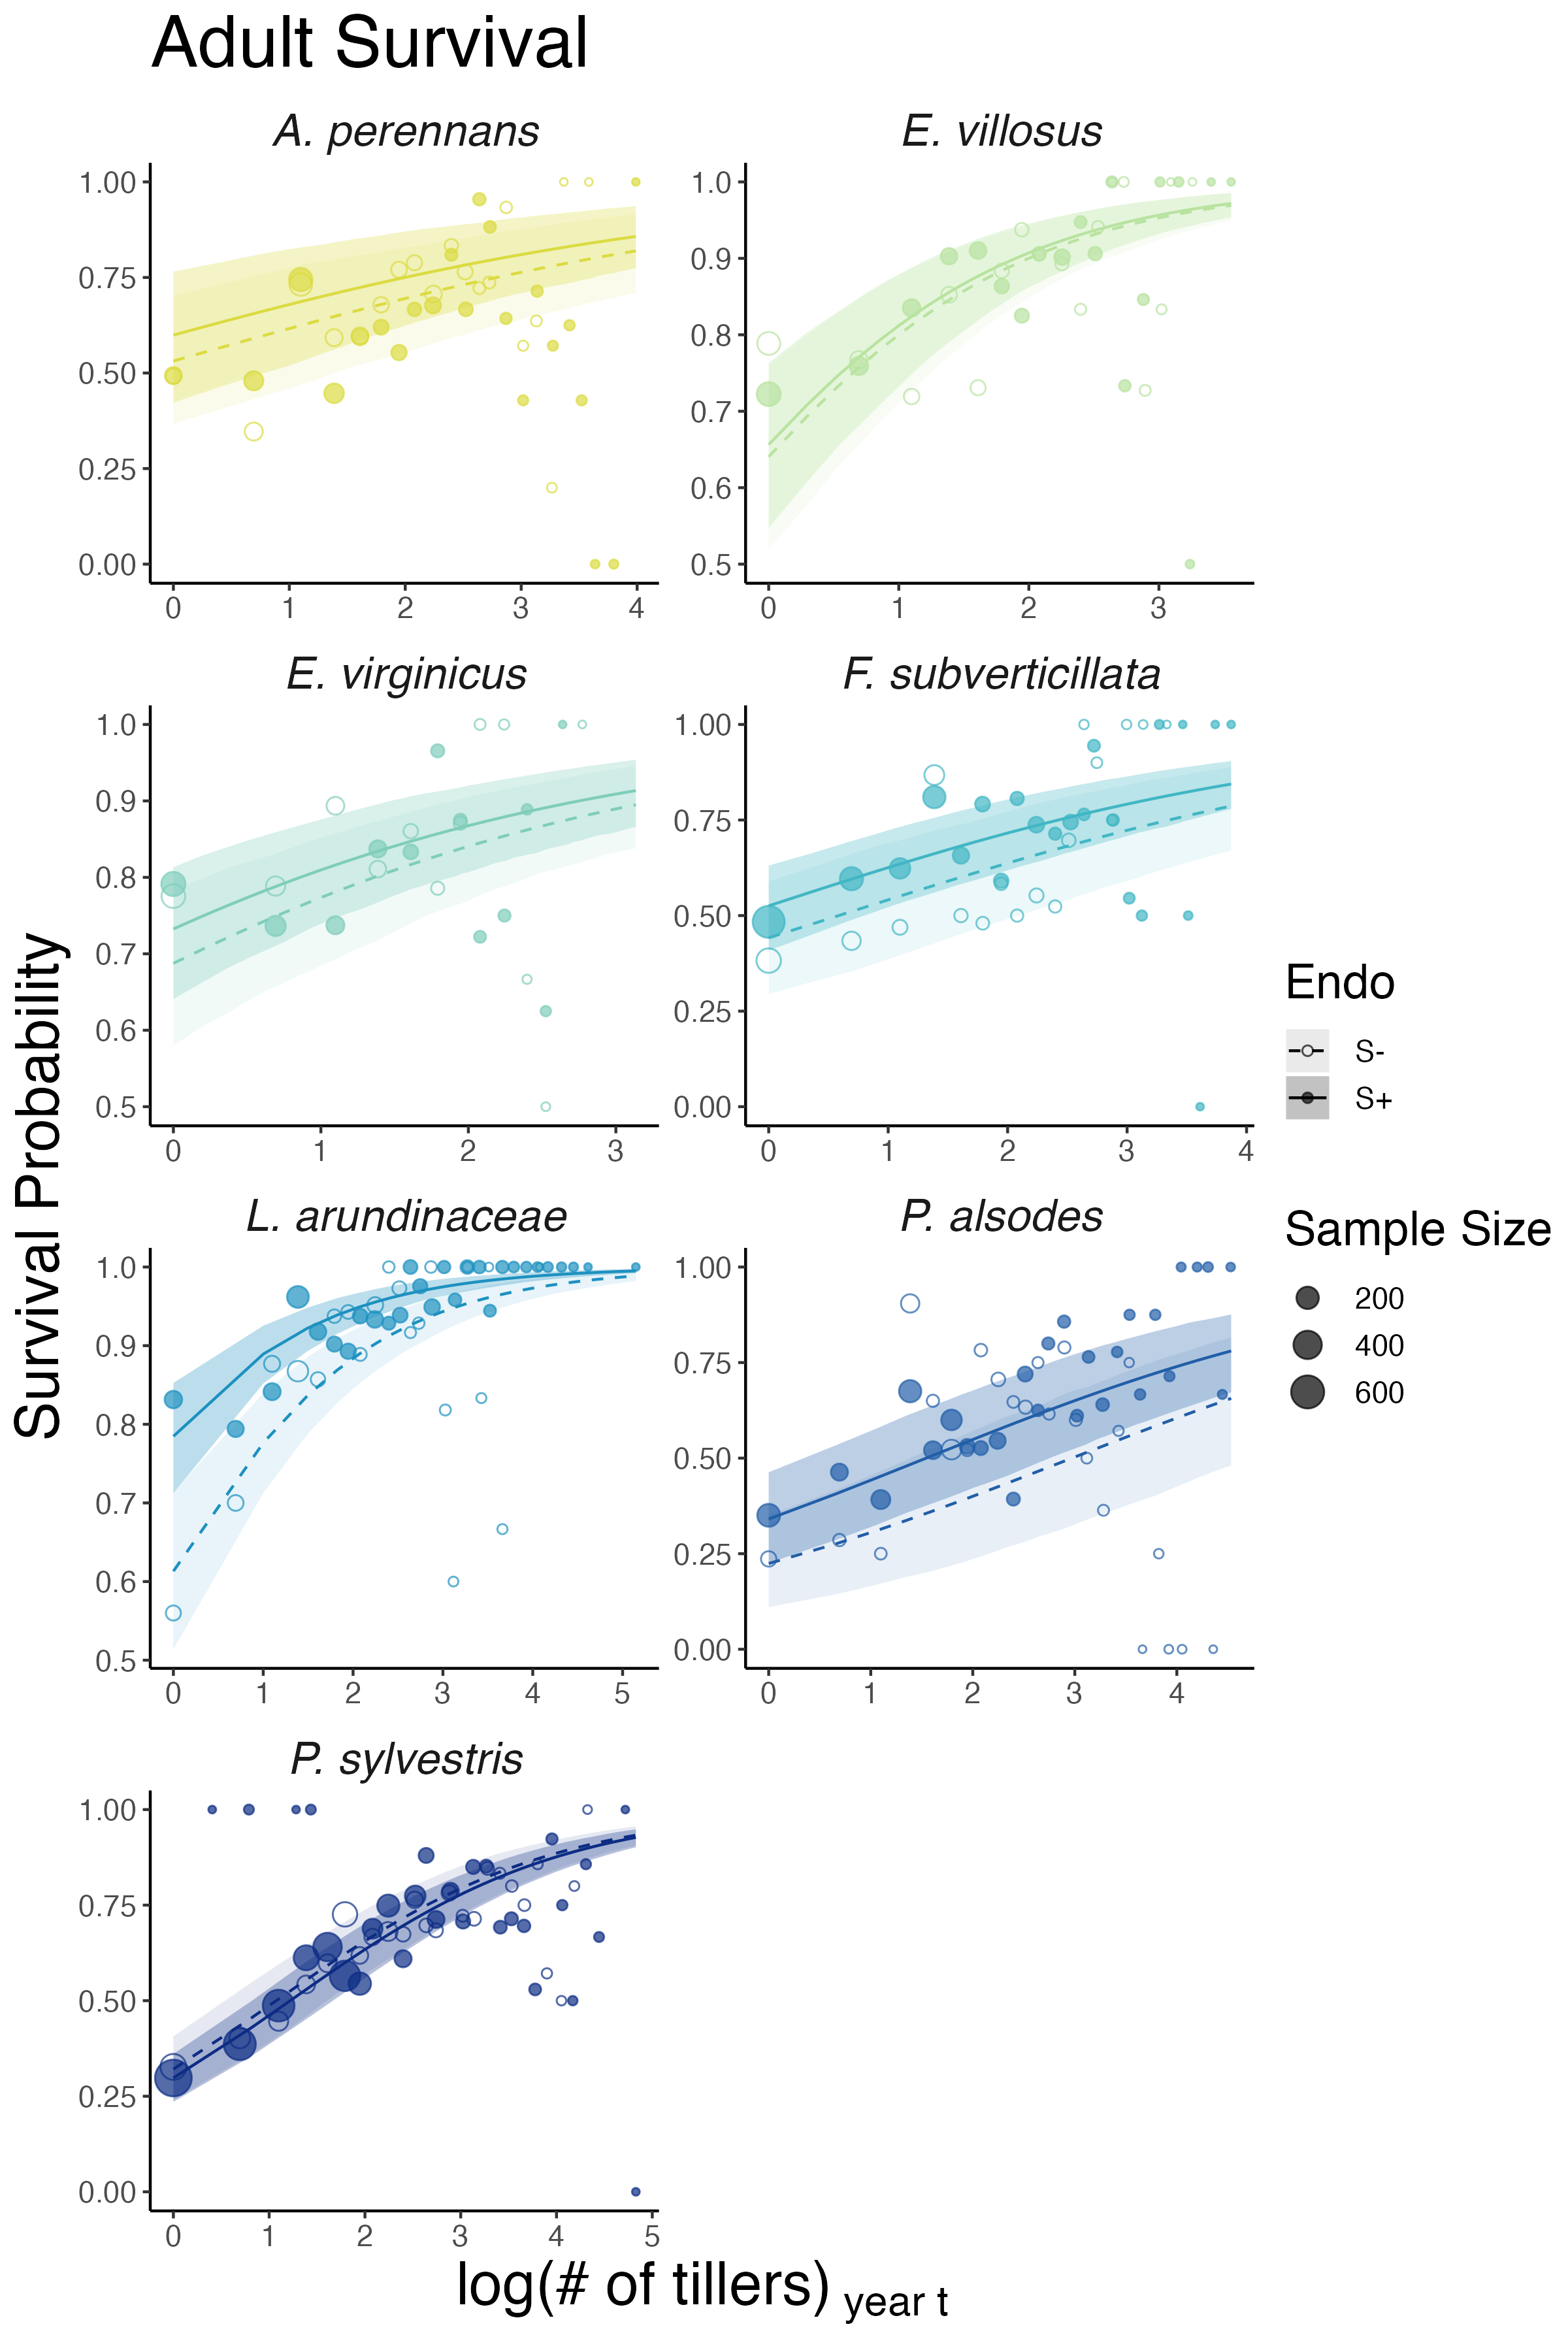
\includegraphics[width=.6\linewidth]{surv_meanplot.png}
	\caption{Effect of endophyte symbiosis on mean adult survival. Fitted curves represent the size-specific mean survival probability along with data binned by size shown as open circles with a dashed line for symbiont-free (S-) plants, while the solid line and filled circles represent symbiontic (S+) plants. 80\% credible intervals are shown with dark shading for  S+, or light shading for S-.}
\end{figure}

\newpage


\begin{figure}
	\centering
	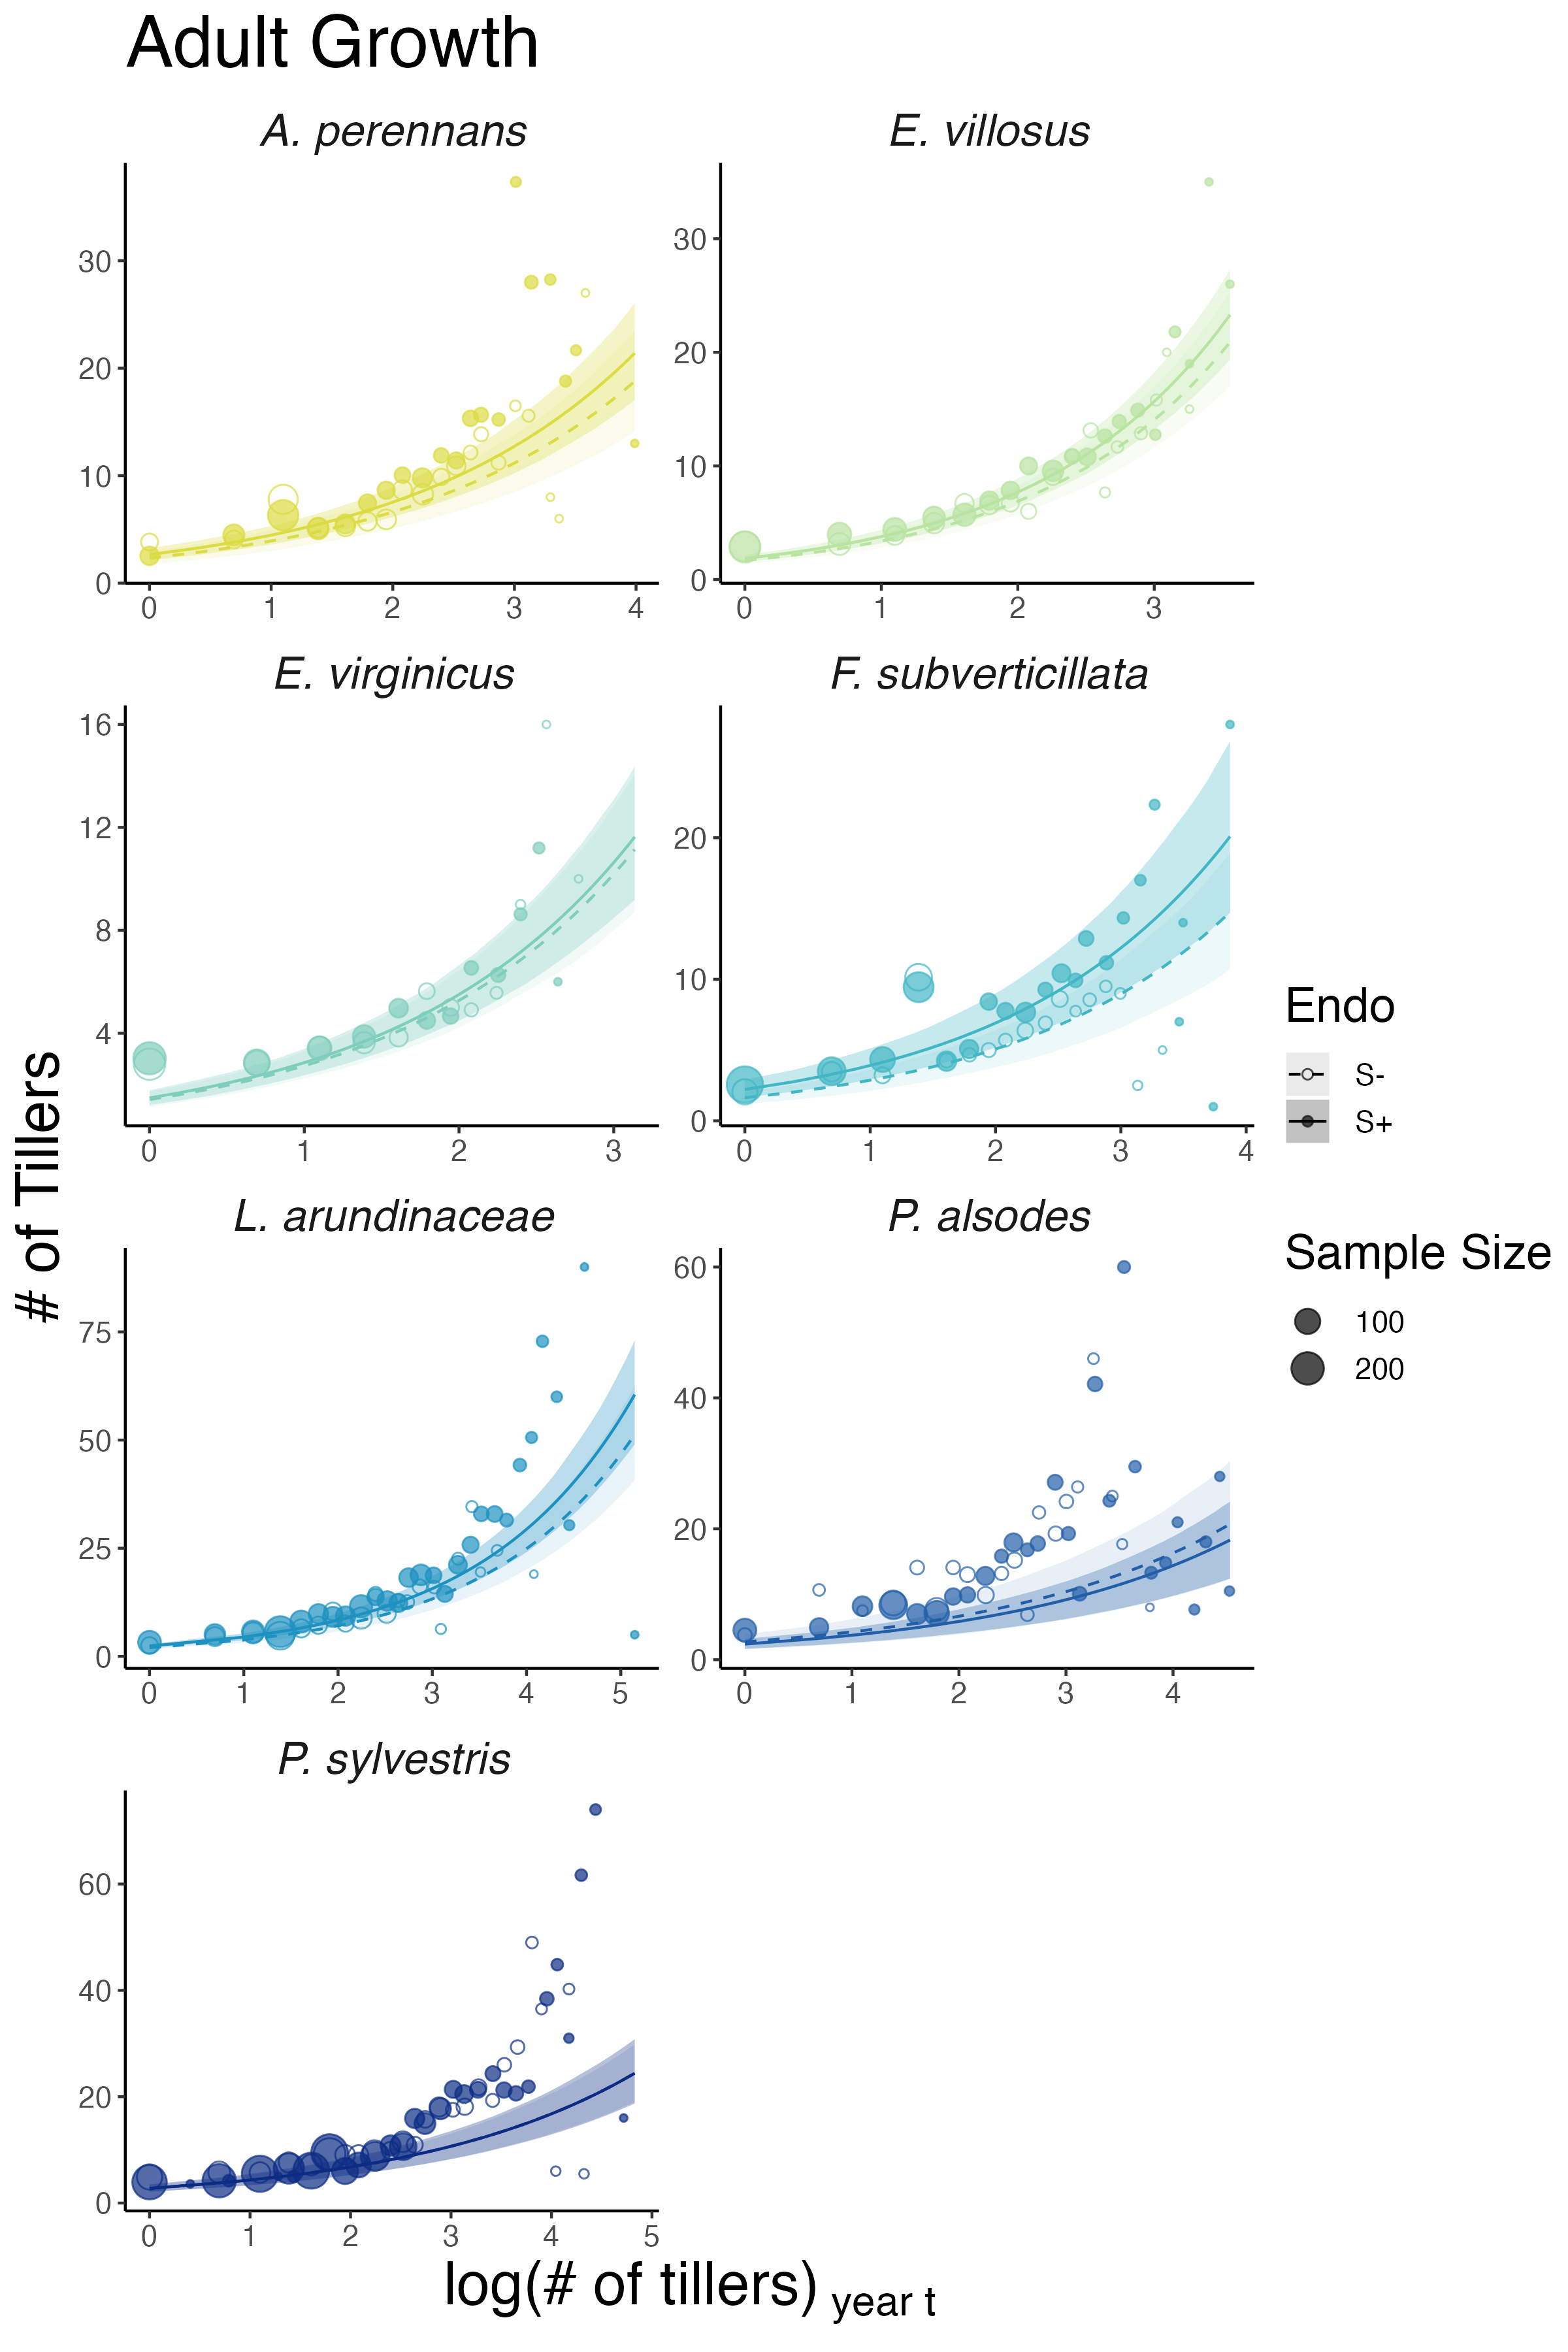
\includegraphics[width=.6\linewidth]{grow_meanplot.png}
	\caption{Effect of endophyte symbiosis on mean adult growth. Fitted curves represent the size-specific mean expected plant size along with data binned by size shown as open circles with a dashed line for symbiont-free (S-) plants, while the solid line and filled circles represent symbiontic (S+) plants. 80\% credible intervals are shown with dark shading for  S+, or light shading for S-.}
\end{figure}


\begin{figure}
	\centering
	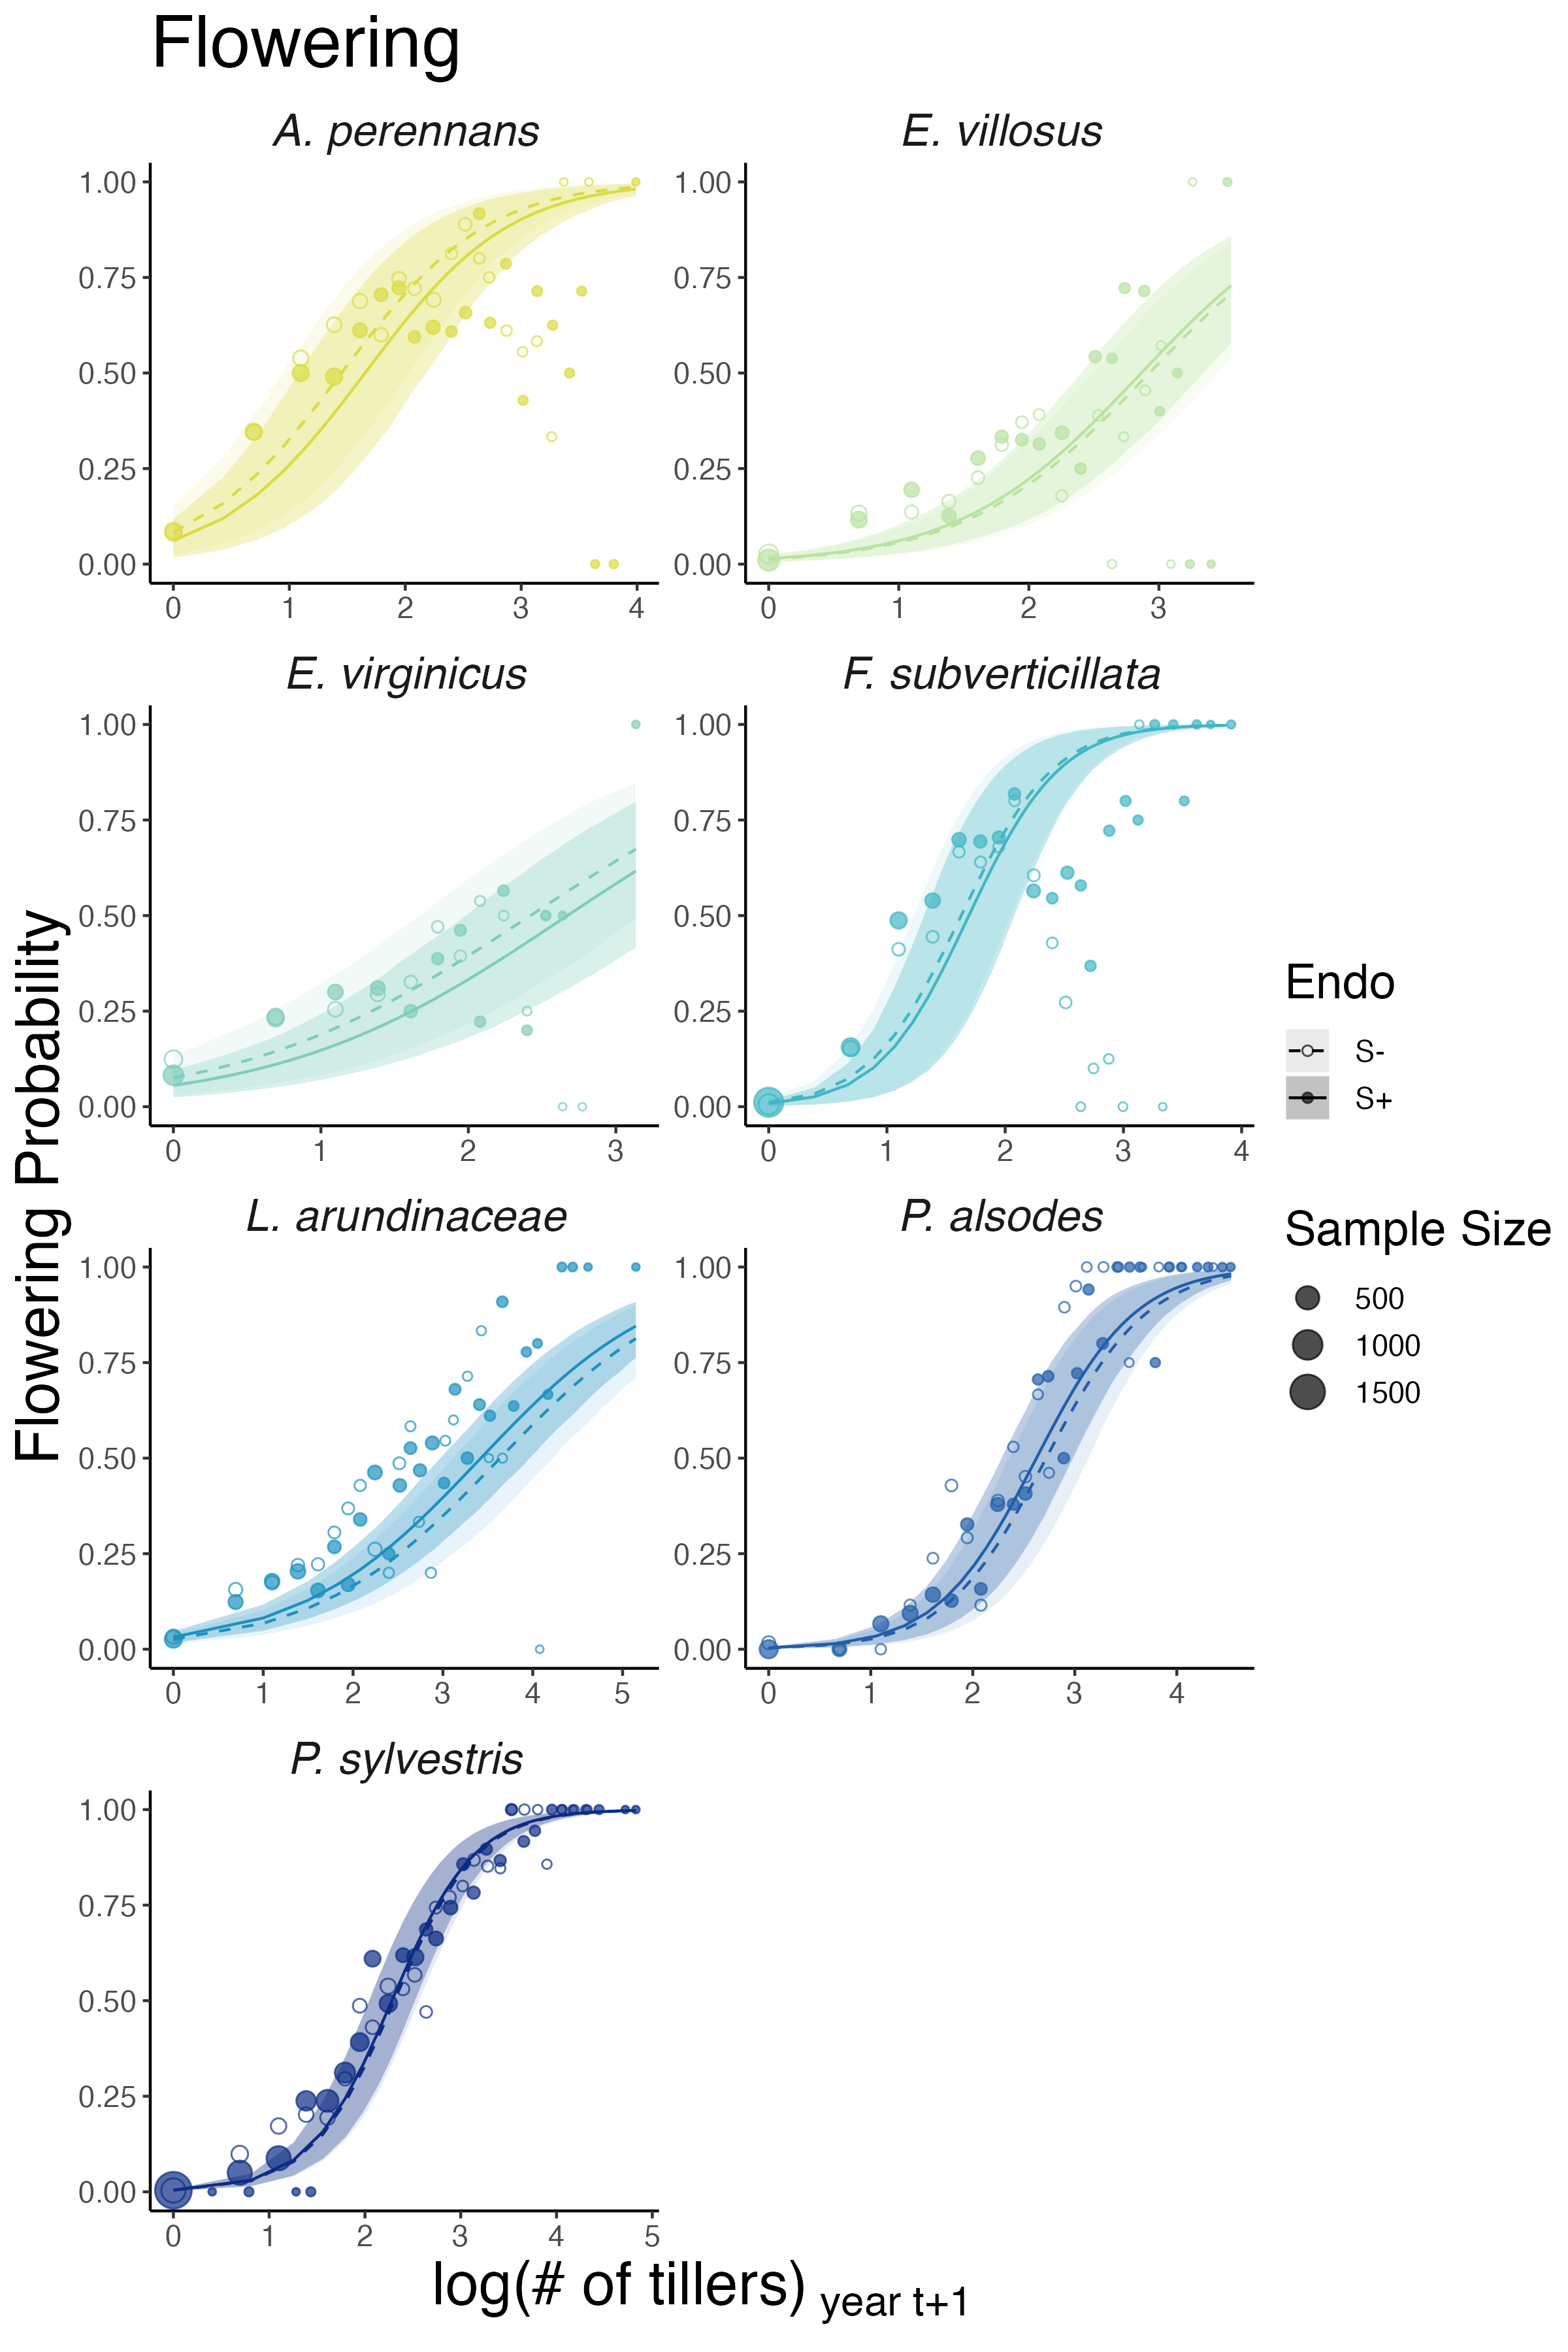
\includegraphics[width=.6\linewidth]{flw_meanplot.png}
	\caption{Effect of endophyte symbiosis on mean flowering. Fitted curves represent the size-specific mean flowering probability along with data binned by size shown as open circles with a dashed line for symbiont-free (S-) plants, while the solid line and filled circles represent symbiontic (S+) plants. 80\% credible intervals are shown with dark shading for  S+, or light shading for S-.}
\end{figure}


\begin{figure}
	\centering
	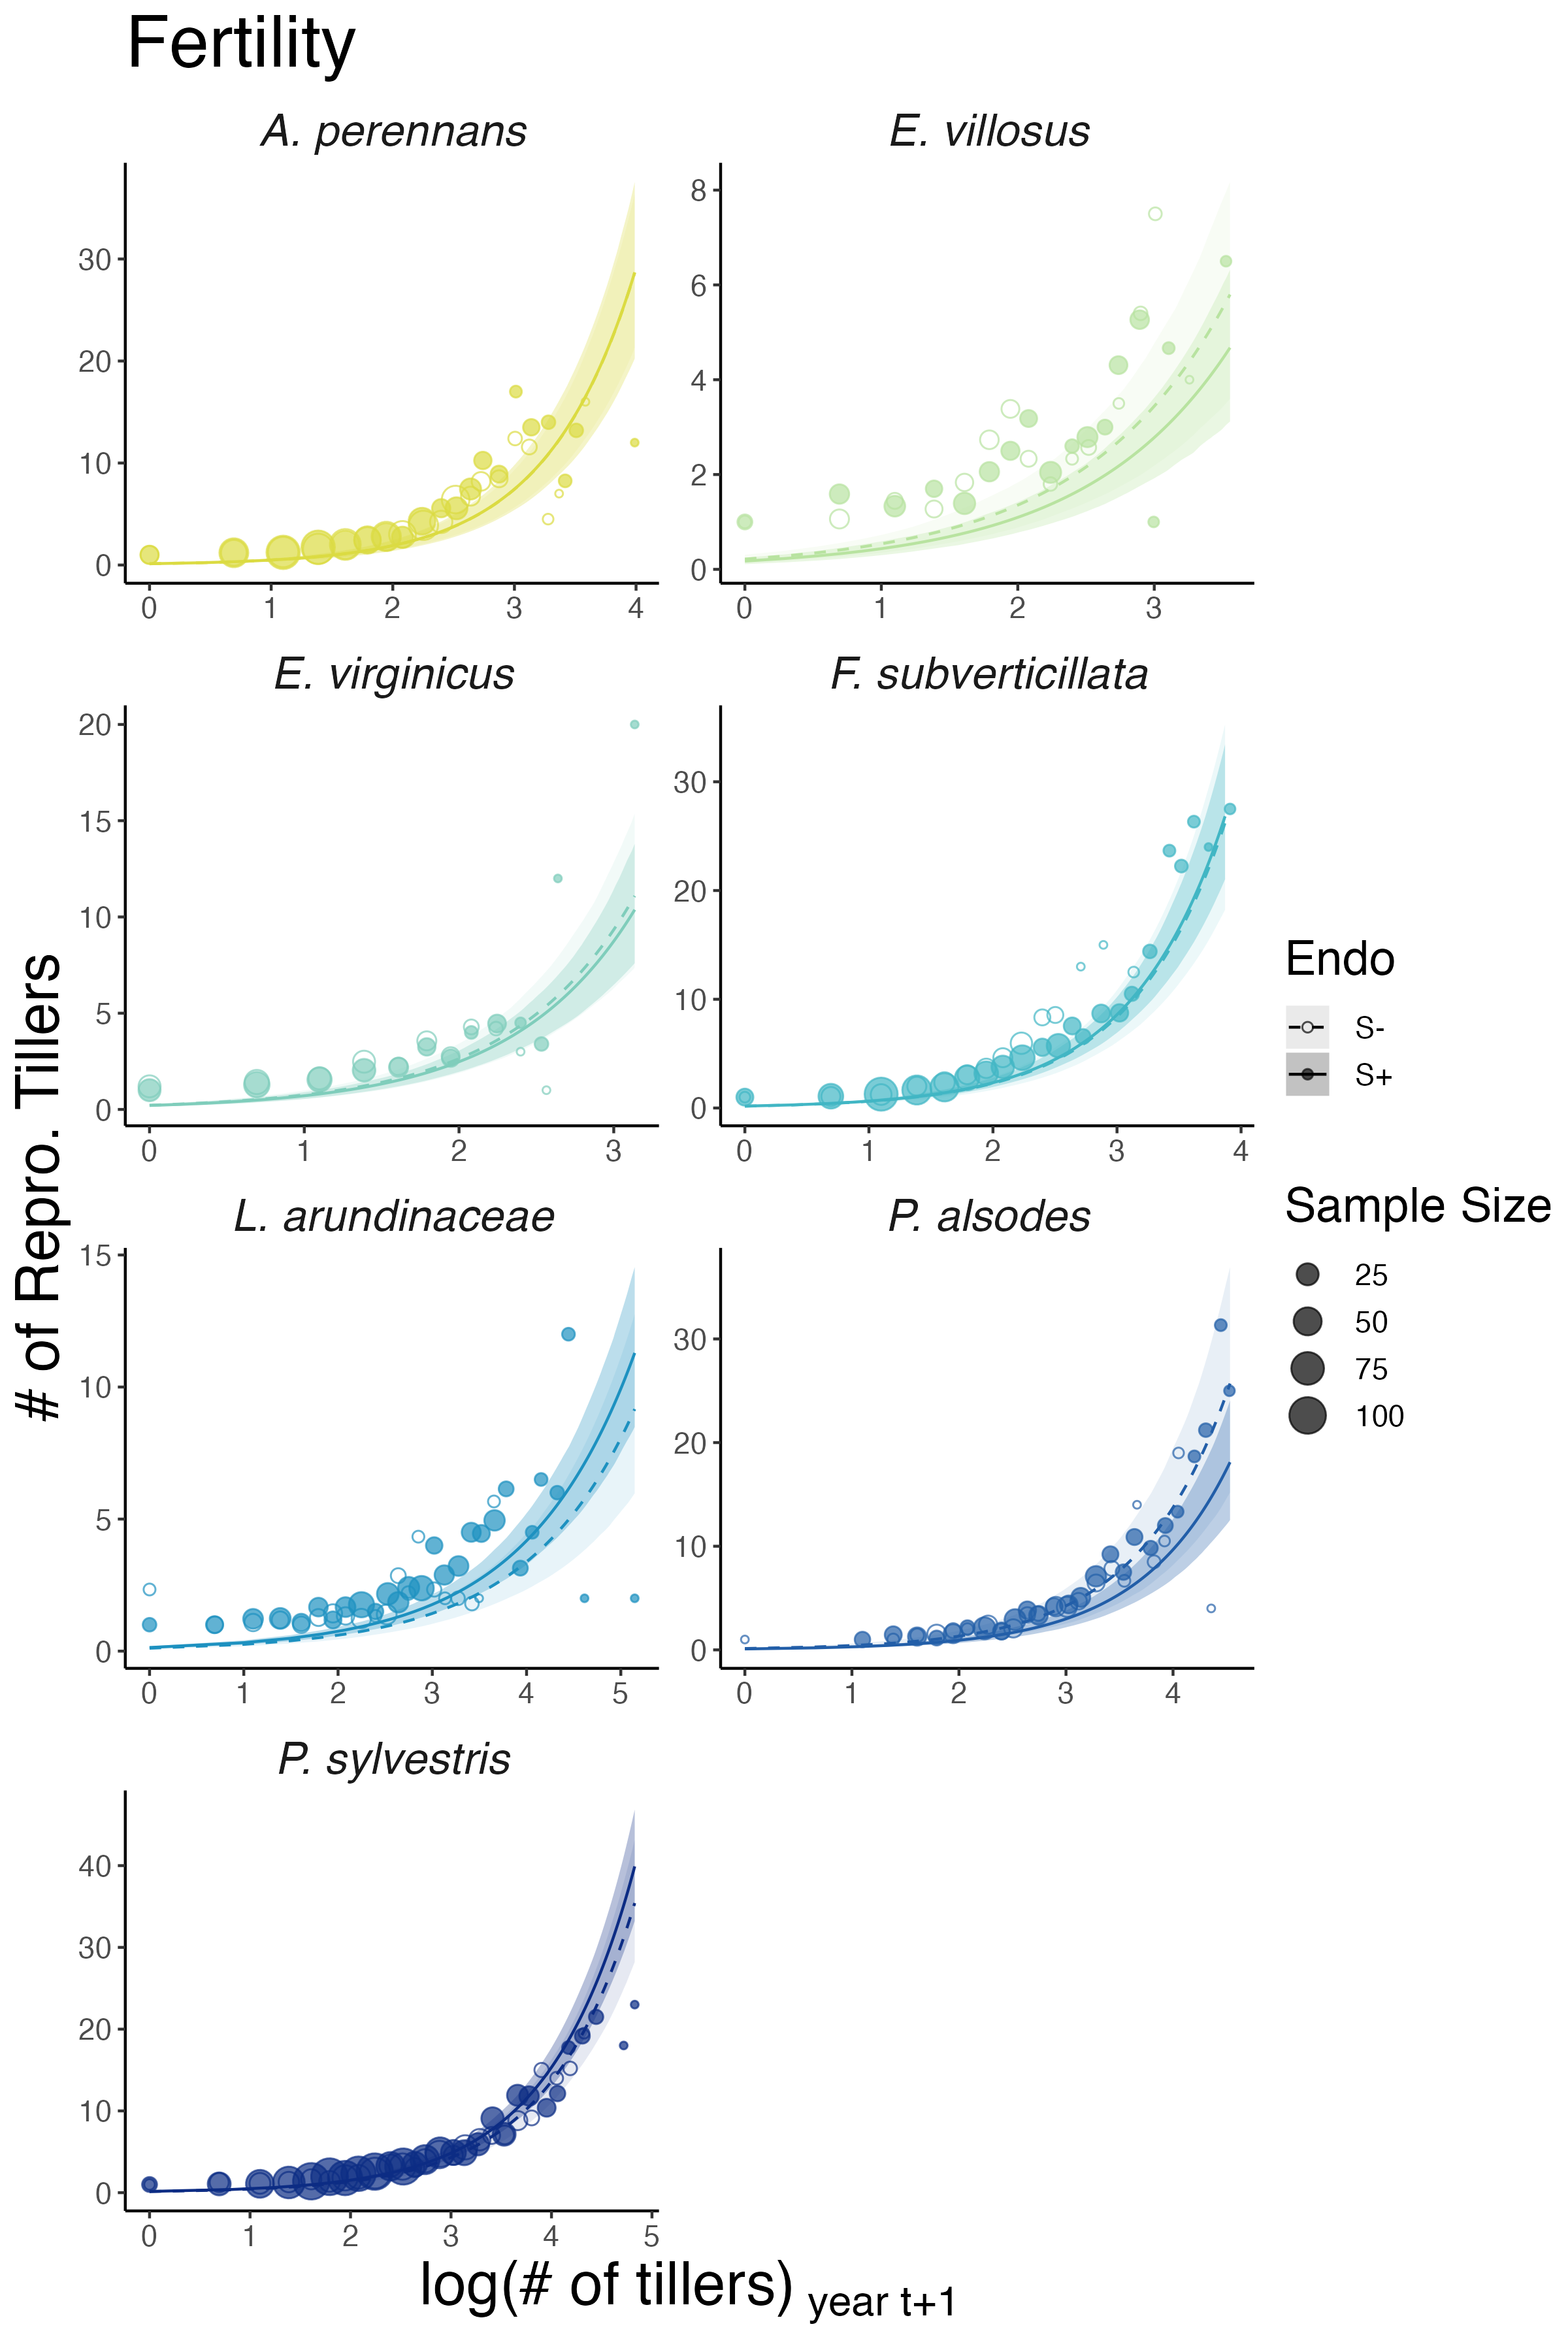
\includegraphics[width=.6\linewidth]{fert_meanplot.png}
	\caption{Effect of endophyte symbiosis on mean fertility. Fitted curves represent the size-specific mean expected number of flowering tillers along with data binned by size shown as open circles with a dashed line for symbiont-free (S-) plants, while the solid line and filled circles represent symbiontic (S+) plants. 80\% credible intervals are shown with dark shading for  S+, or light shading for S-.}
\end{figure}


\begin{figure}
	\centering
	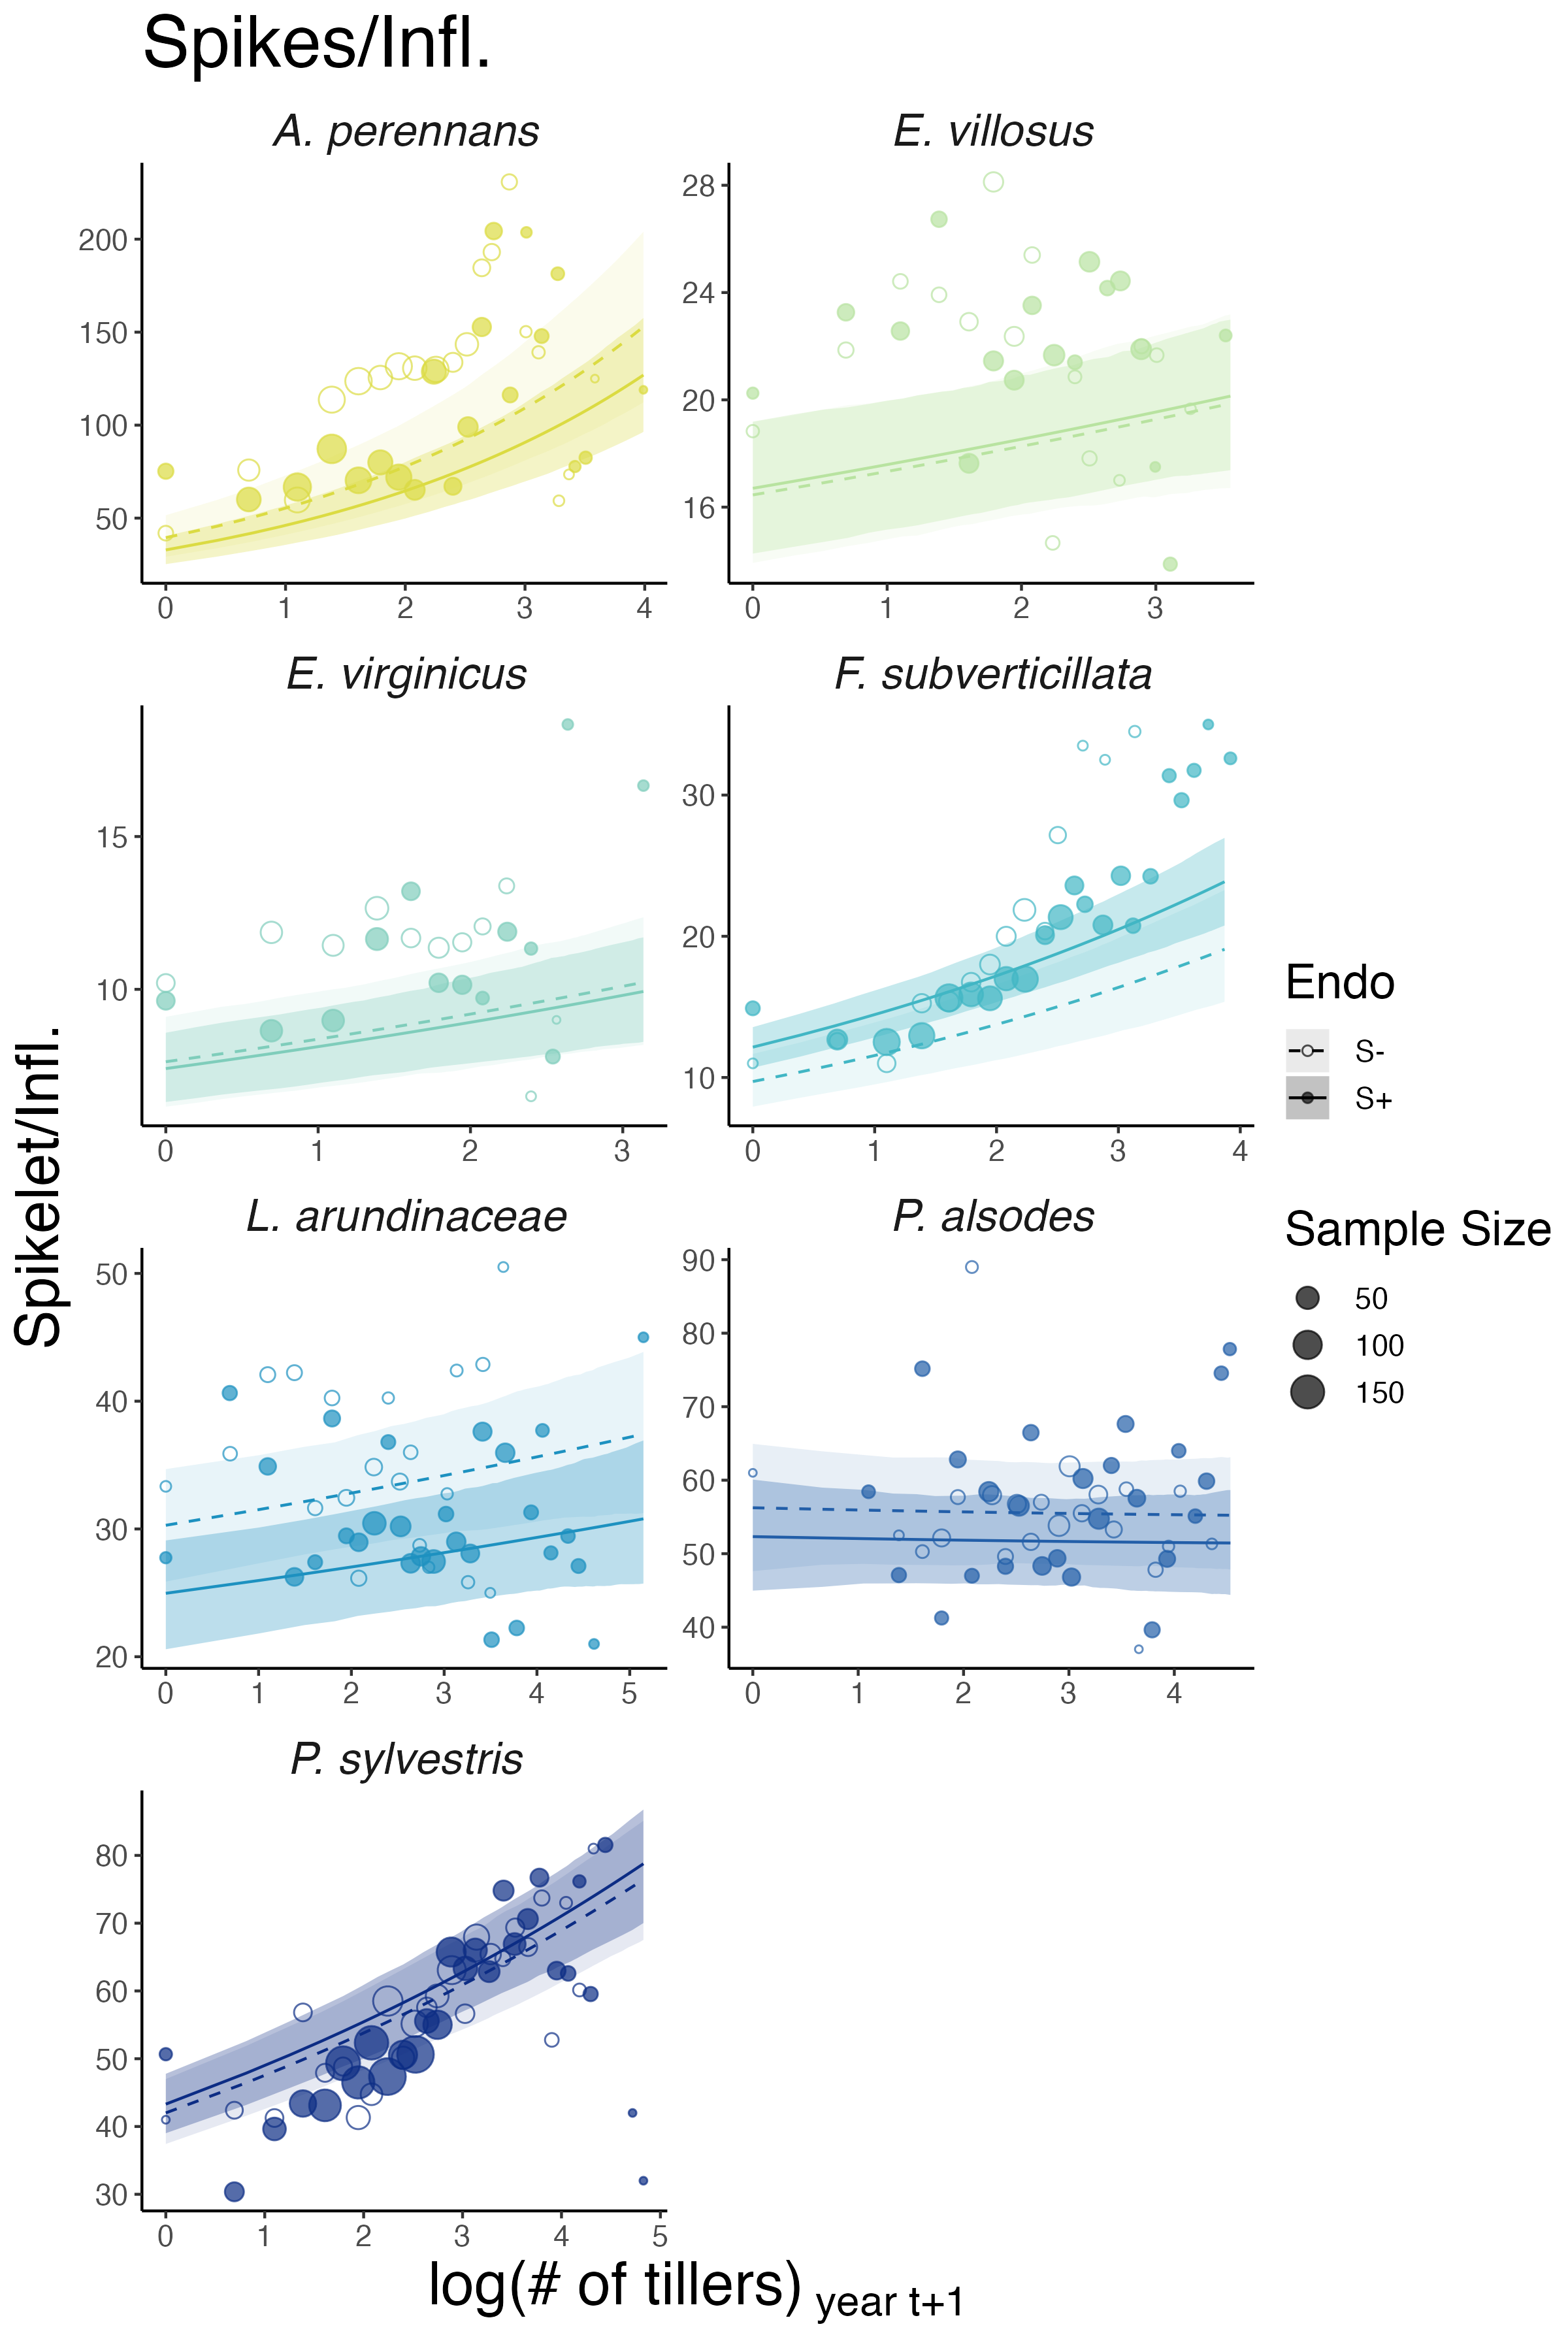
\includegraphics[width=.6\linewidth]{spike_meanplot.png}
	\caption{Effect of endophyte symbiosis on mean spikelet production. Fitted curves represent the size-specific mean expected number of spikelets per inflorescence along with data binned by size shown as open circles with a dashed line for symbiont-free (S-) plants, while the solid line and filled circles represent symbiontic (S+) plants. 80\% credible intervals are shown with dark shading for  S+, or light shading for S-.}
\end{figure}


\begin{figure}
	\centering
	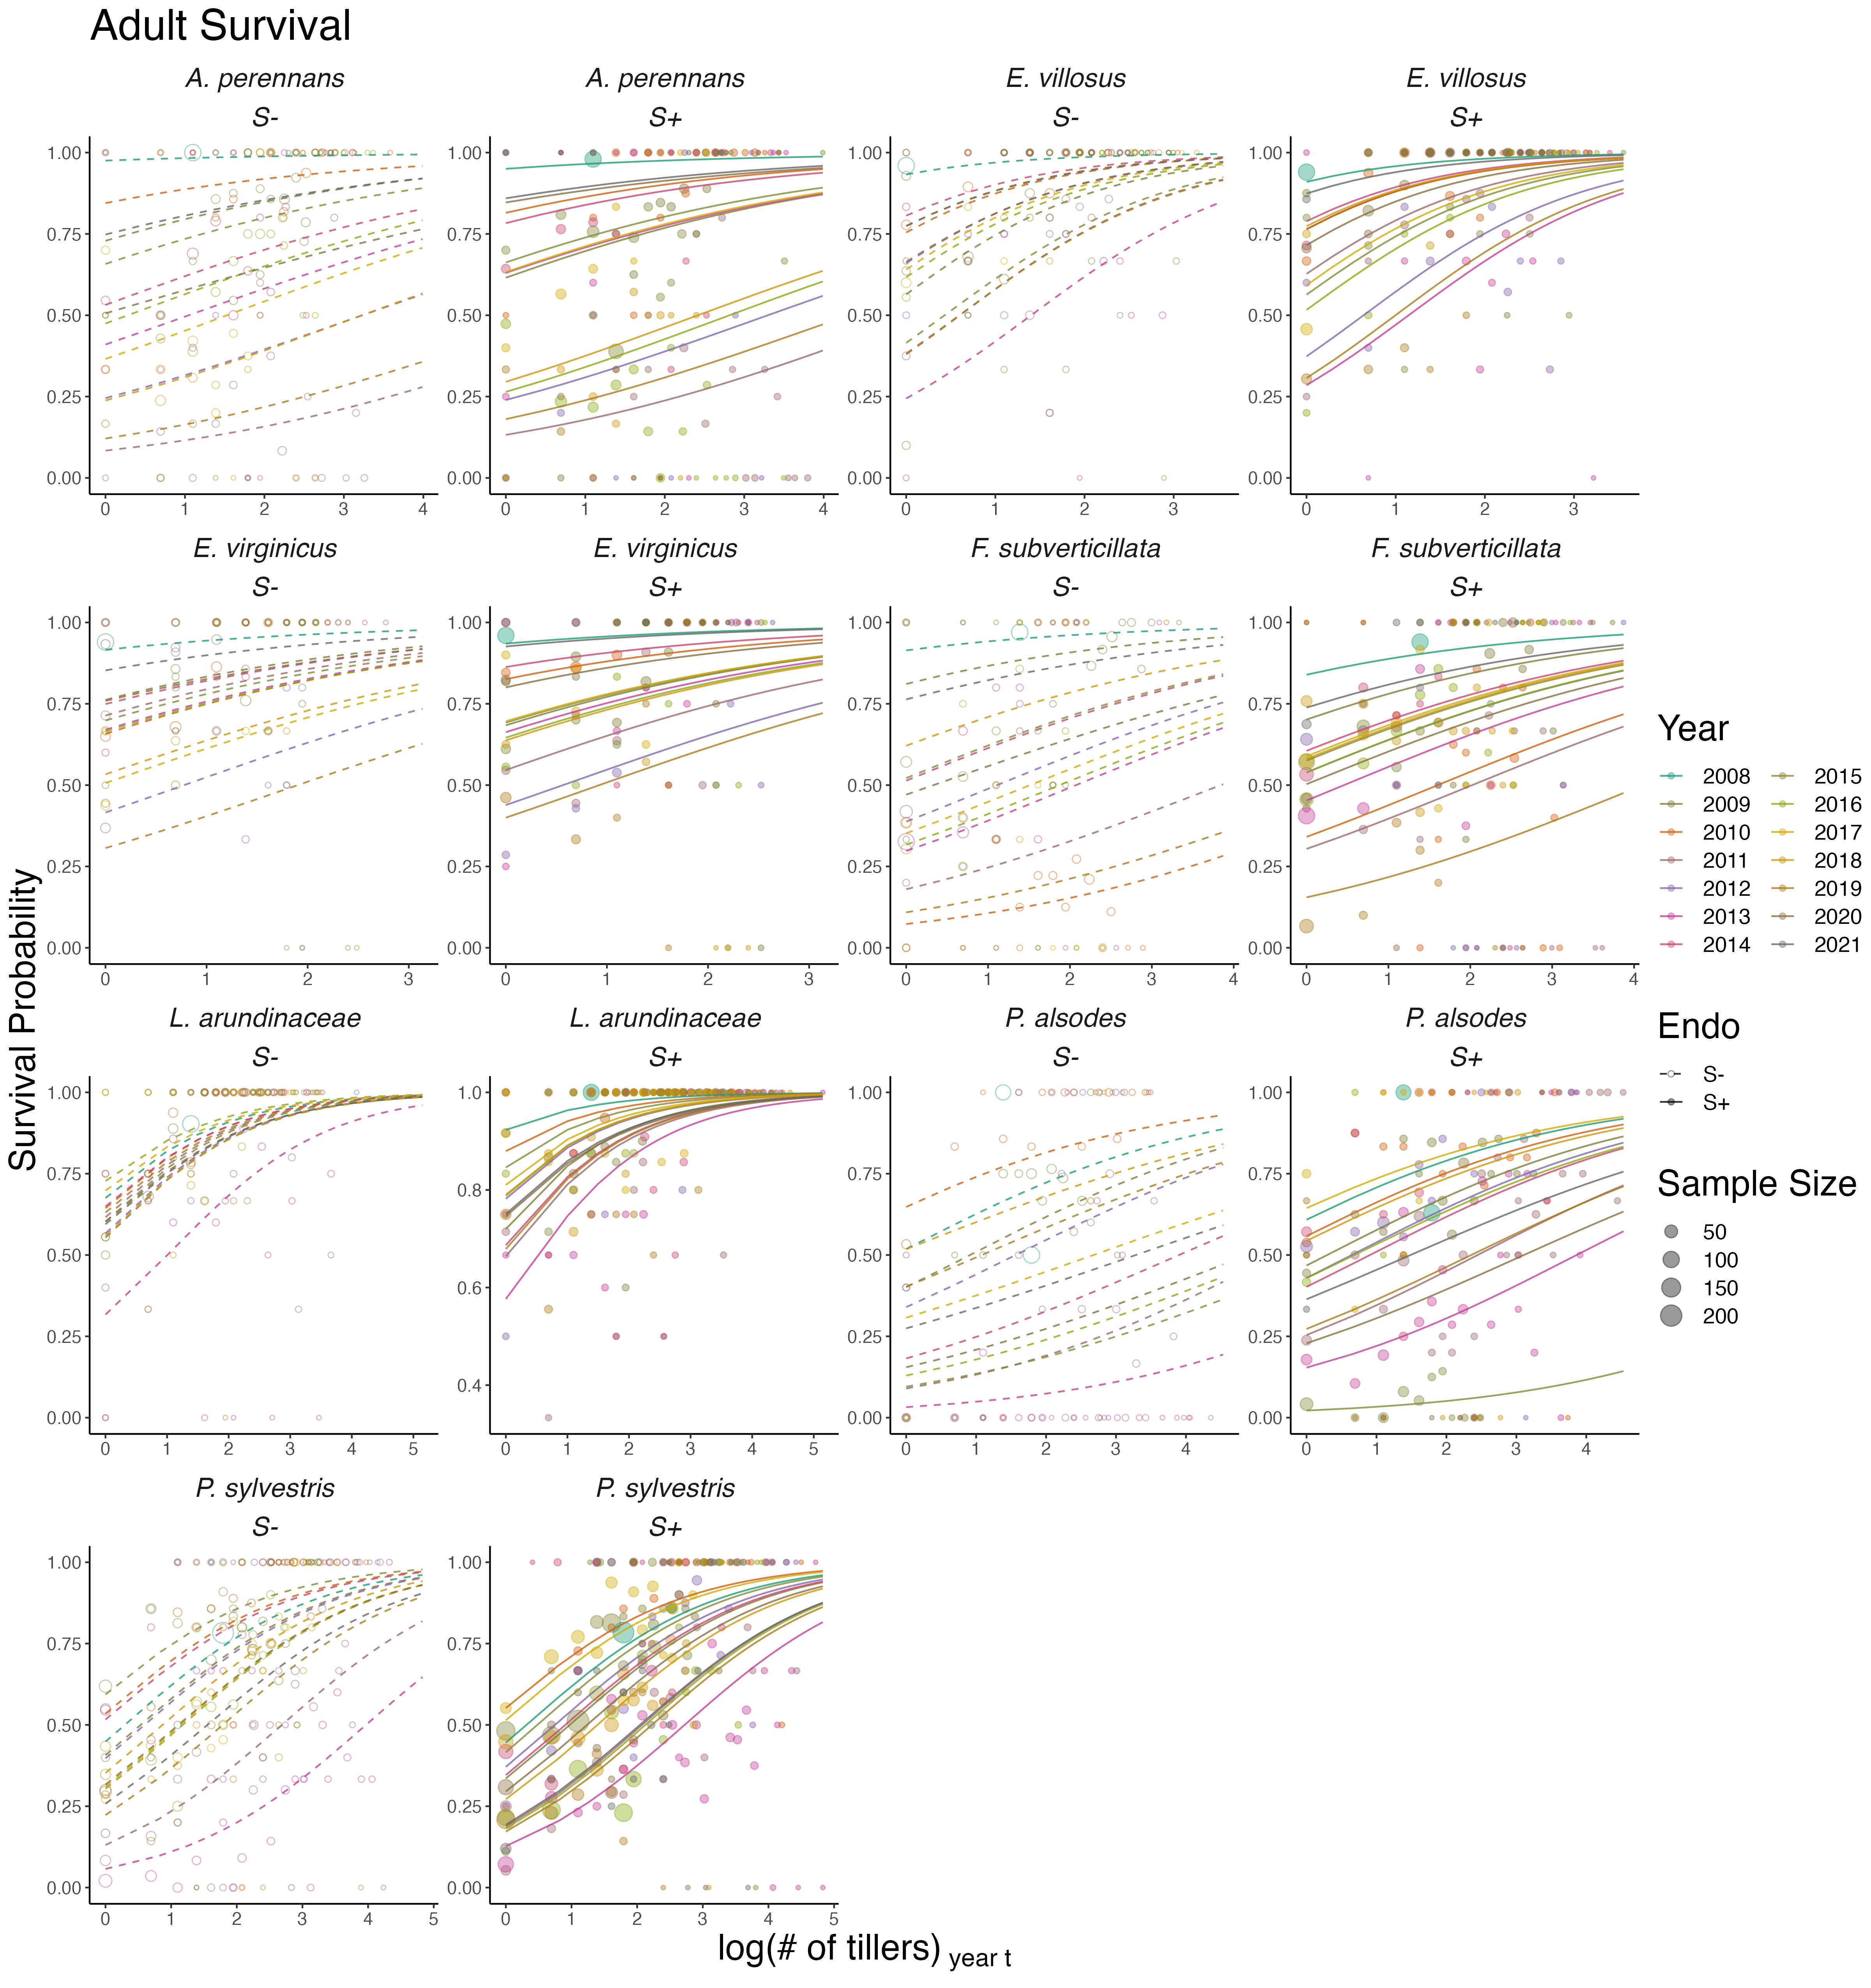
\includegraphics[width=\linewidth]{surv_yearplot.png}
	\caption{Effect of endophyte symbiosis on yearly adult survival. Fitted curves represent the size-specific annual survival probability along with data binned by size and census year shown as open circles with a dashed line for symbiont-free (S-) plants, while the solid line and filled circles represent symbiontic (S+) plants. }
\end{figure}


\begin{figure}
	\centering
	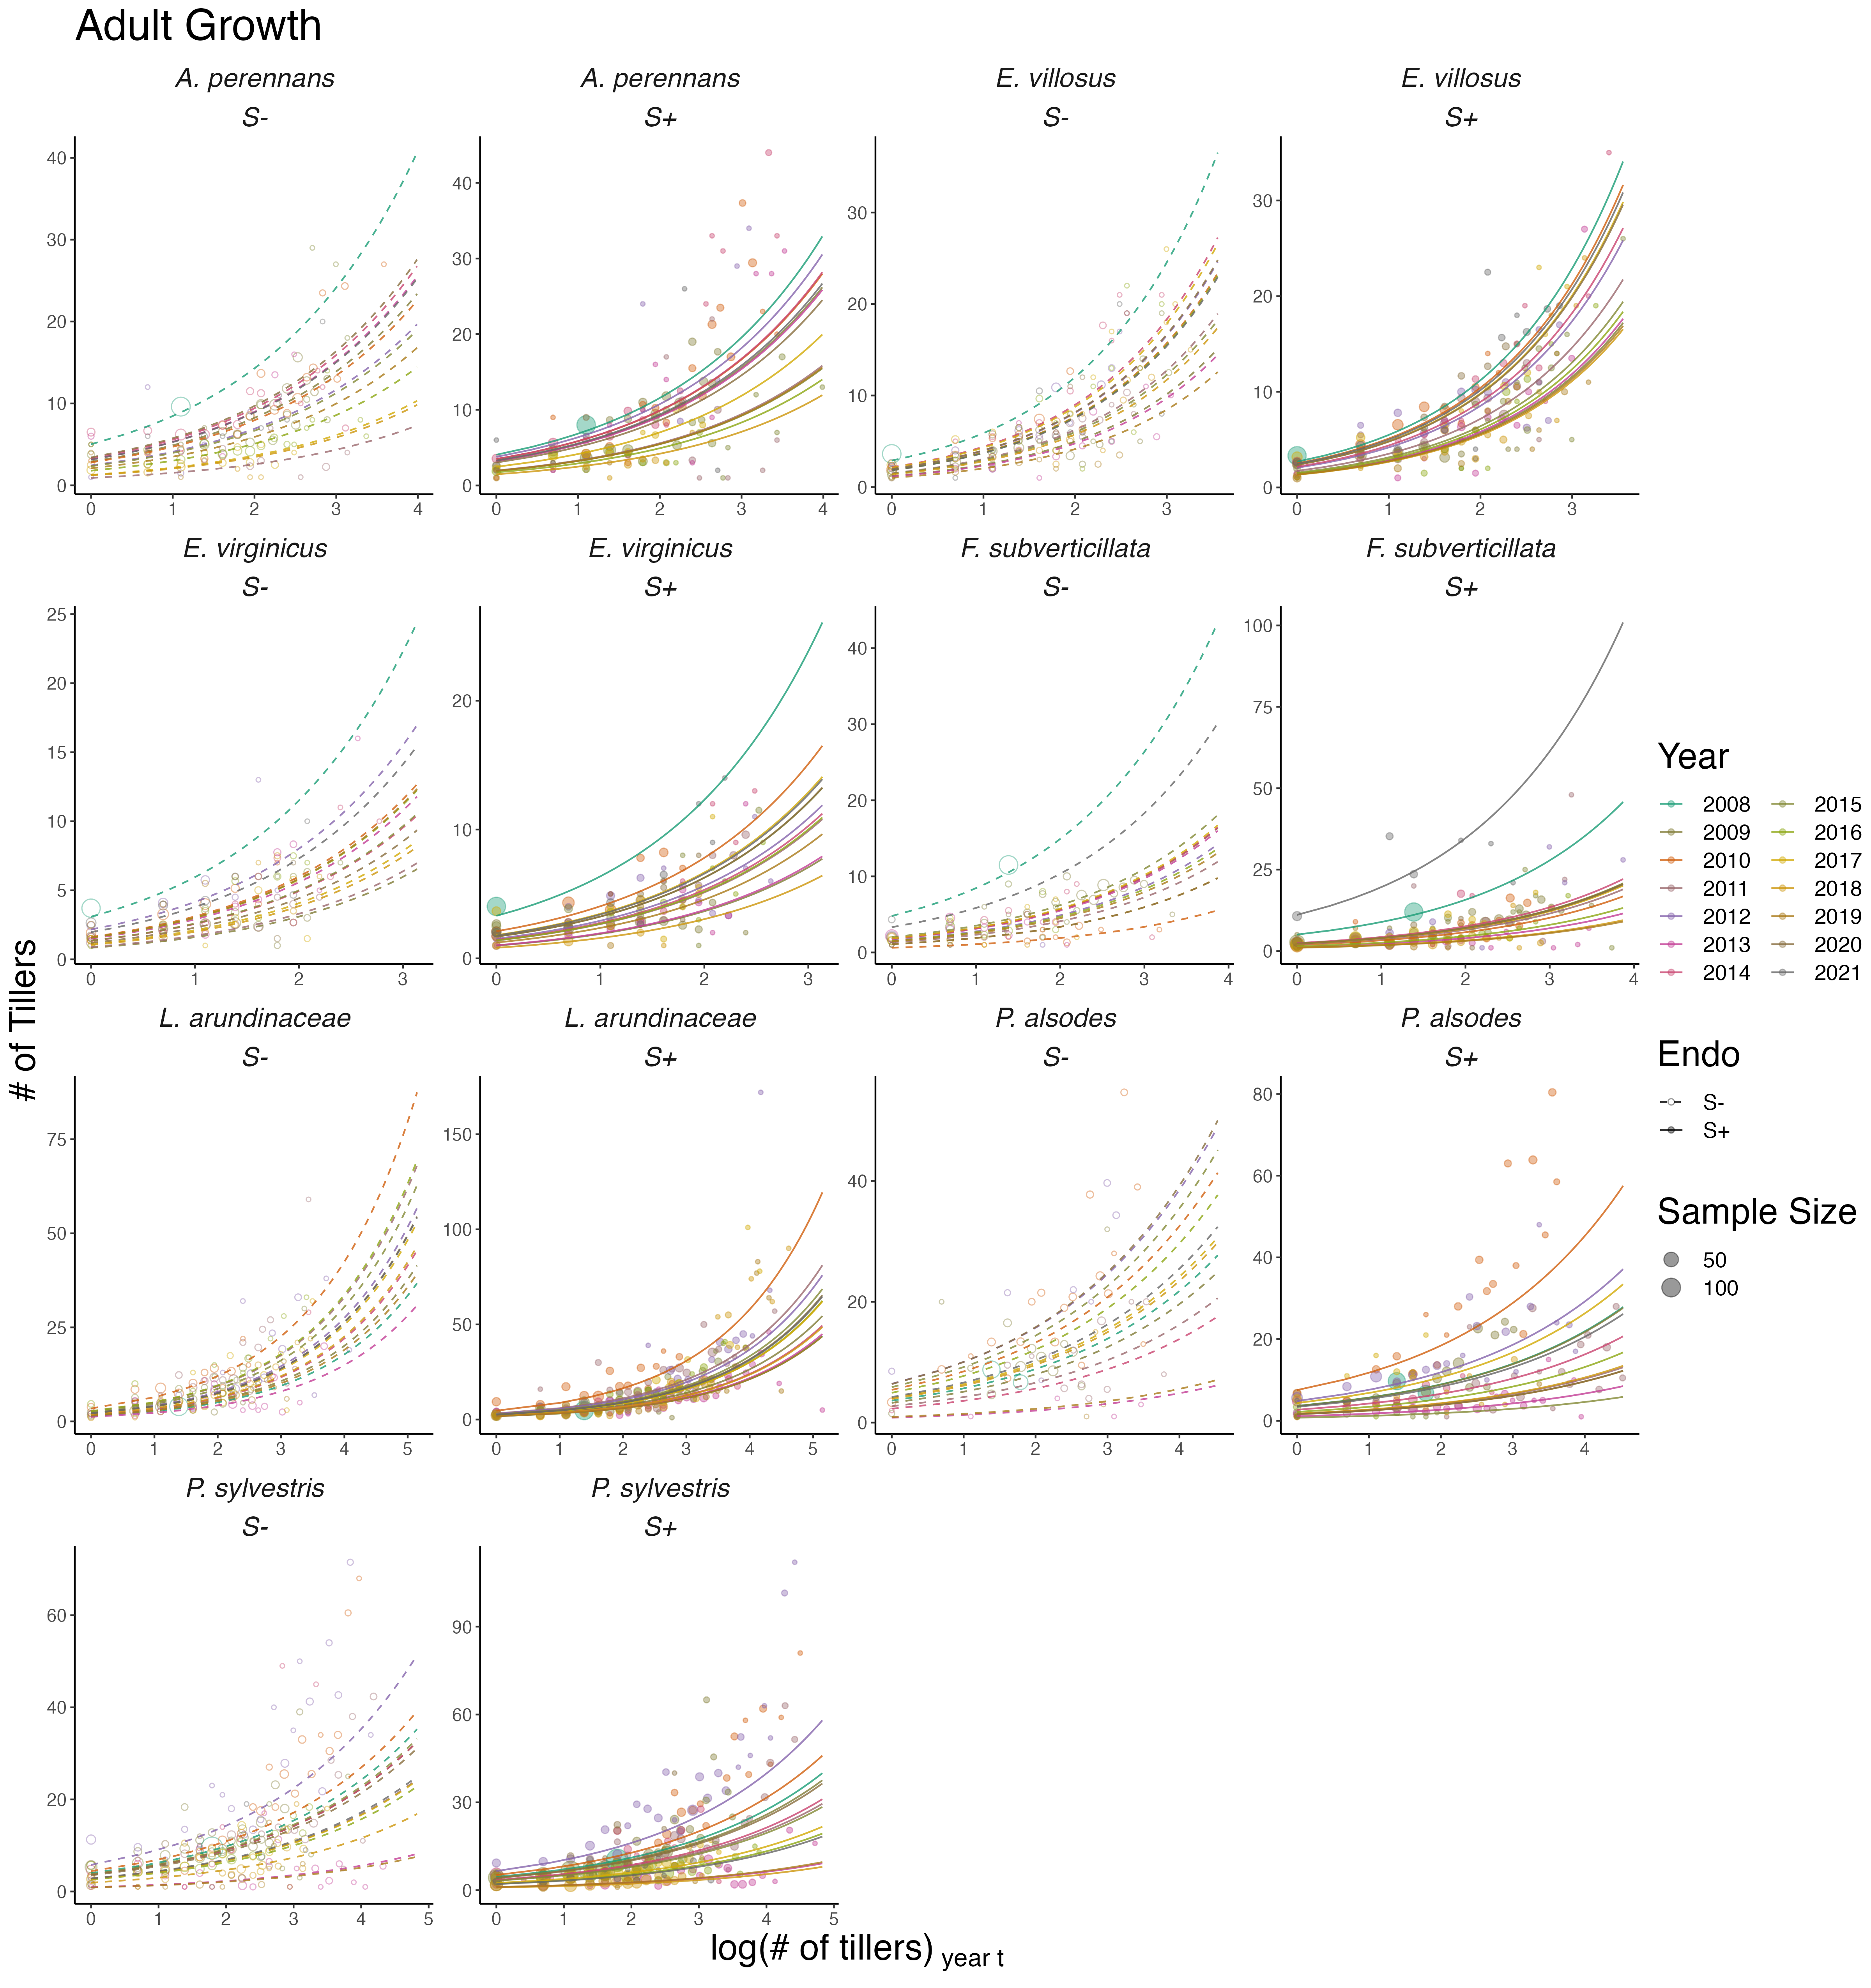
\includegraphics[width=\linewidth]{grow_yearplot.png}
	\caption{Effect of endophyte symbiosis on yearly adult growth. Fitted curves represent the size-specific annual expected plant size along with data binned by size and census year shown as open circles with a dashed line for symbiont-free (S-) plants, while the solid line and filled circles represent symbiontic (S+) plants. }
\end{figure}


\begin{figure}
	\centering
	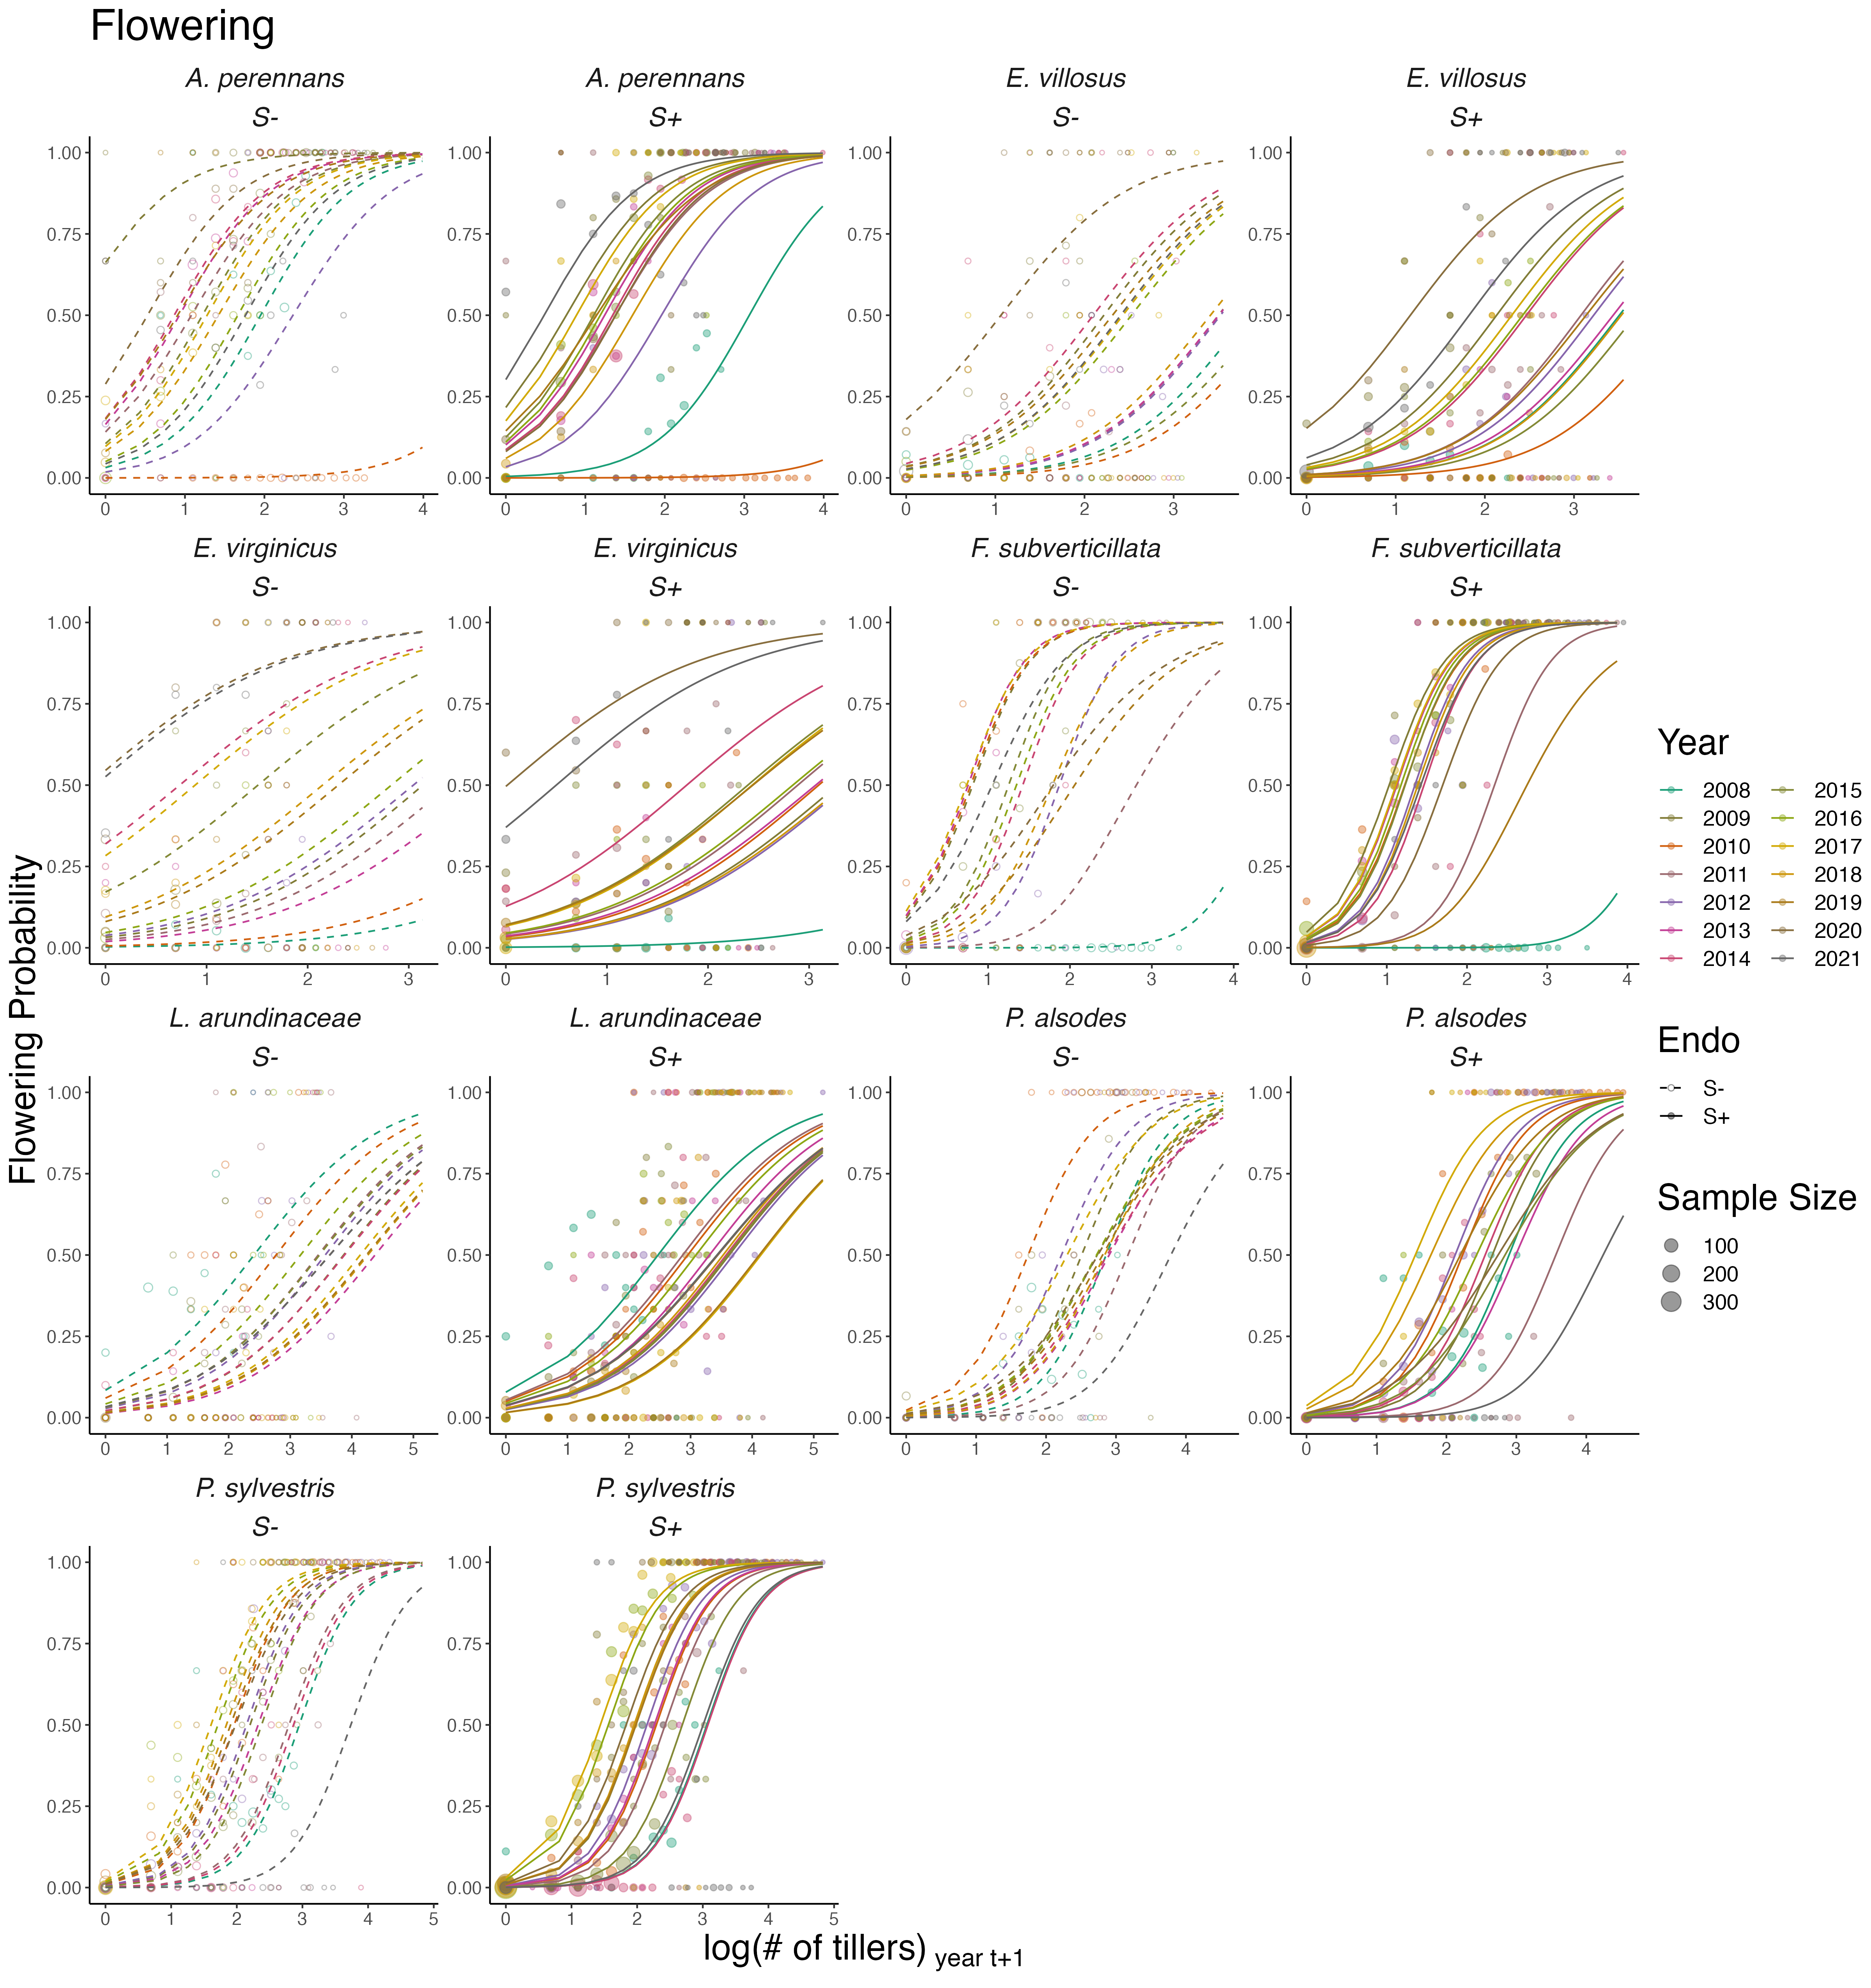
\includegraphics[width=\linewidth]{flw_yearplot.png}
	\caption{Effect of endophyte symbiosis on yearly flowering. Fitted curves represent the size-specific annual flowering probability along with data binned by size and census year shown as open circles with a dashed line for symbiont-free (S-) plants, while the solid line and filled circles represent symbiontic (S+) plants.}
\end{figure}


\begin{figure}
	\centering
	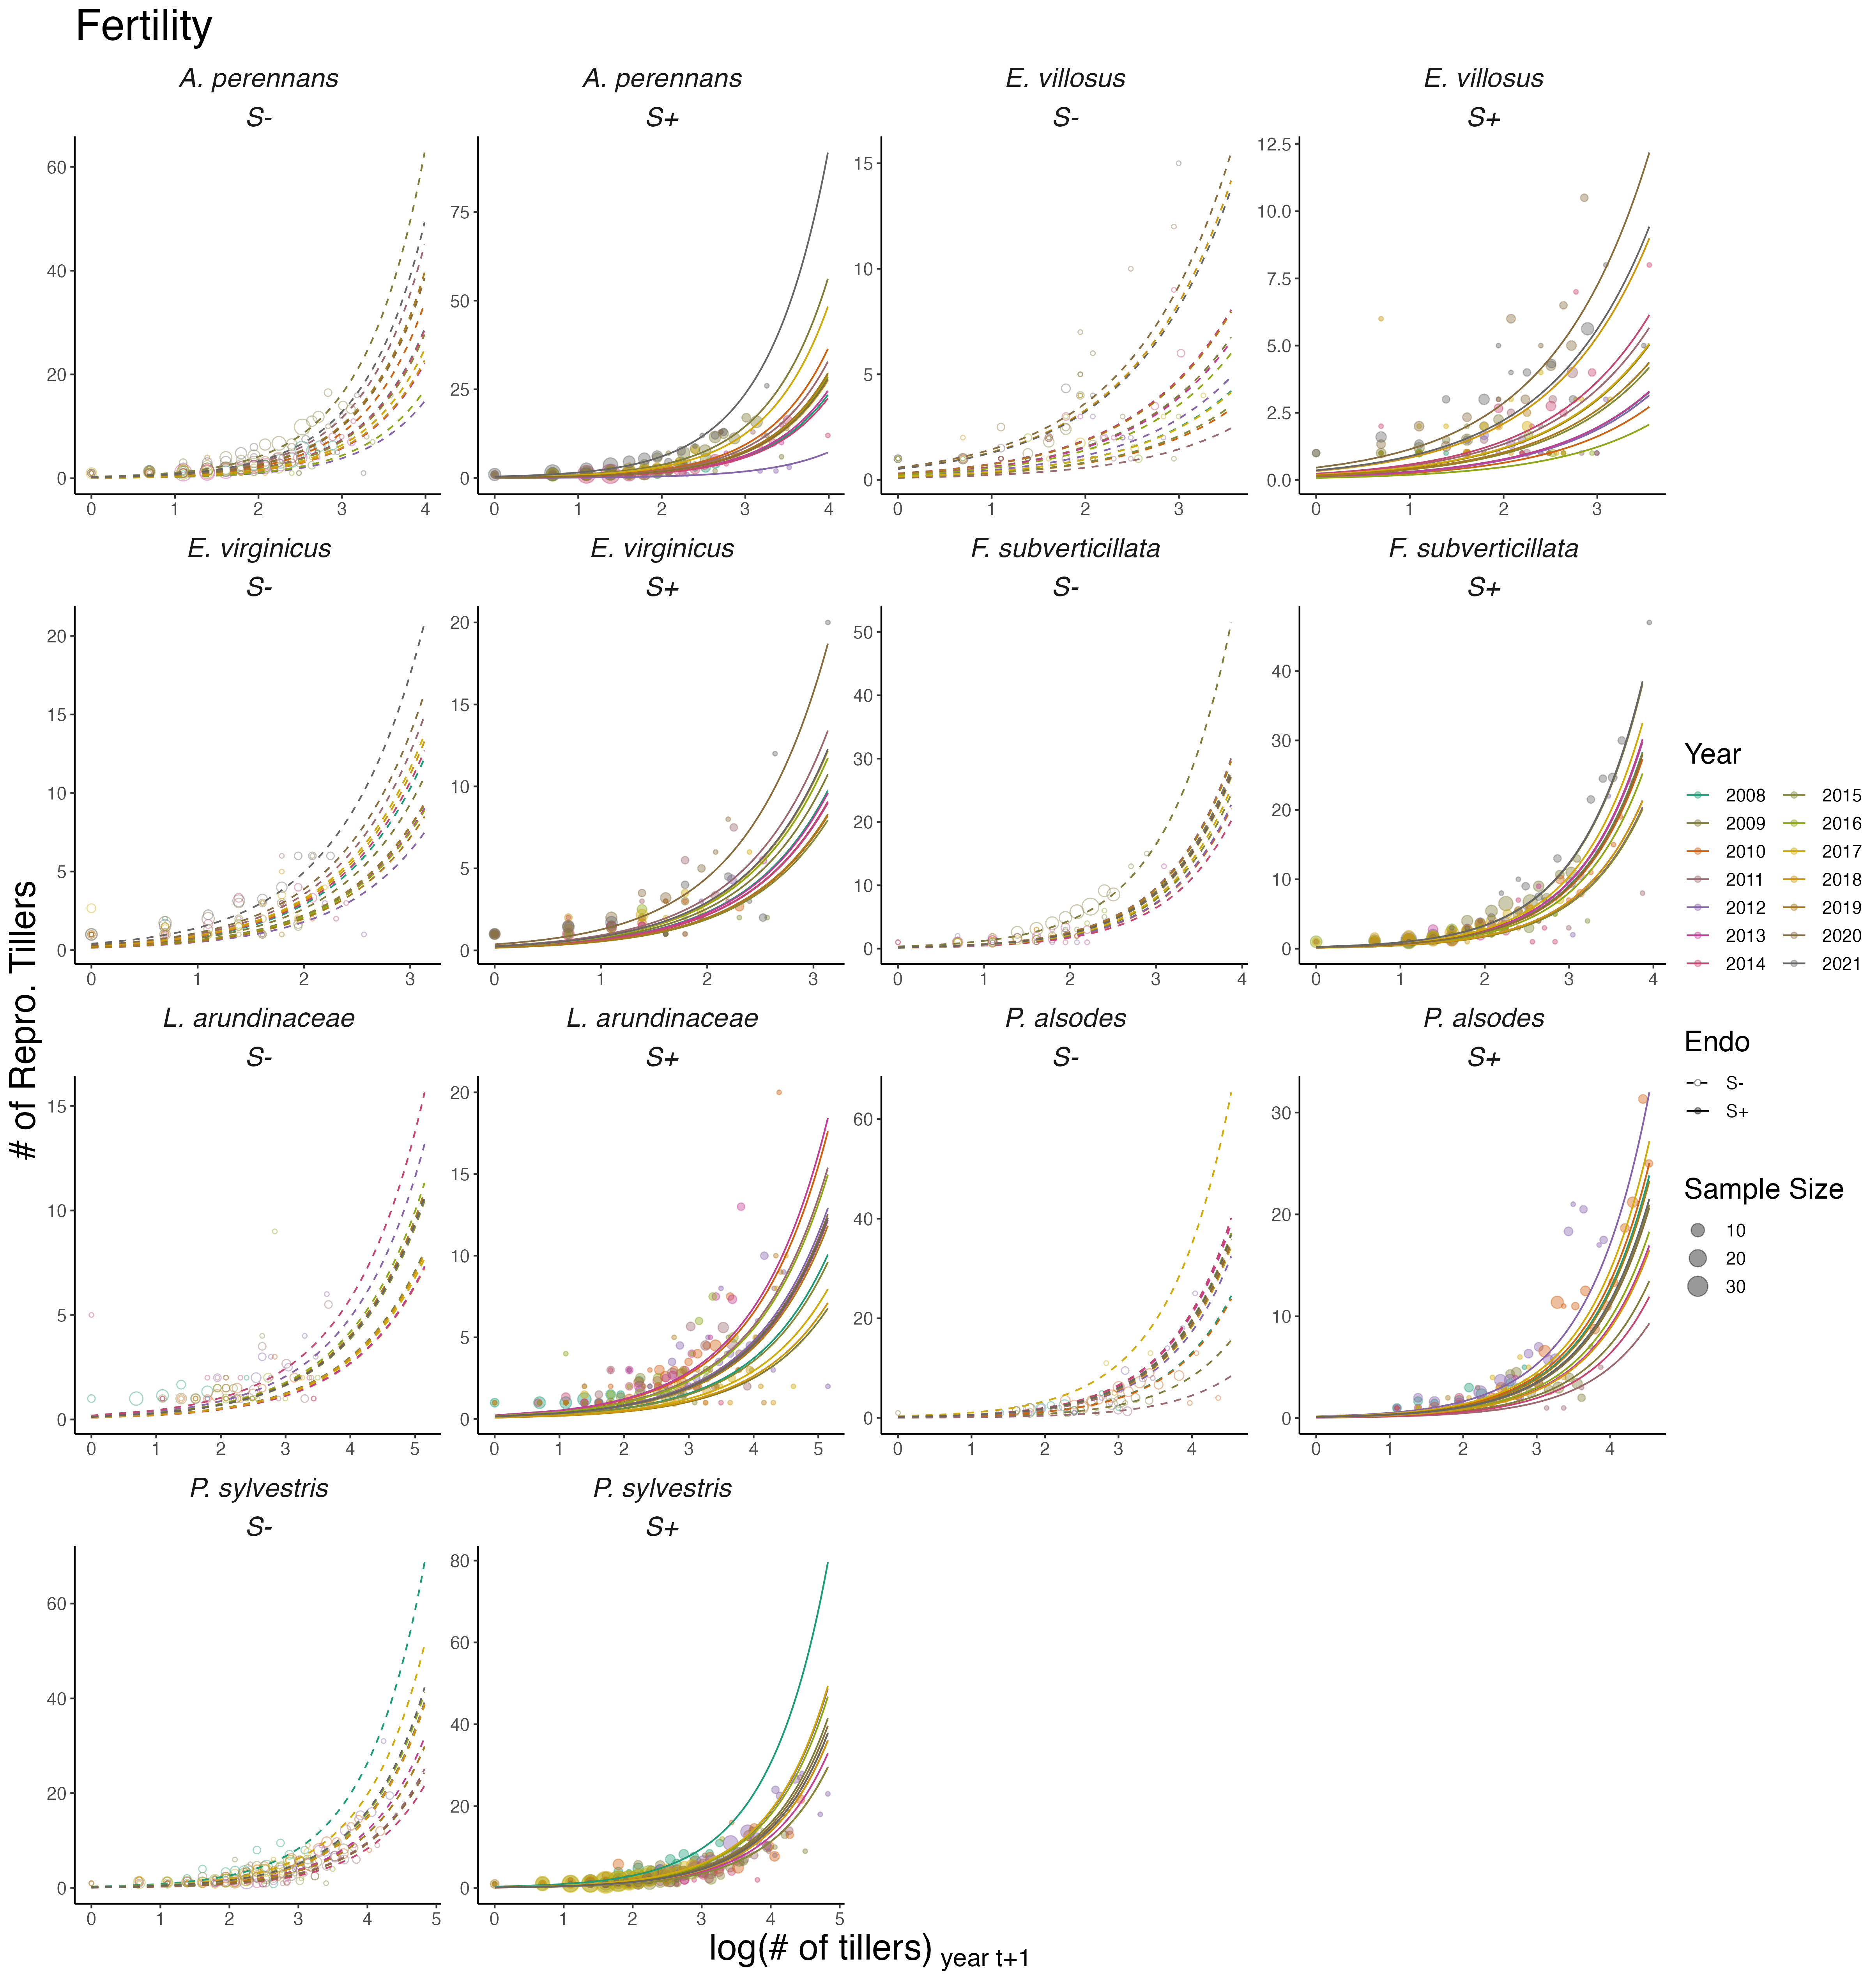
\includegraphics[width=\linewidth]{fert_yearplot.png}
	\caption{Effect of endophyte symbiosis on yearly fertility. Fitted curves represent the size-specific annual expected number of flowering tillers along with data binned by size and census year shown as open circles with a dashed line for symbiont-free (S-) plants, while the solid line and filled circles represent symbiontic (S+) plants.}
\end{figure}


\begin{figure}
	\centering
	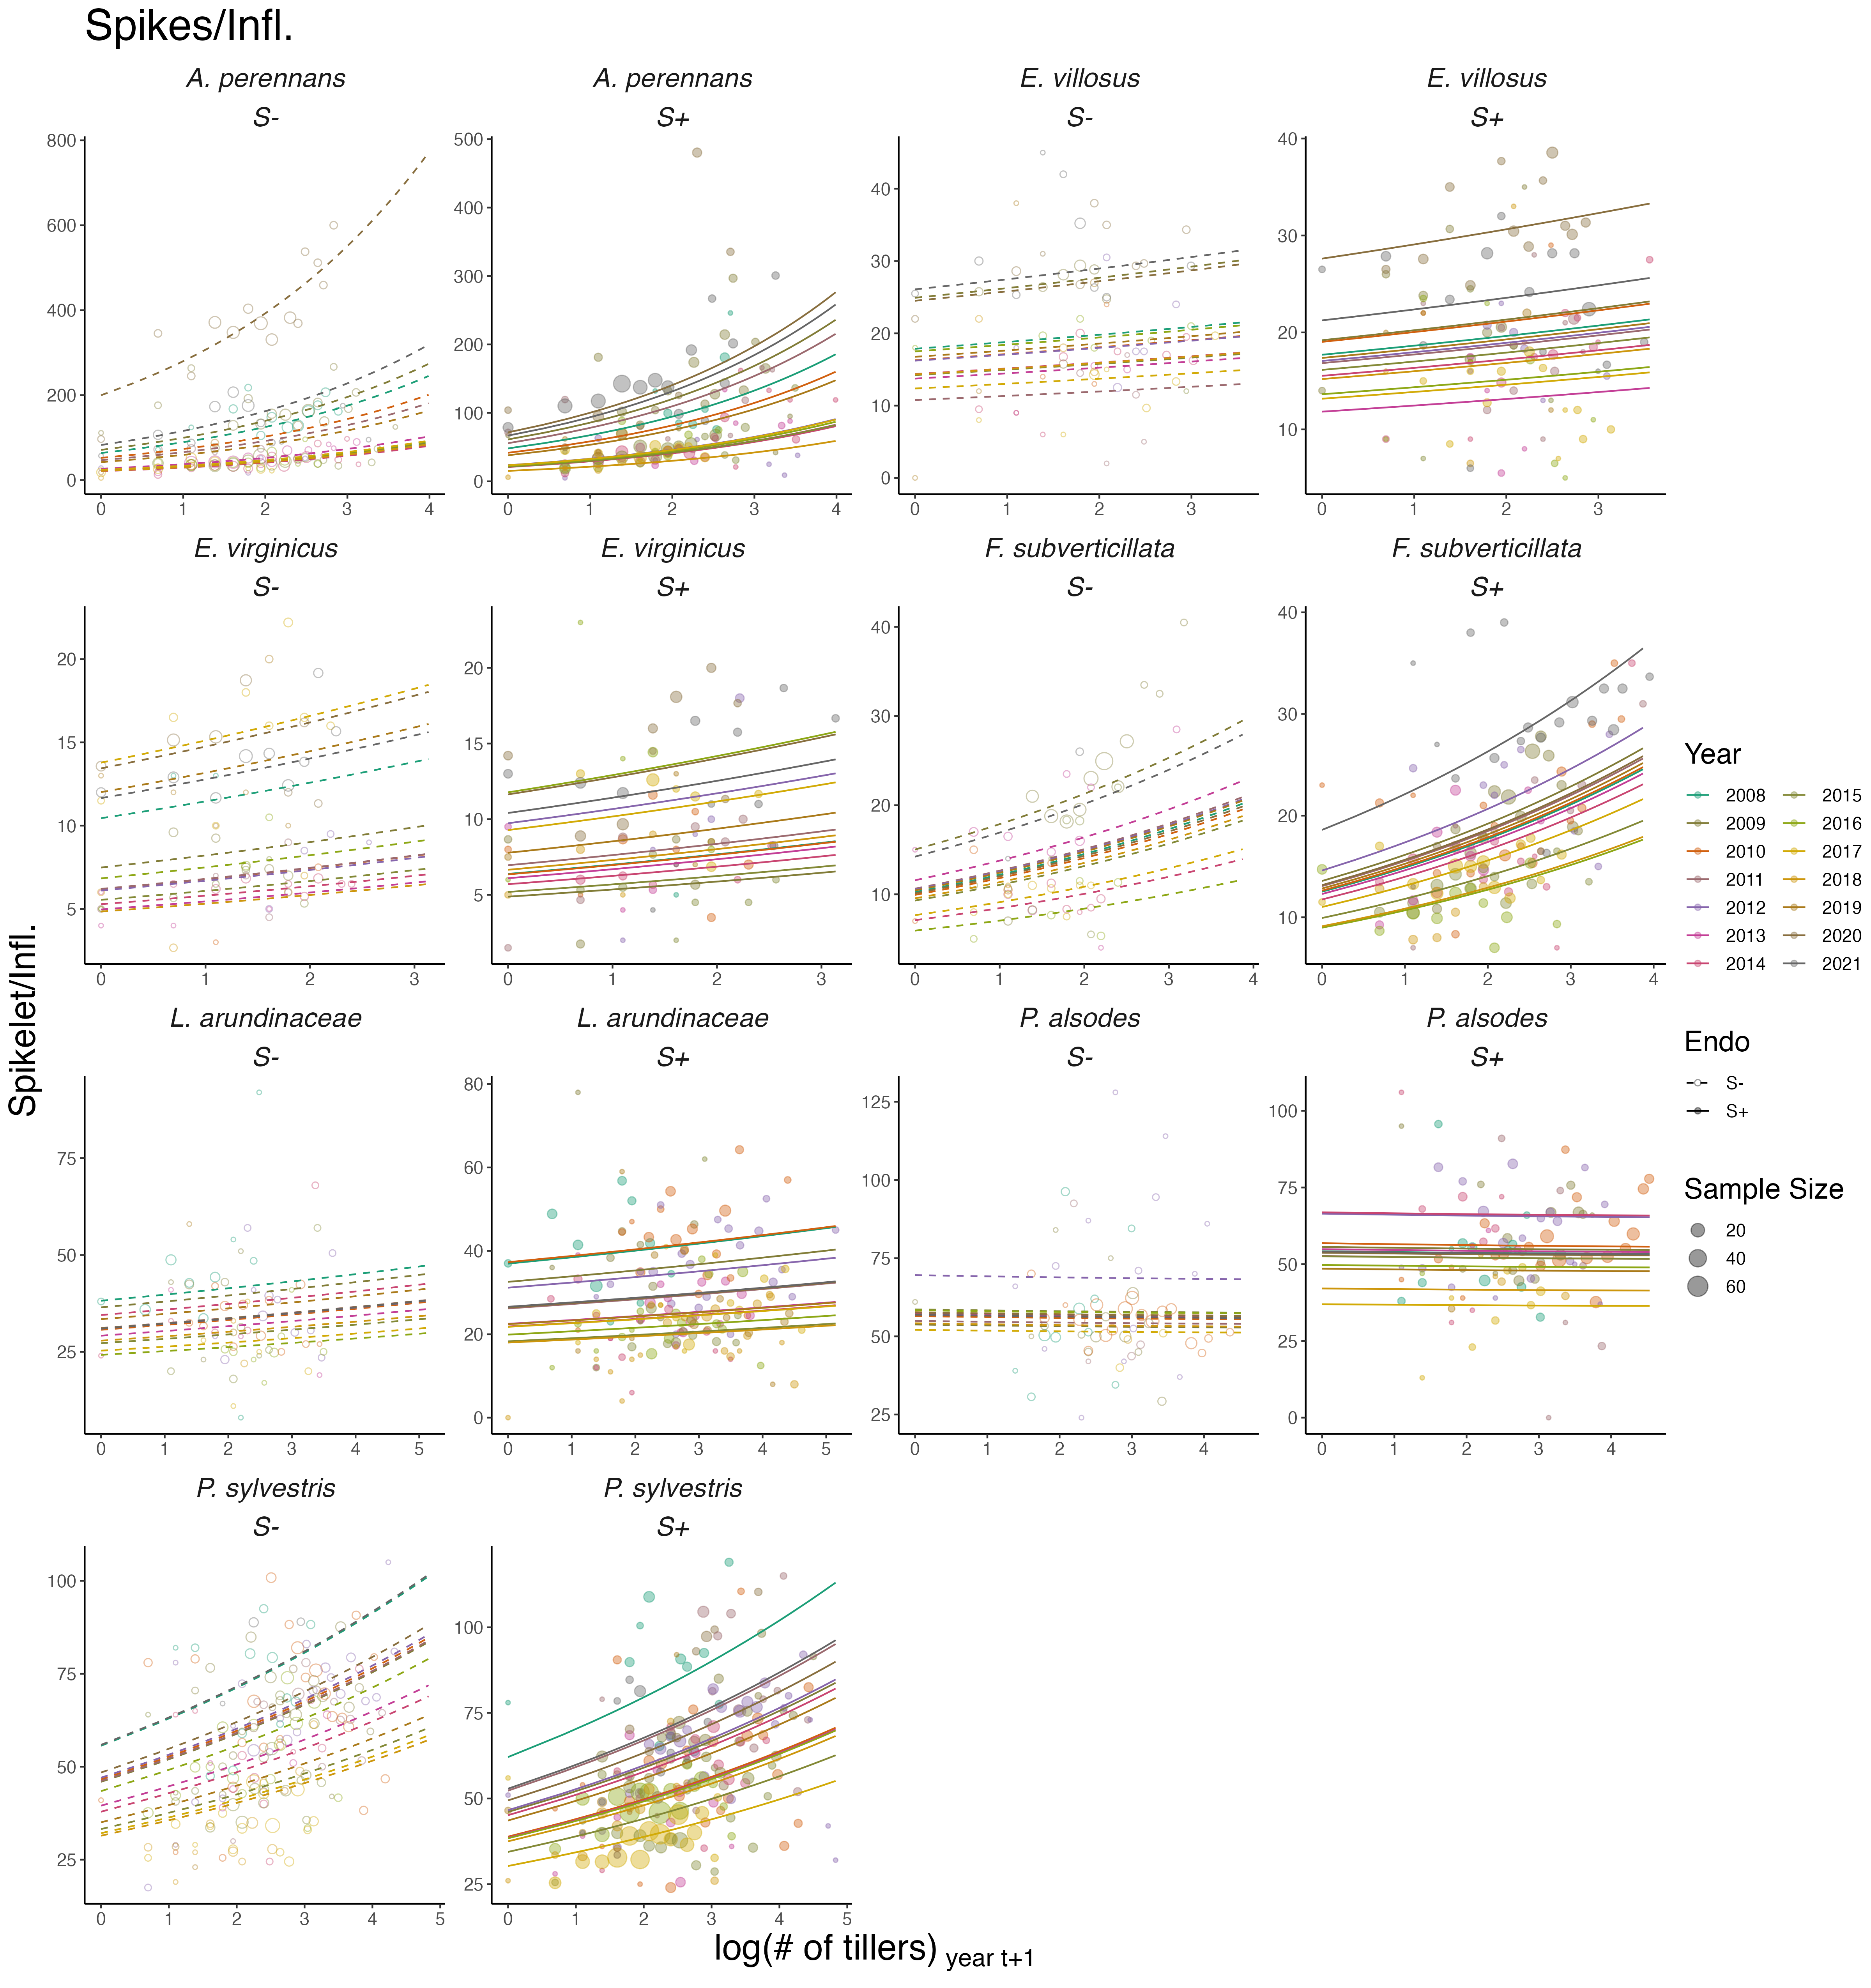
\includegraphics[width=\linewidth]{spike_yearplot.png}
	\caption{Effect of endophyte symbiosis on yearly spikelet production. Fitted curves represent the size-specific annual expected number of spikelets per inflorescence along with data binned by size and census year shown as open circles with a dashed line for symbiont-free (S-) plants, while the solid line and filled circles represent symbiontic (S+) plants.}
\end{figure}


\begin{figure}
	\centering
	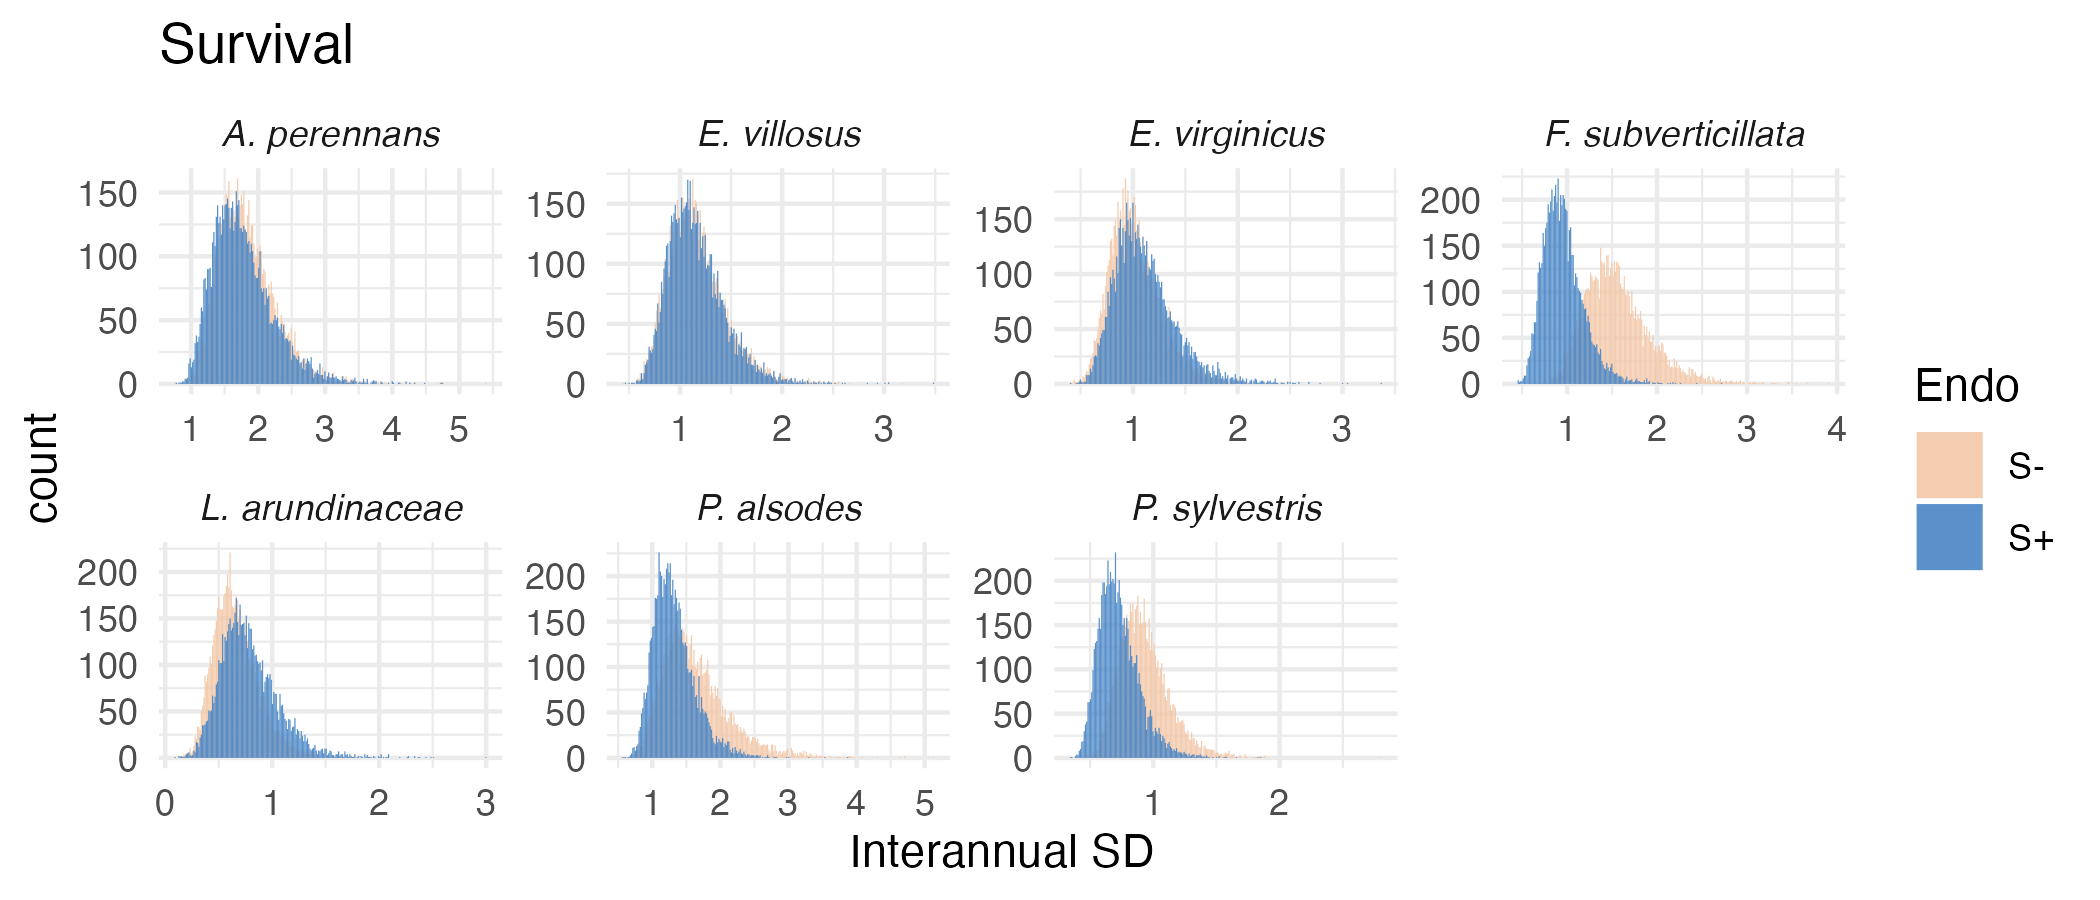
\includegraphics[width=.9\linewidth]{surv_sigmayear_hist.png}
	\caption{Posterior distributions of the standard deviations of inter-annual year effects for survival. Histograms include 7500 post-warmup MCMC samples for symbiotic (S+; blue) and symbiont-free (S-; tan) plants from fitted vital rate model.}
\end{figure}

\newpage

\begin{figure}
	\centering
	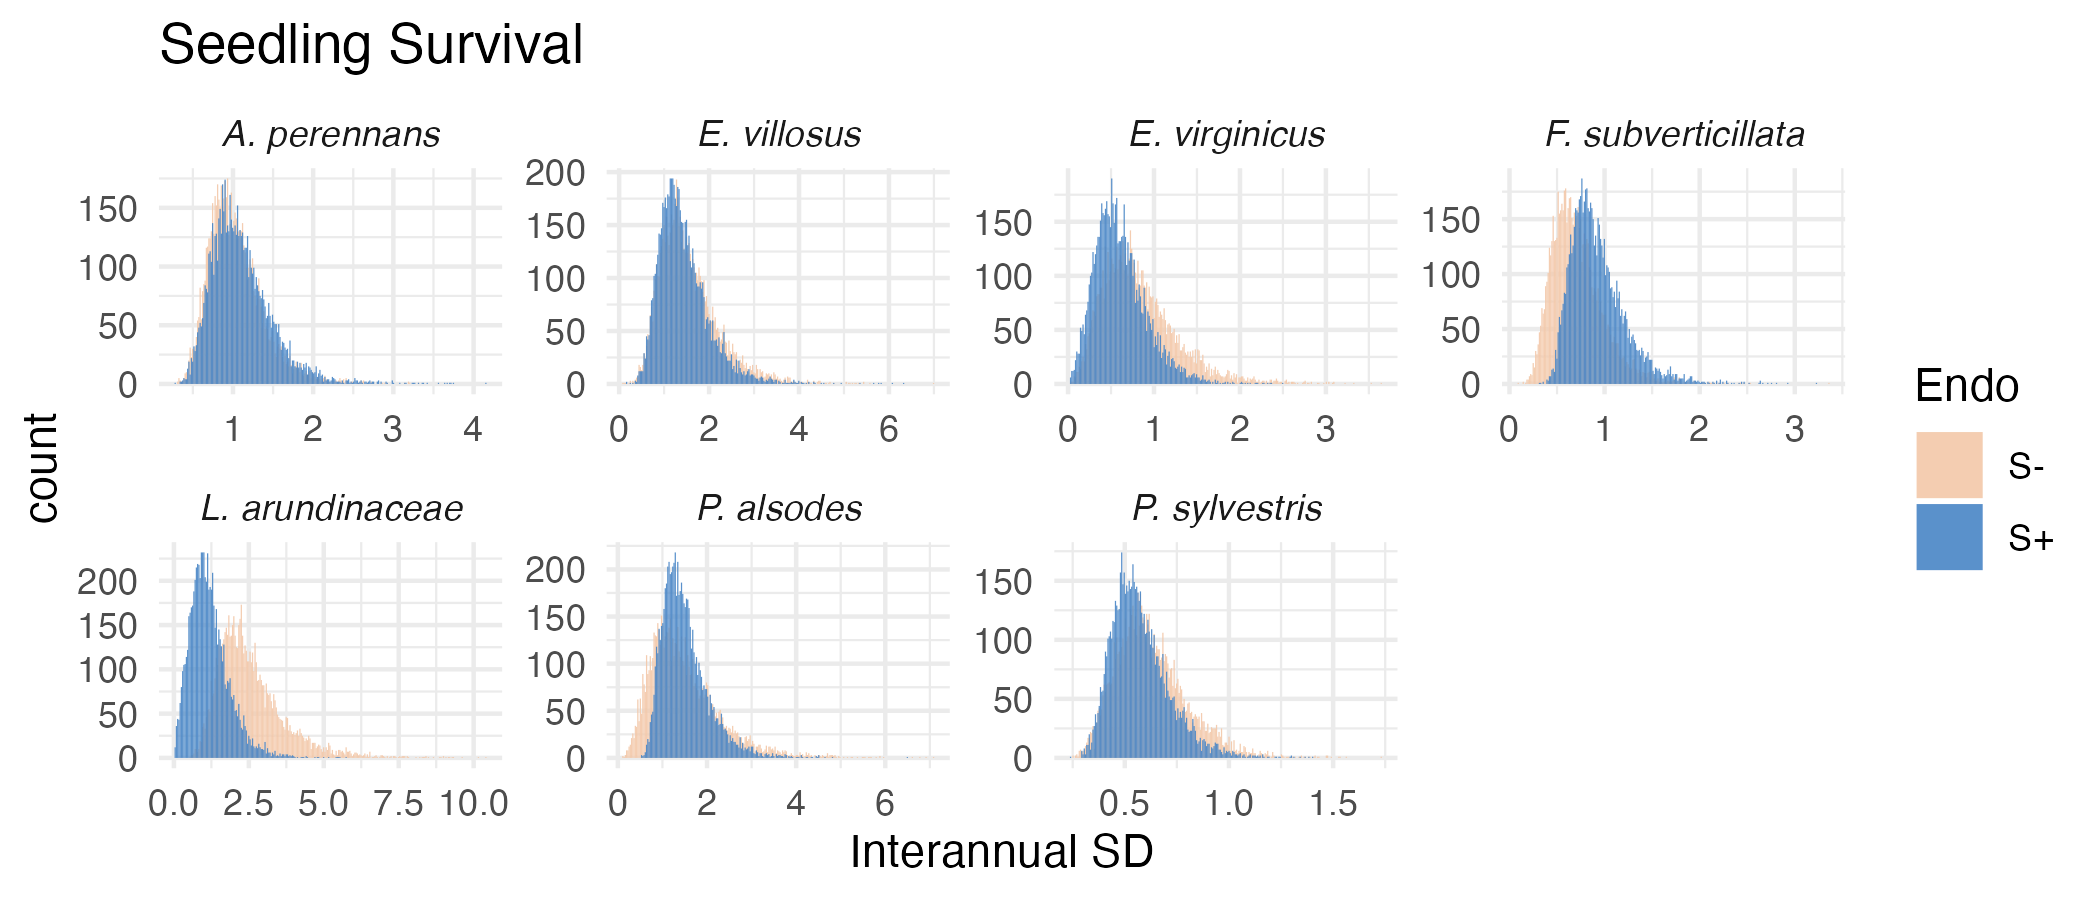
\includegraphics[width=.9\linewidth]{seedsurv_sigmayear_hist.png}
	\caption{Posterior distributions of the standard deviations of inter-annual year effects for seedling survival. Histograms include 7500 post-warmup MCMC samples for symbiotic (S+; blue) and symbiont-free (S-; tan) plants from fitted vital rate model.}
\end{figure}

\newpage

\begin{figure}
	\centering
	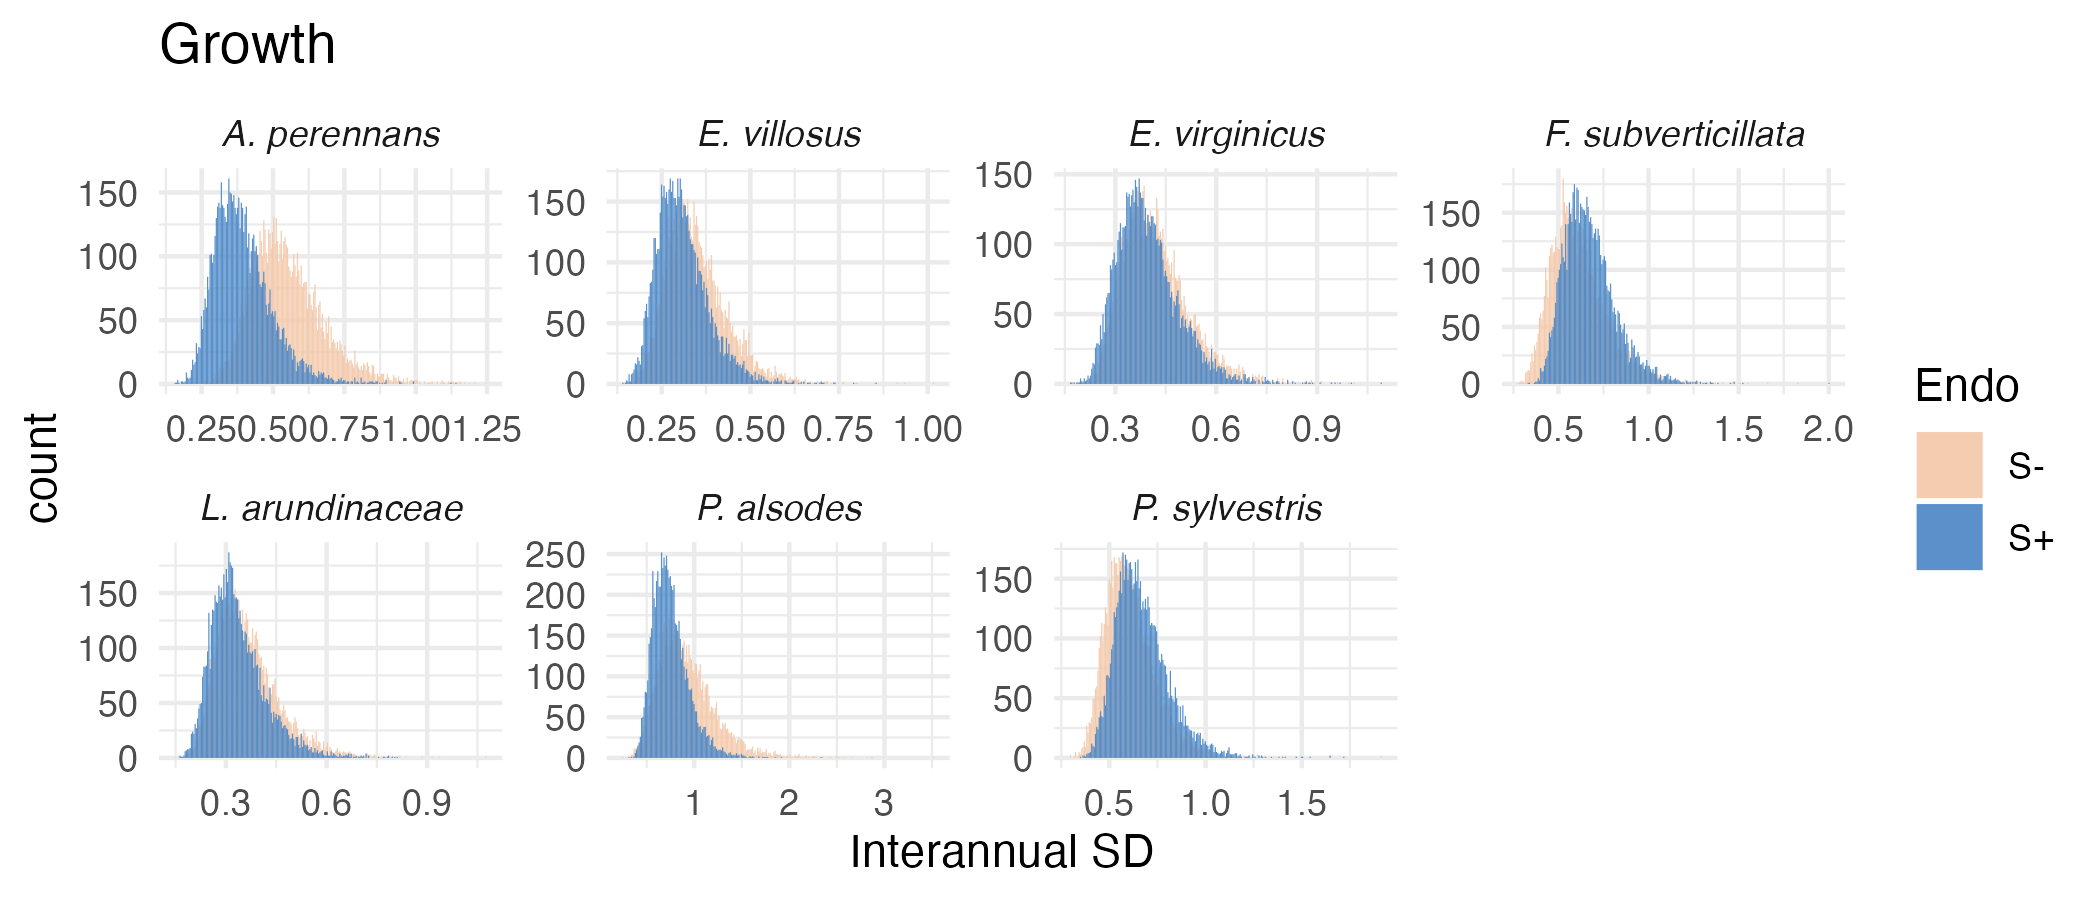
\includegraphics[width=.9\linewidth]{grow_sigmayear_hist.png}
	\caption{Posterior distributions of the standard deviations of inter-annual year effects for growth. Histograms include 7500 post-warmup MCMC samples for symbiotic (S+; blue) and symbiont-free (S-; tan) plants from fitted vital rate model.}
\end{figure}
\newpage

\begin{figure}
	\centering
	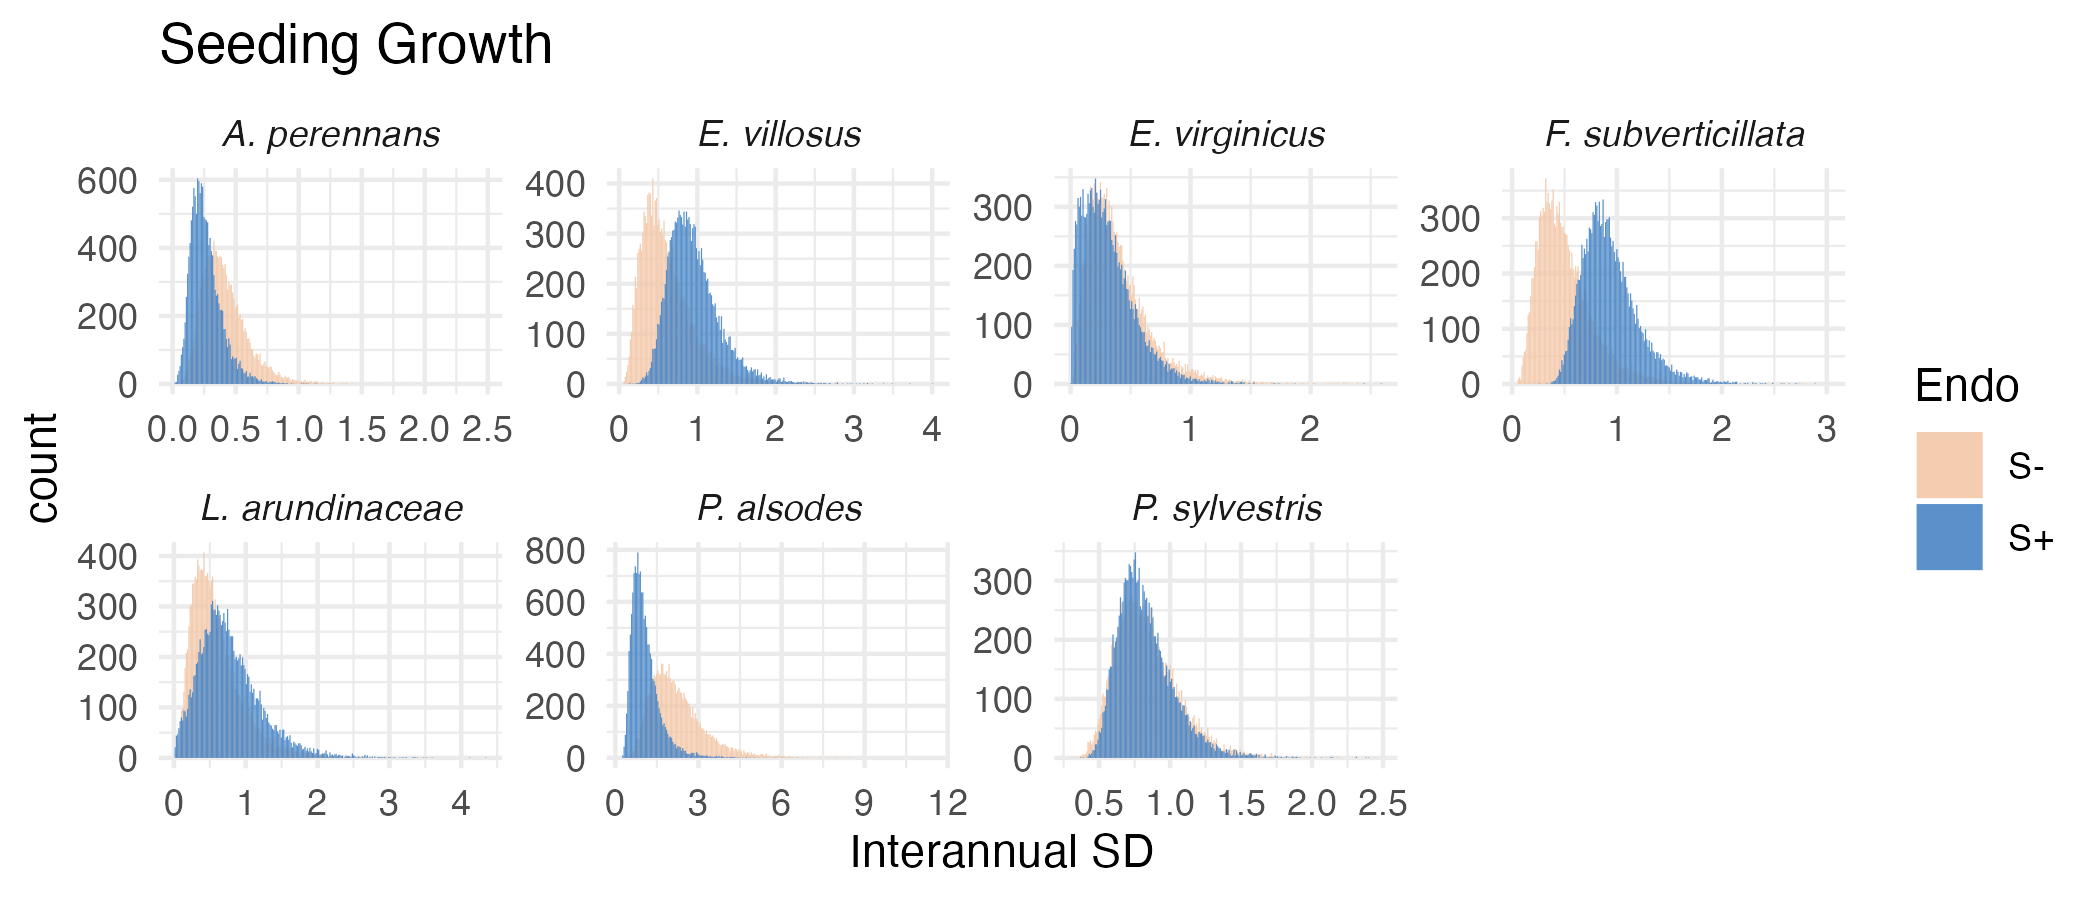
\includegraphics[width=.9\linewidth]{seedgrow_sigmayear_hist.png}
	\caption{Posterior distributions of the standard deviations of inter-annual year effects for seedling growth. Histograms include 7500 post-warmup MCMC samples for symbiotic (S+; blue) and symbiont-free (S-; tan) plants from fitted vital rate model.}
\end{figure}

\newpage
\begin{figure}
	\centering
	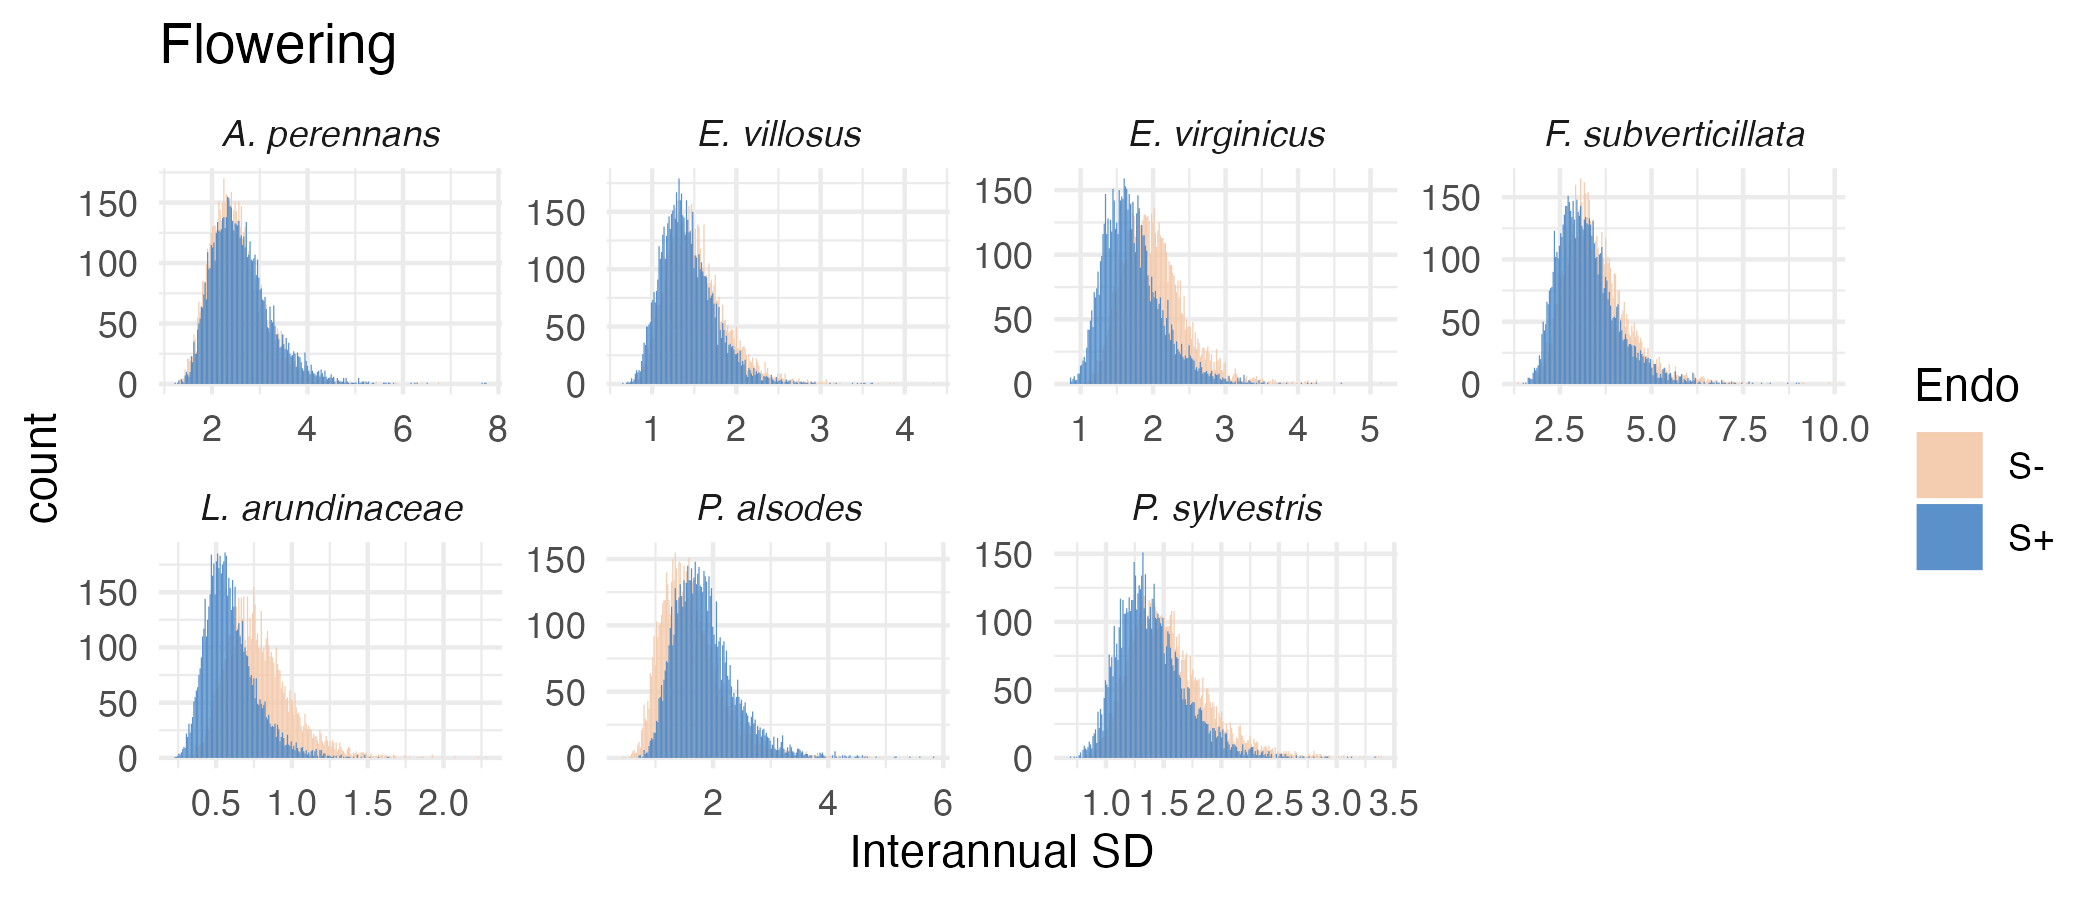
\includegraphics[width=.9\linewidth]{flow_sigmayear_hist.png}
	\caption{Posterior distributions of the standard deviations of inter-annual year effects for flowering probability. Histograms include 7500 post-warmup MCMC samples for symbiotic (S+; blue) and symbiont-free (S-; tan) plants from fitted vital rate model.}
\end{figure}

\newpage
\begin{figure}
	\centering
	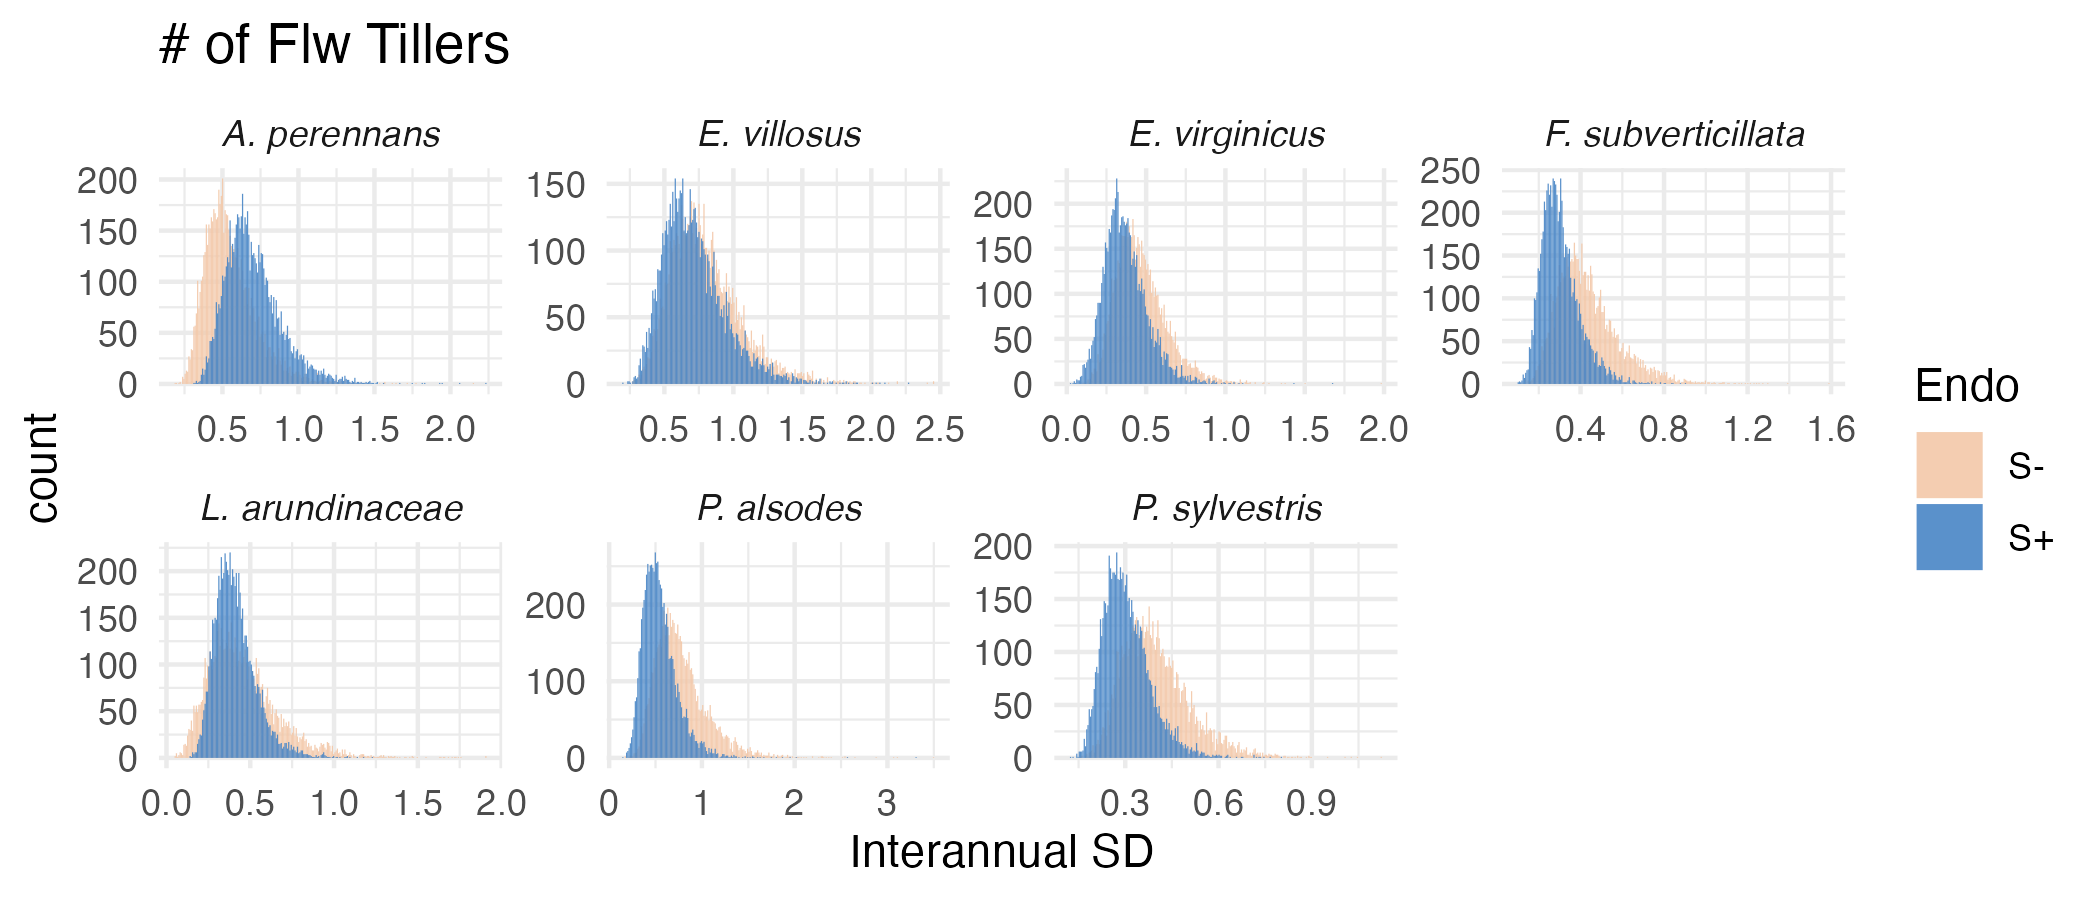
\includegraphics[width=.9\linewidth]{fert_sigmayear_hist.png}
	\caption{Posterior distributions of the standard deviations of inter-annual year effects for fertility (no. of flowering tillers). Histograms include 7500 post-warmup MCMC samples for symbiotic (S+; blue) and symbiont-free (S-; tan) plants from fitted vital rate model.}
\end{figure}

\newpage
\begin{figure}
	\centering
	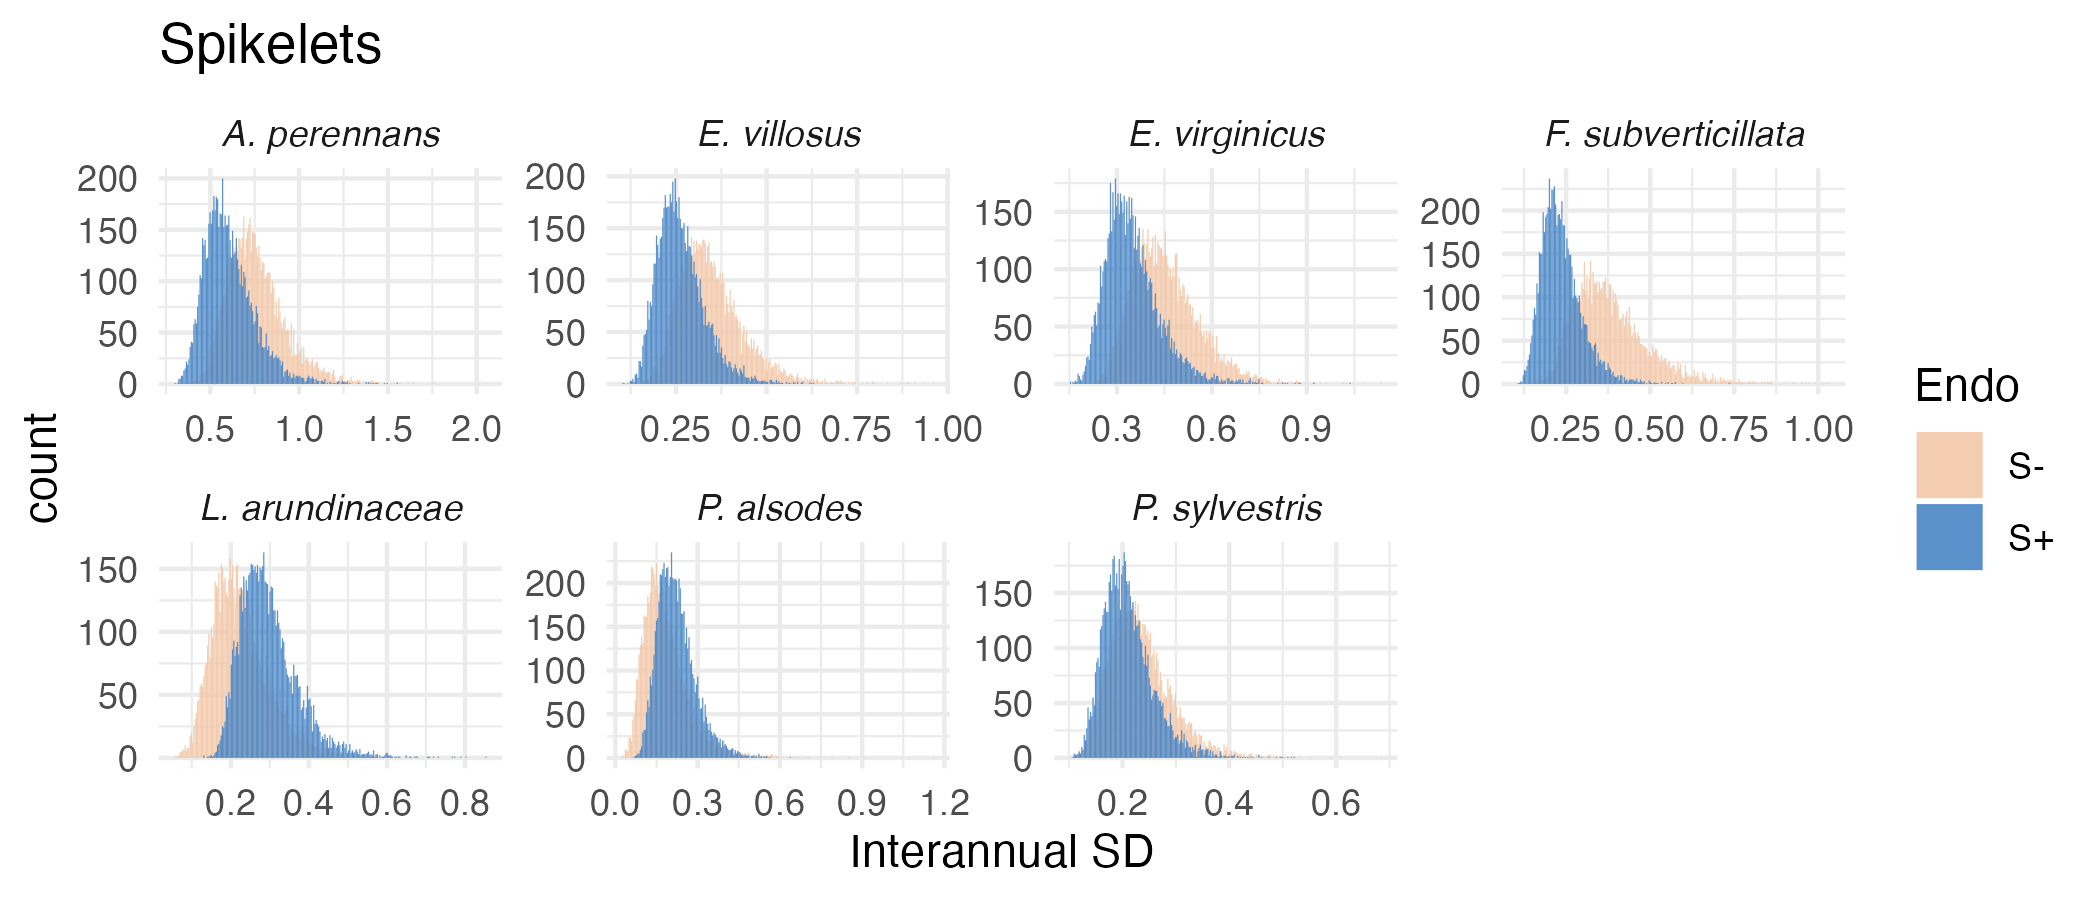
\includegraphics[width=.9\linewidth]{spike_sigmayear_hist.png}
	\caption{Posterior distributions of the standard deviations of inter-annual year effects for spikelets per inflorescence. Histograms include 7500 post-warmup MCMC samples for symbiotic (S+; blue) and symbiont-free (S-; tan) plants from fitted vital rate model.}
\end{figure}
\newpage

\begin{figure}
	\centering
	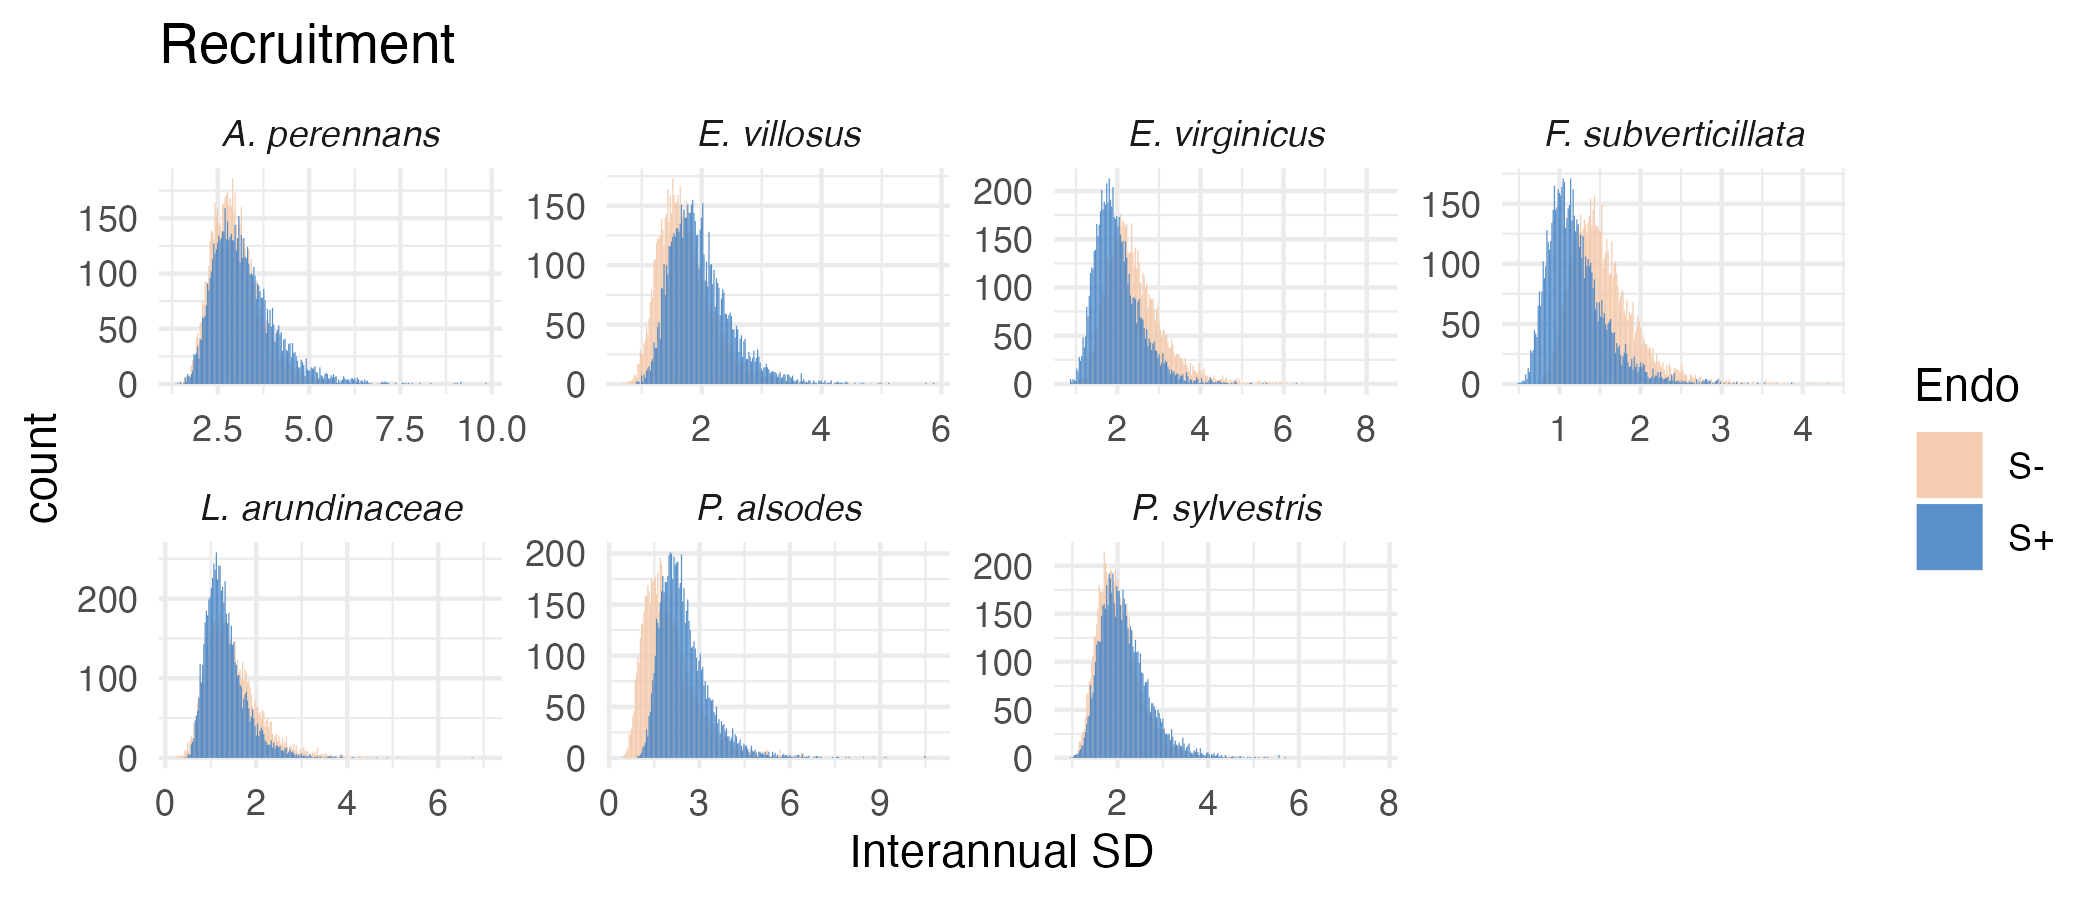
\includegraphics[width=.9\linewidth]{recruit_sigmayear_hist.png}
	\caption{Posterior distributions of the standard deviations of inter-annual year effects for recruitment. Histograms include 7500 post-warmup MCMC samples for symbiotic (S+; blue) and symbiont-free (S-; tan) plants from fitted vital rate model.}
\end{figure}
\newpage

\begin{figure}
	\centering
	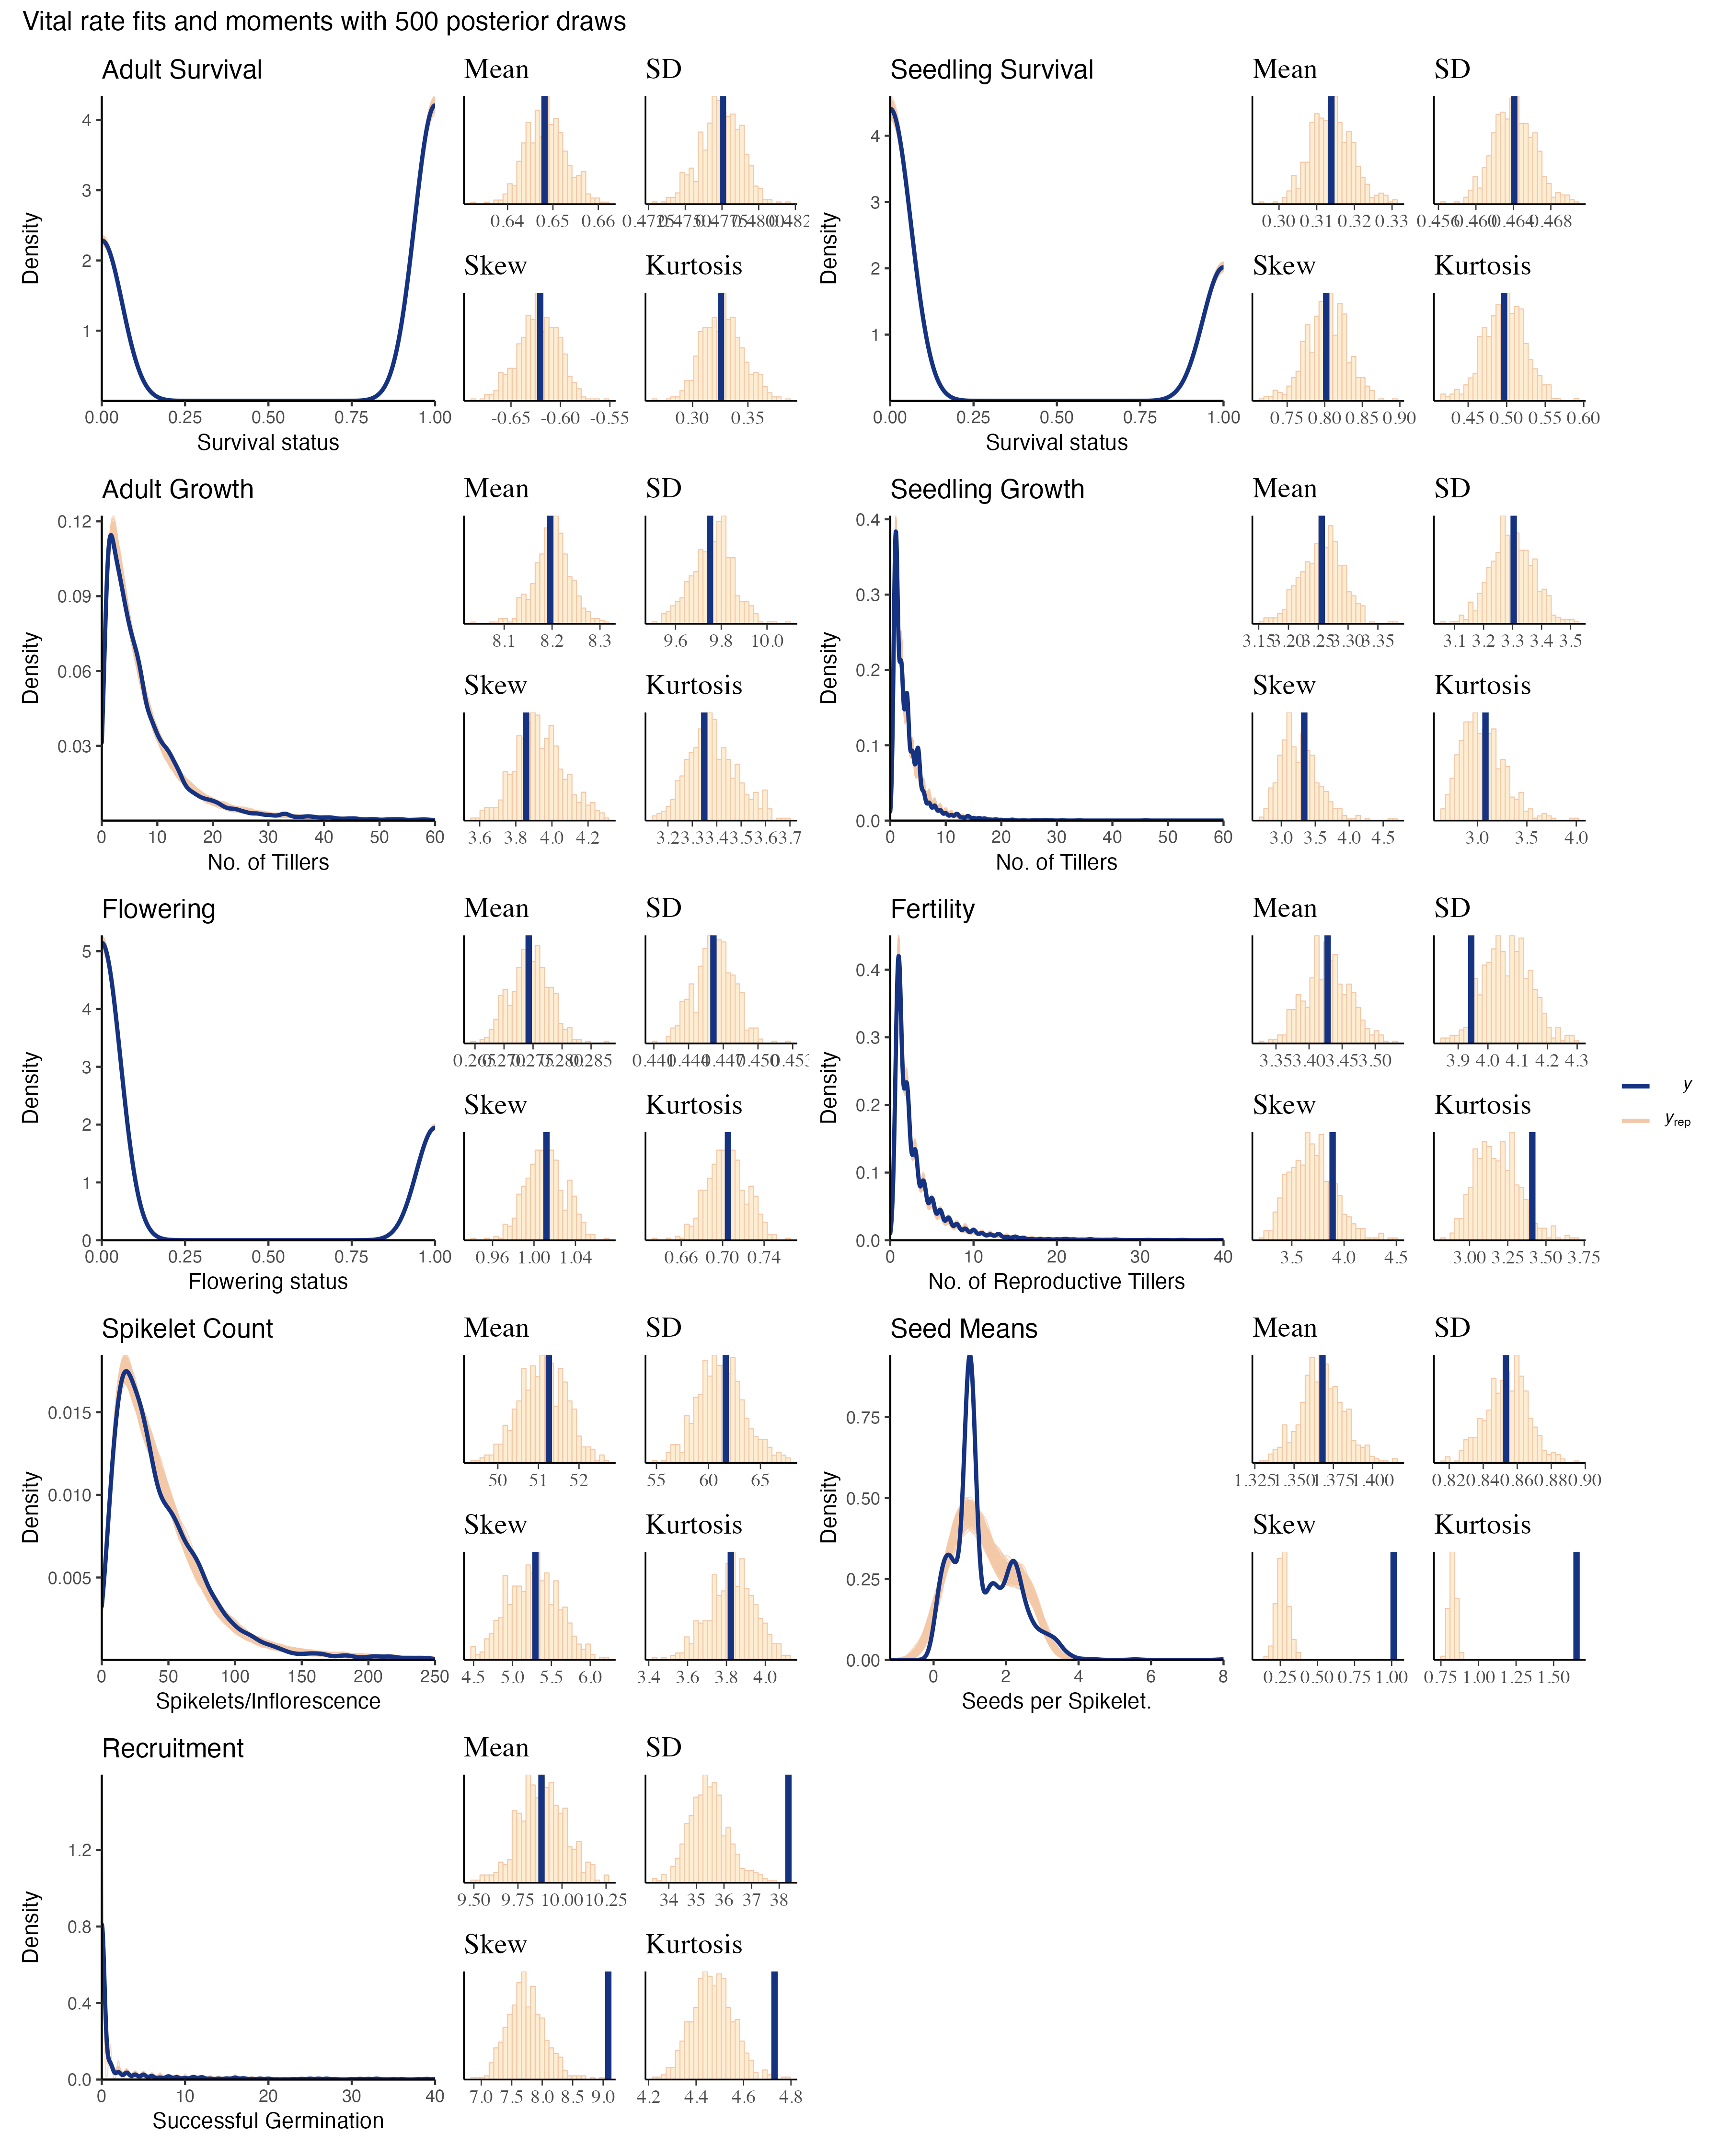
\includegraphics[width=.7\linewidth]{fitsandmoments_plot.png}
	\caption{Consistency between real data and simulated values indicates that fitted models describe the data well. Graphs show posterior predictive check for statistical models of demographic vital rates. Lines show density distributions of observed data (blue line) compared to data simulated from fitted models (tan lines) generated from 500 draws from posterior distributions of model parameters.}
\end{figure}

\newpage
\begin{figure}
	\centering
	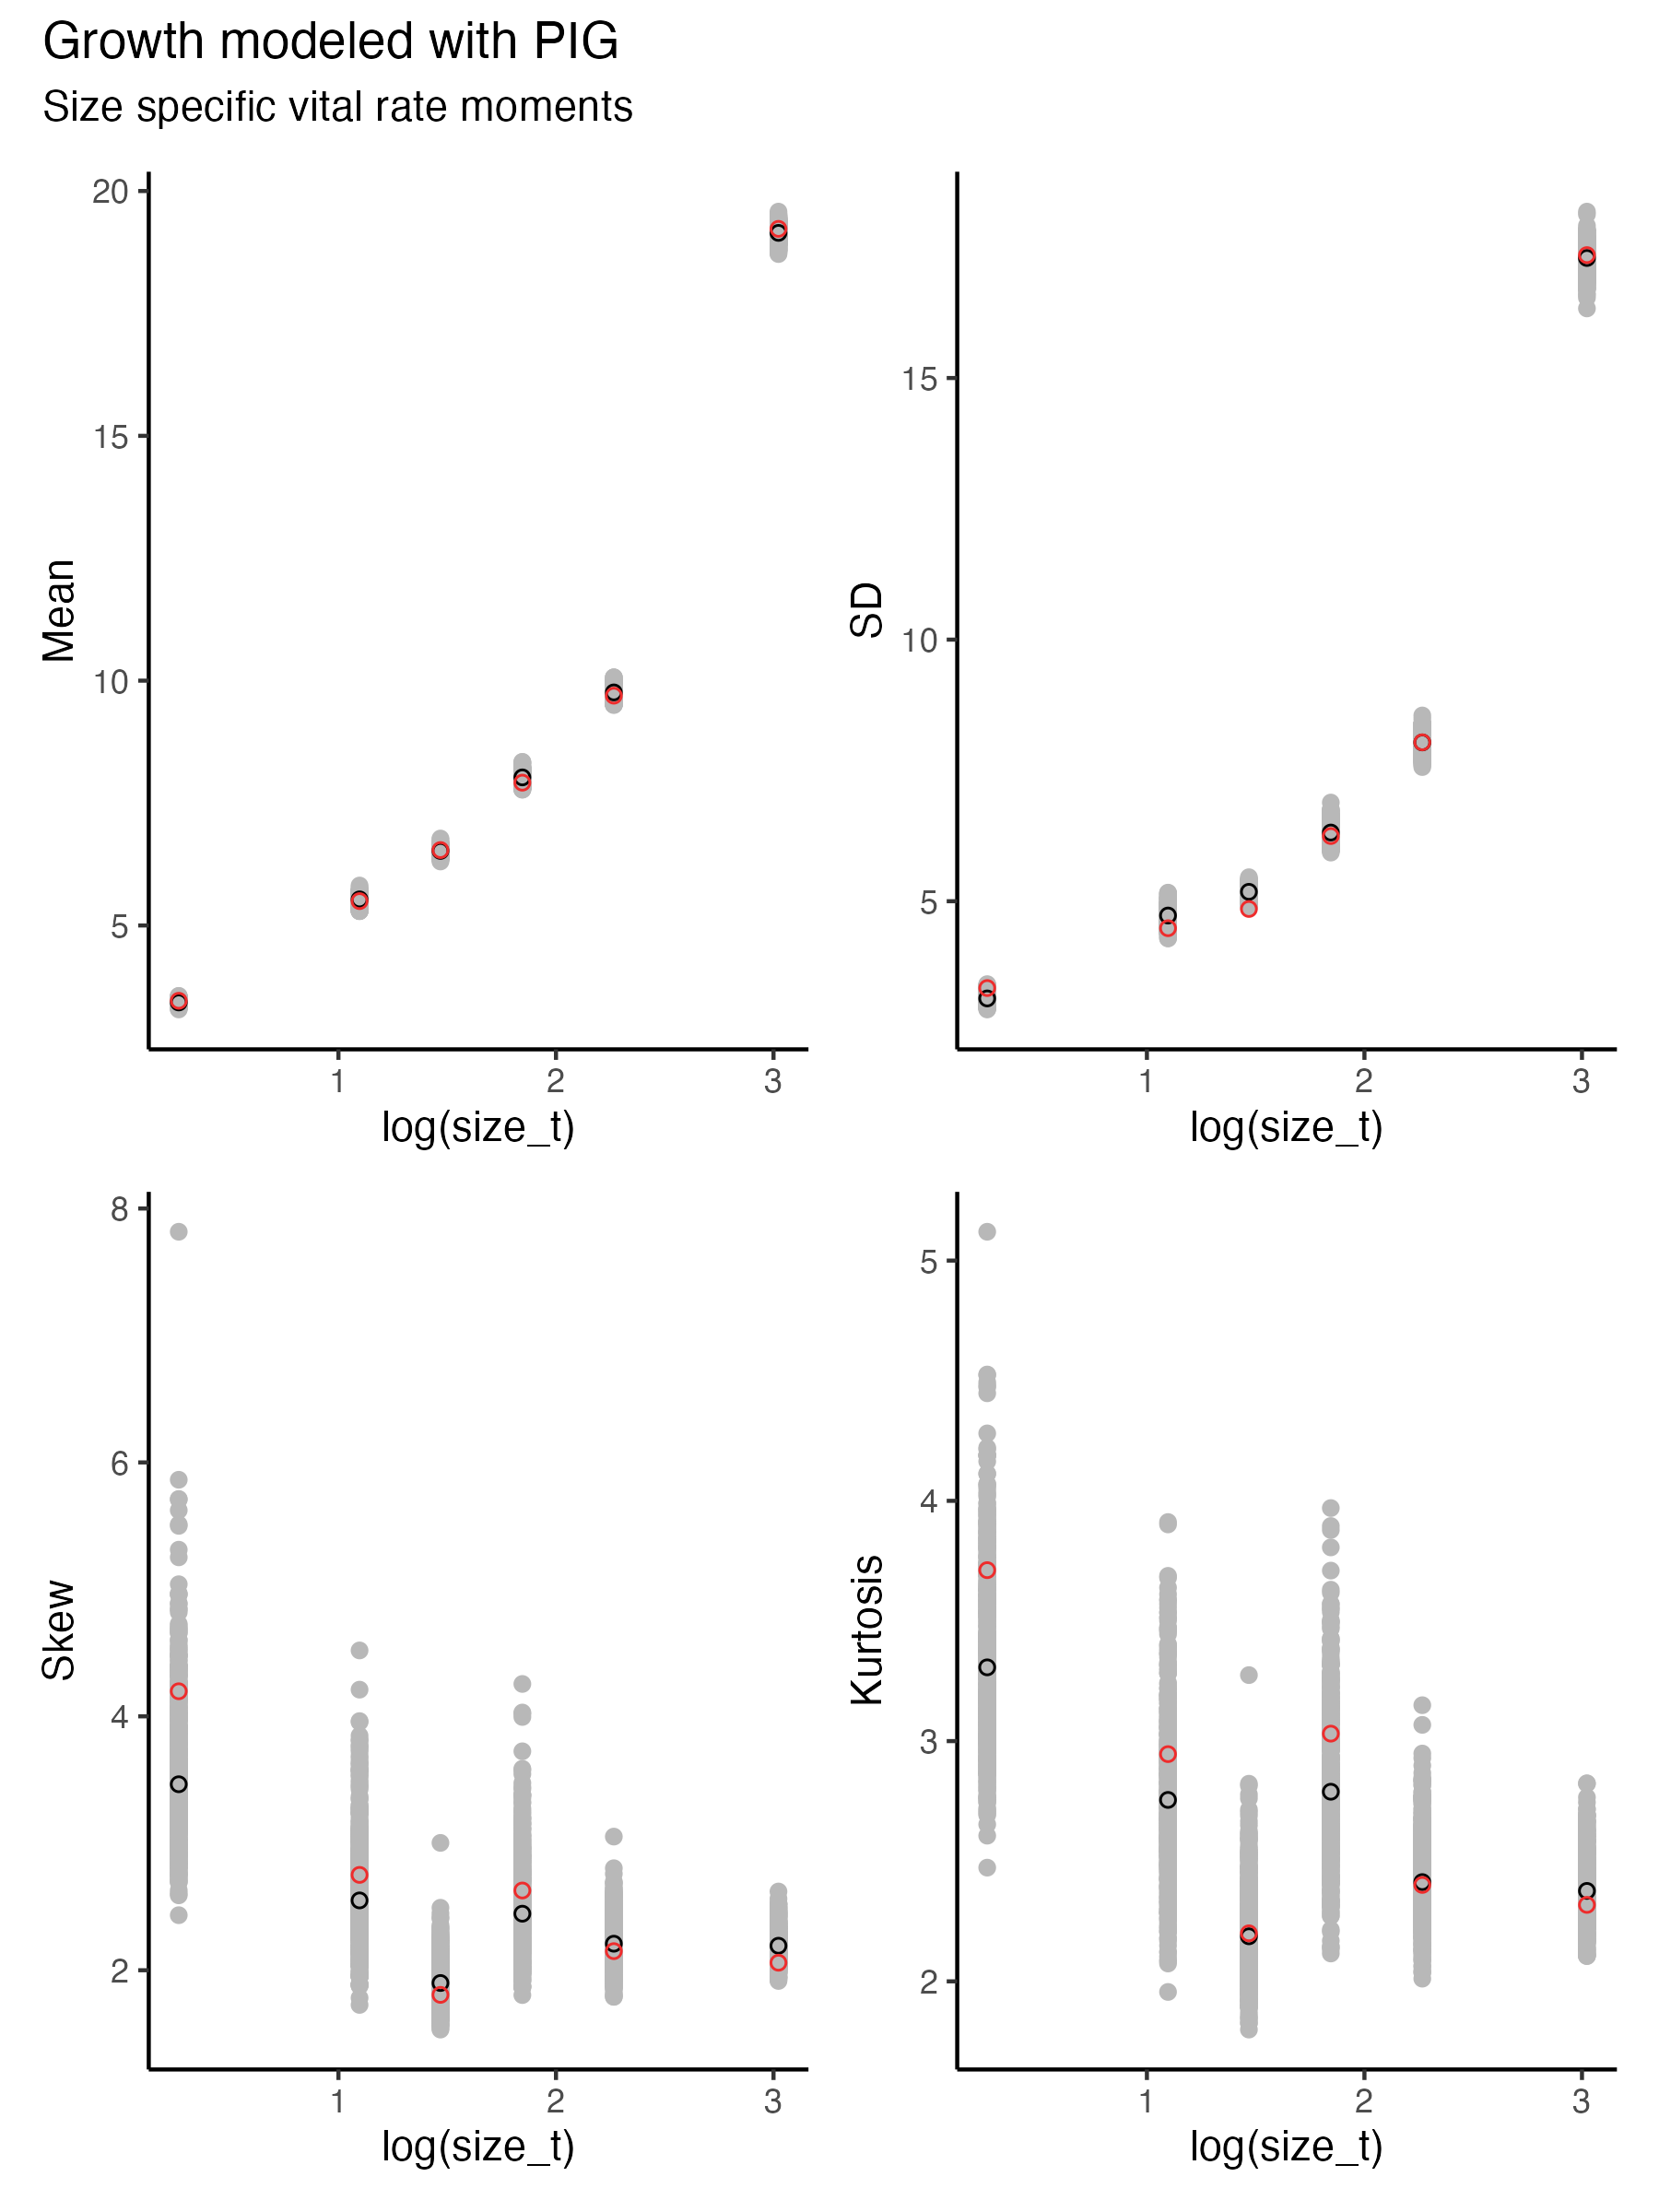
\includegraphics[width=.6\linewidth]{size_ppc_plot.png}
	\caption{Consistency between real data and fitted values across sizes indicates that the growth model is accurately capturing size dependence. Graphs of posterior predictive check for mean and higher moments of the growth model across size. Points show the value of statistical moments binned across size for the observed data (red circles) compared to the simulated datasets (grey circles) and the median of the simulated values (black circles) generated from 500 posterior draws from the fitted model. }
\end{figure}

\newpage
\begin{figure}
	\centering
	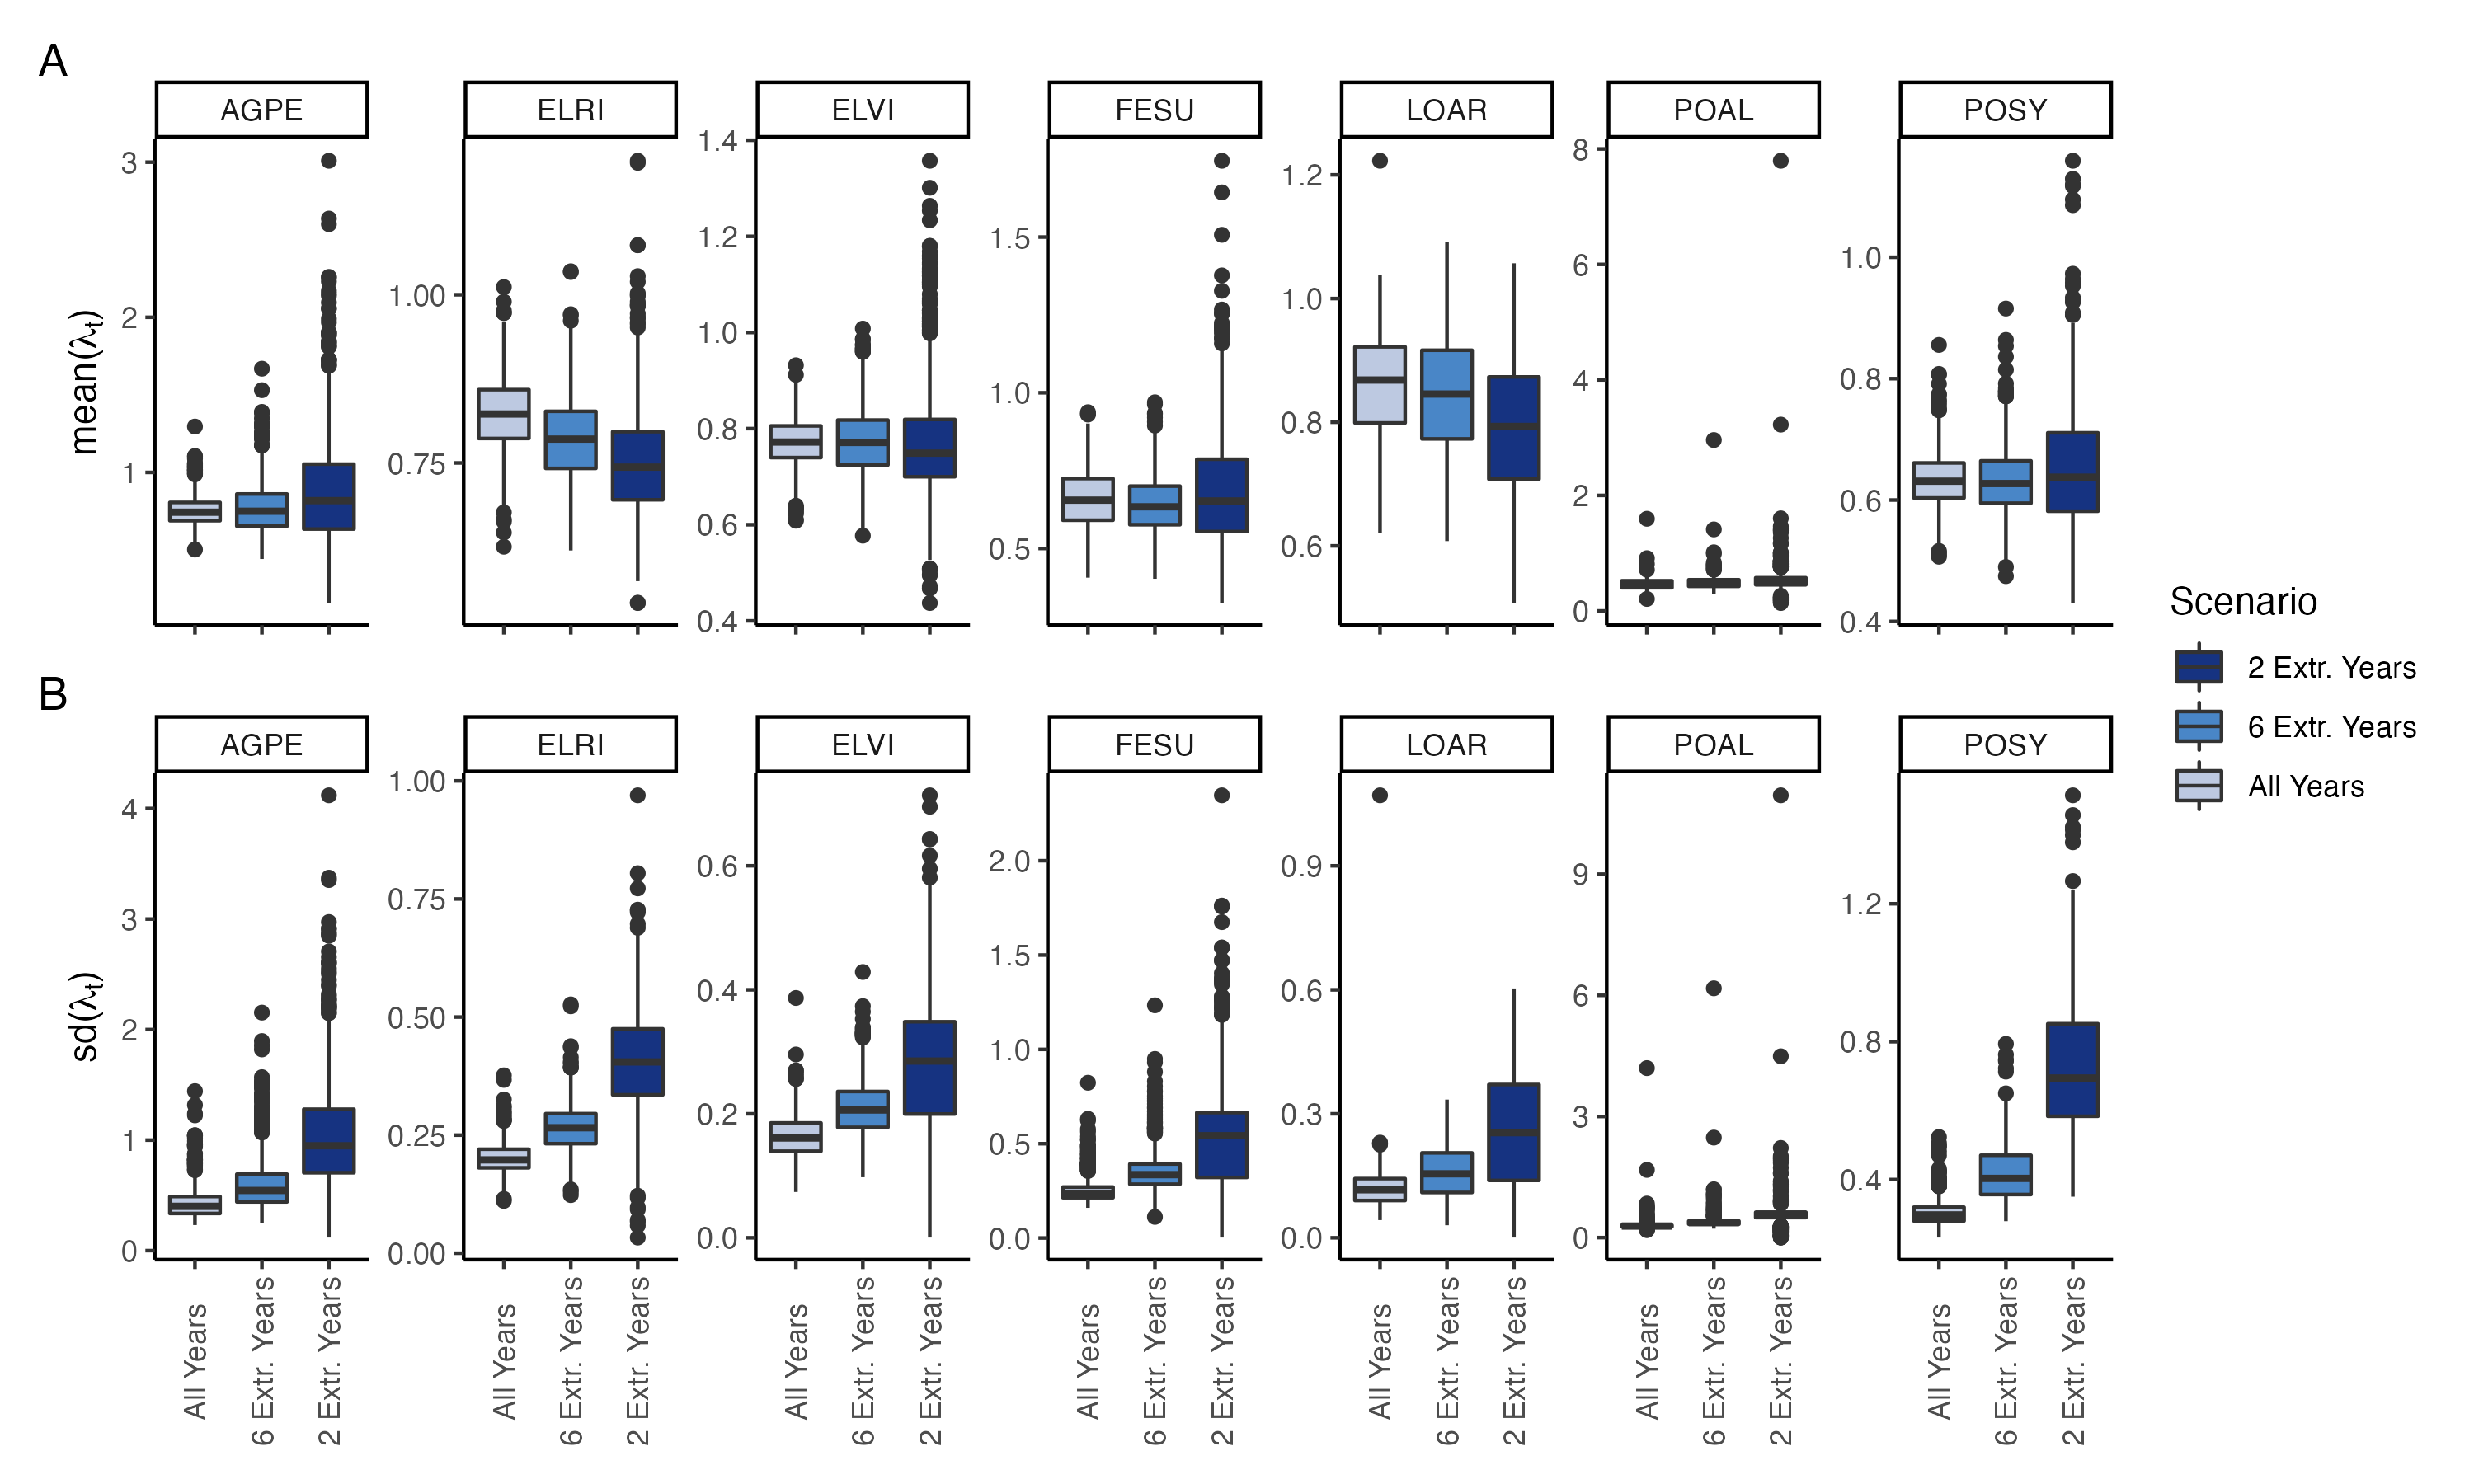
\includegraphics[width=\linewidth]{sim_boxplots.png}
	\caption{(A) Mean and (B) standard deviation of annual growth rate values during simulation scenarios. Each scenario selects from observed transition matrixes, increasing the variance by selecting either all observed years, or a set (6 or 2 years) that have the highest and lowest growth rates for symbiont-free populations.}
\end{figure}


\begin{figure}
	\centering
	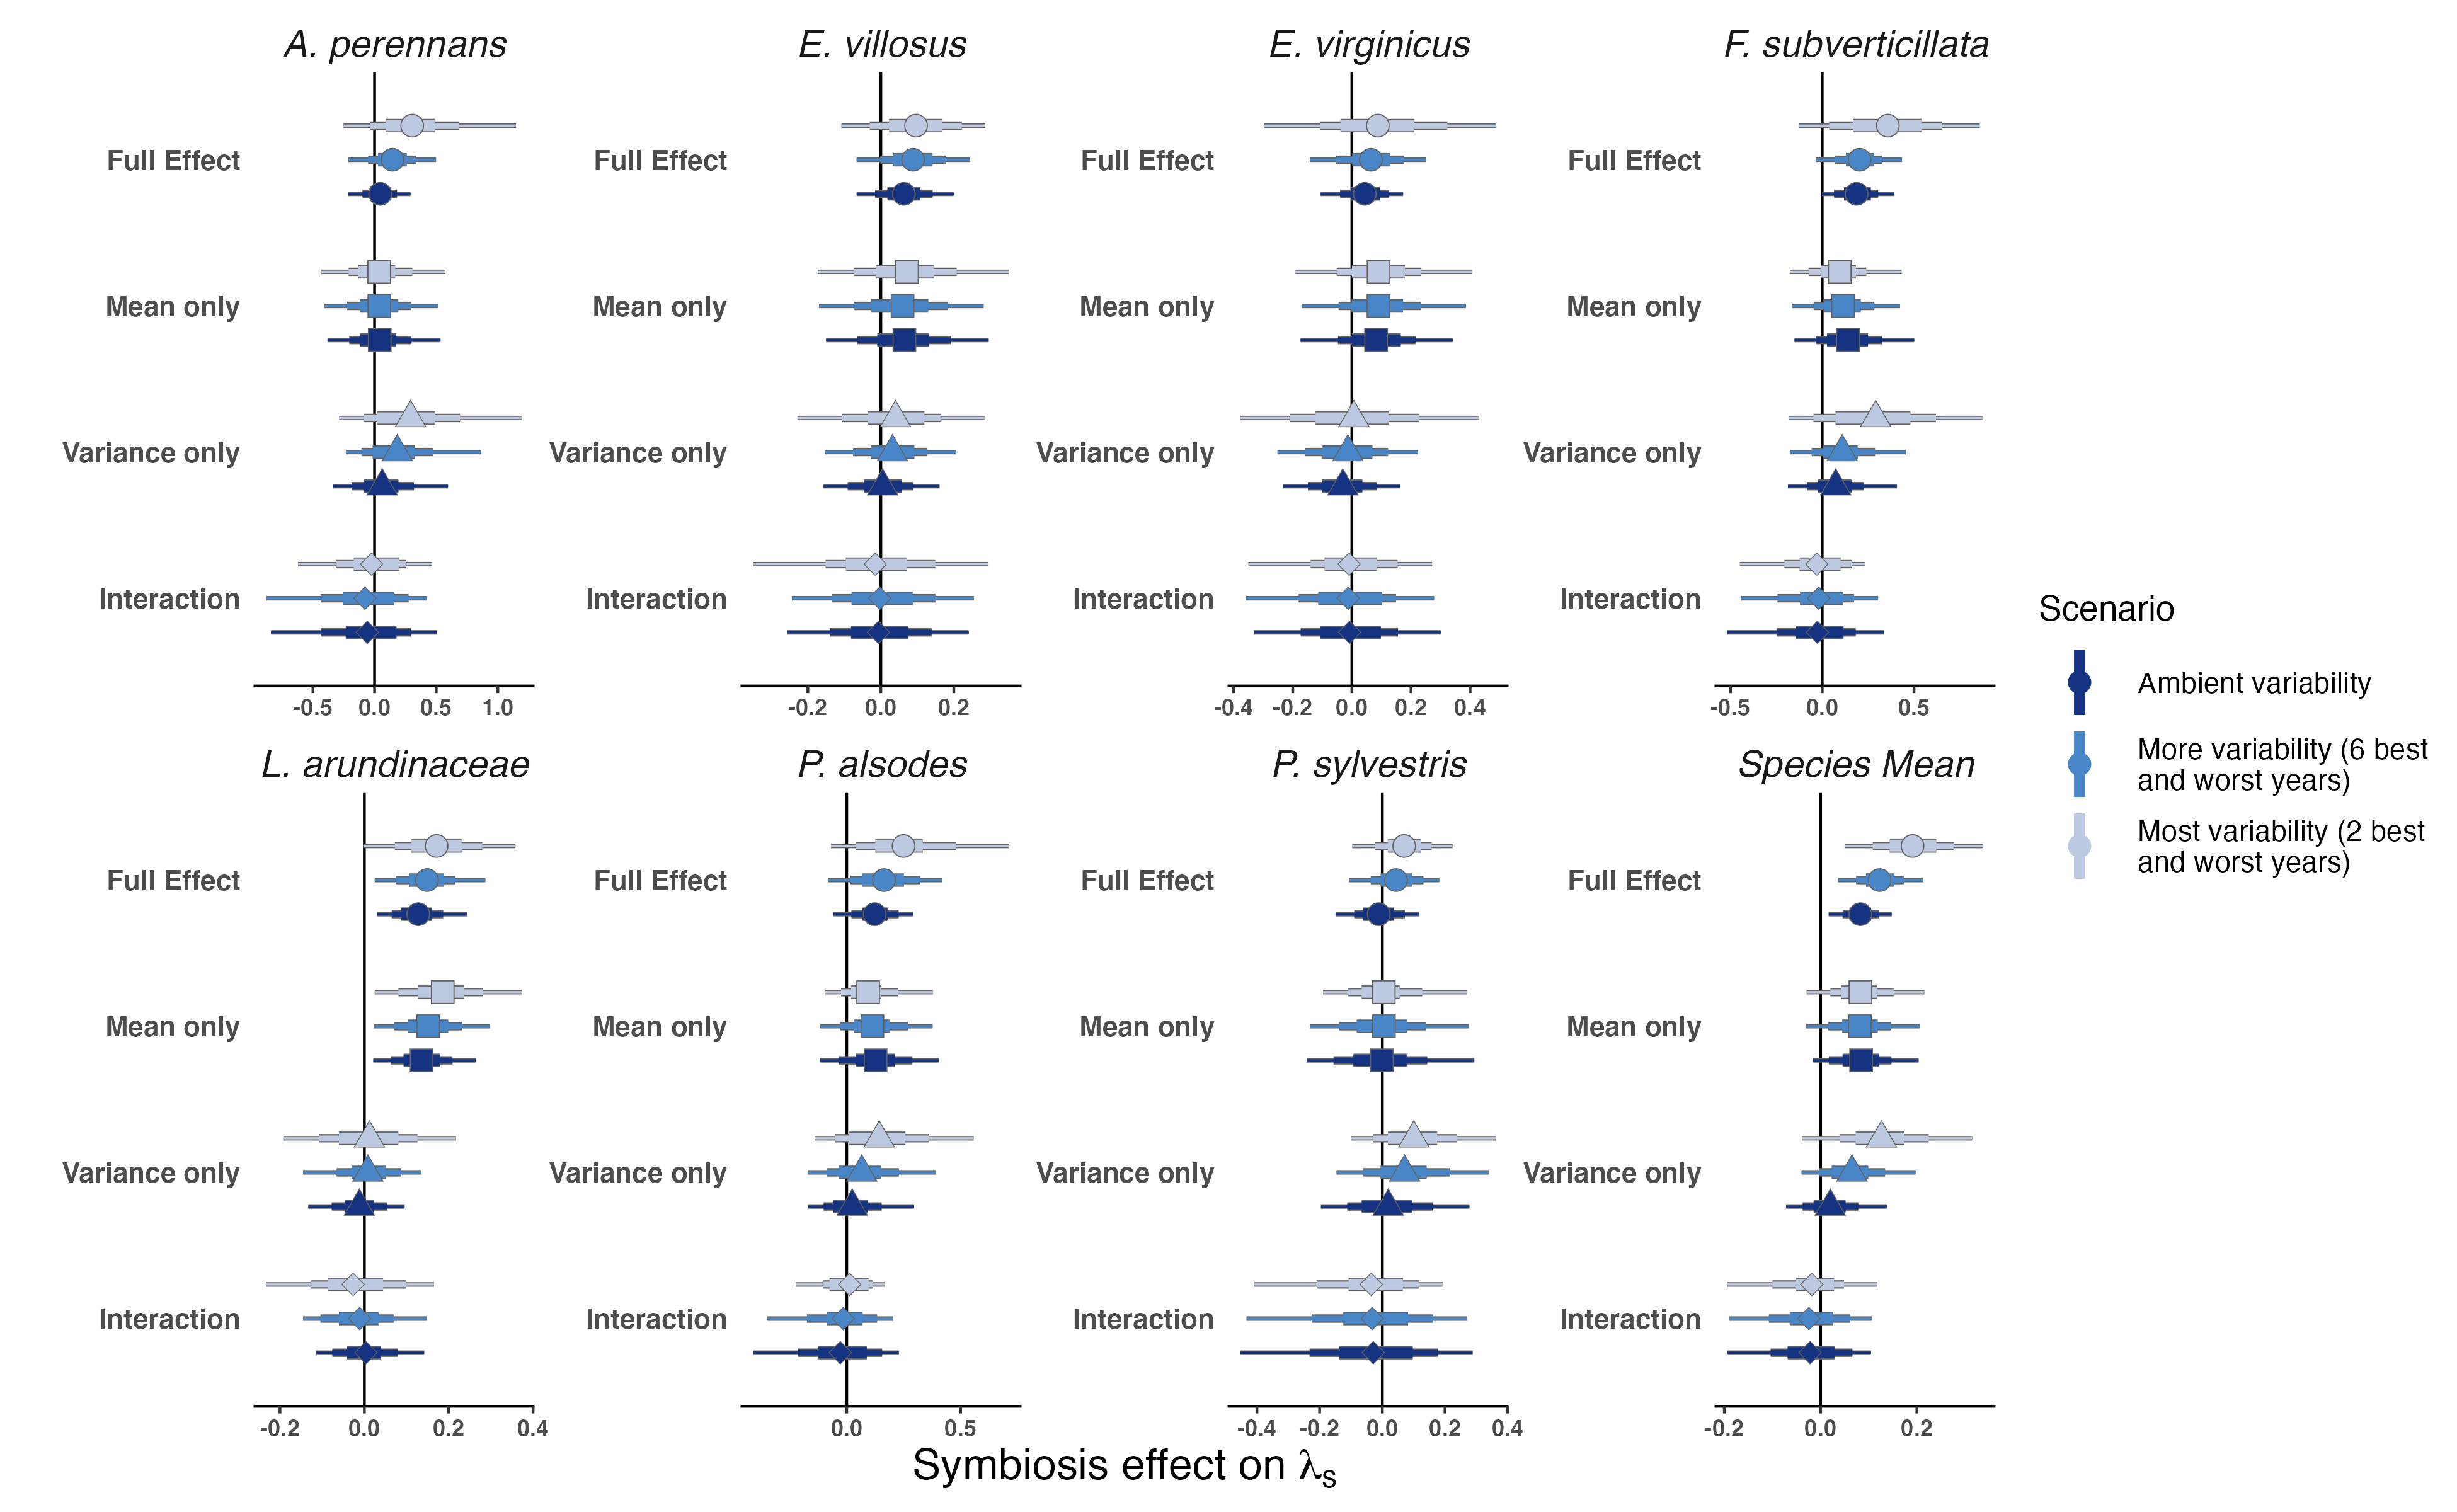
\includegraphics[width=\linewidth]{contributions_obs_plot.png}
	\caption{Endophyte contributions to stochastic growth rates under observed and elevated variance across species. The total effect of endophytes (circle) comes from mean benefits (square) and variance buffering (triangle) as well as the interaction between mean and variance effects (diamond). Shapes indicate the posterior mean of each contribution, along with bars for the 50, 75 and 95 \% credible intervals.  Under scenarios of increasing variance, represented by increasing color intensity, effects of variance buffering increase leading to a more mutualistic symbiosis.}
\end{figure}


\begin{figure}
	\centering
	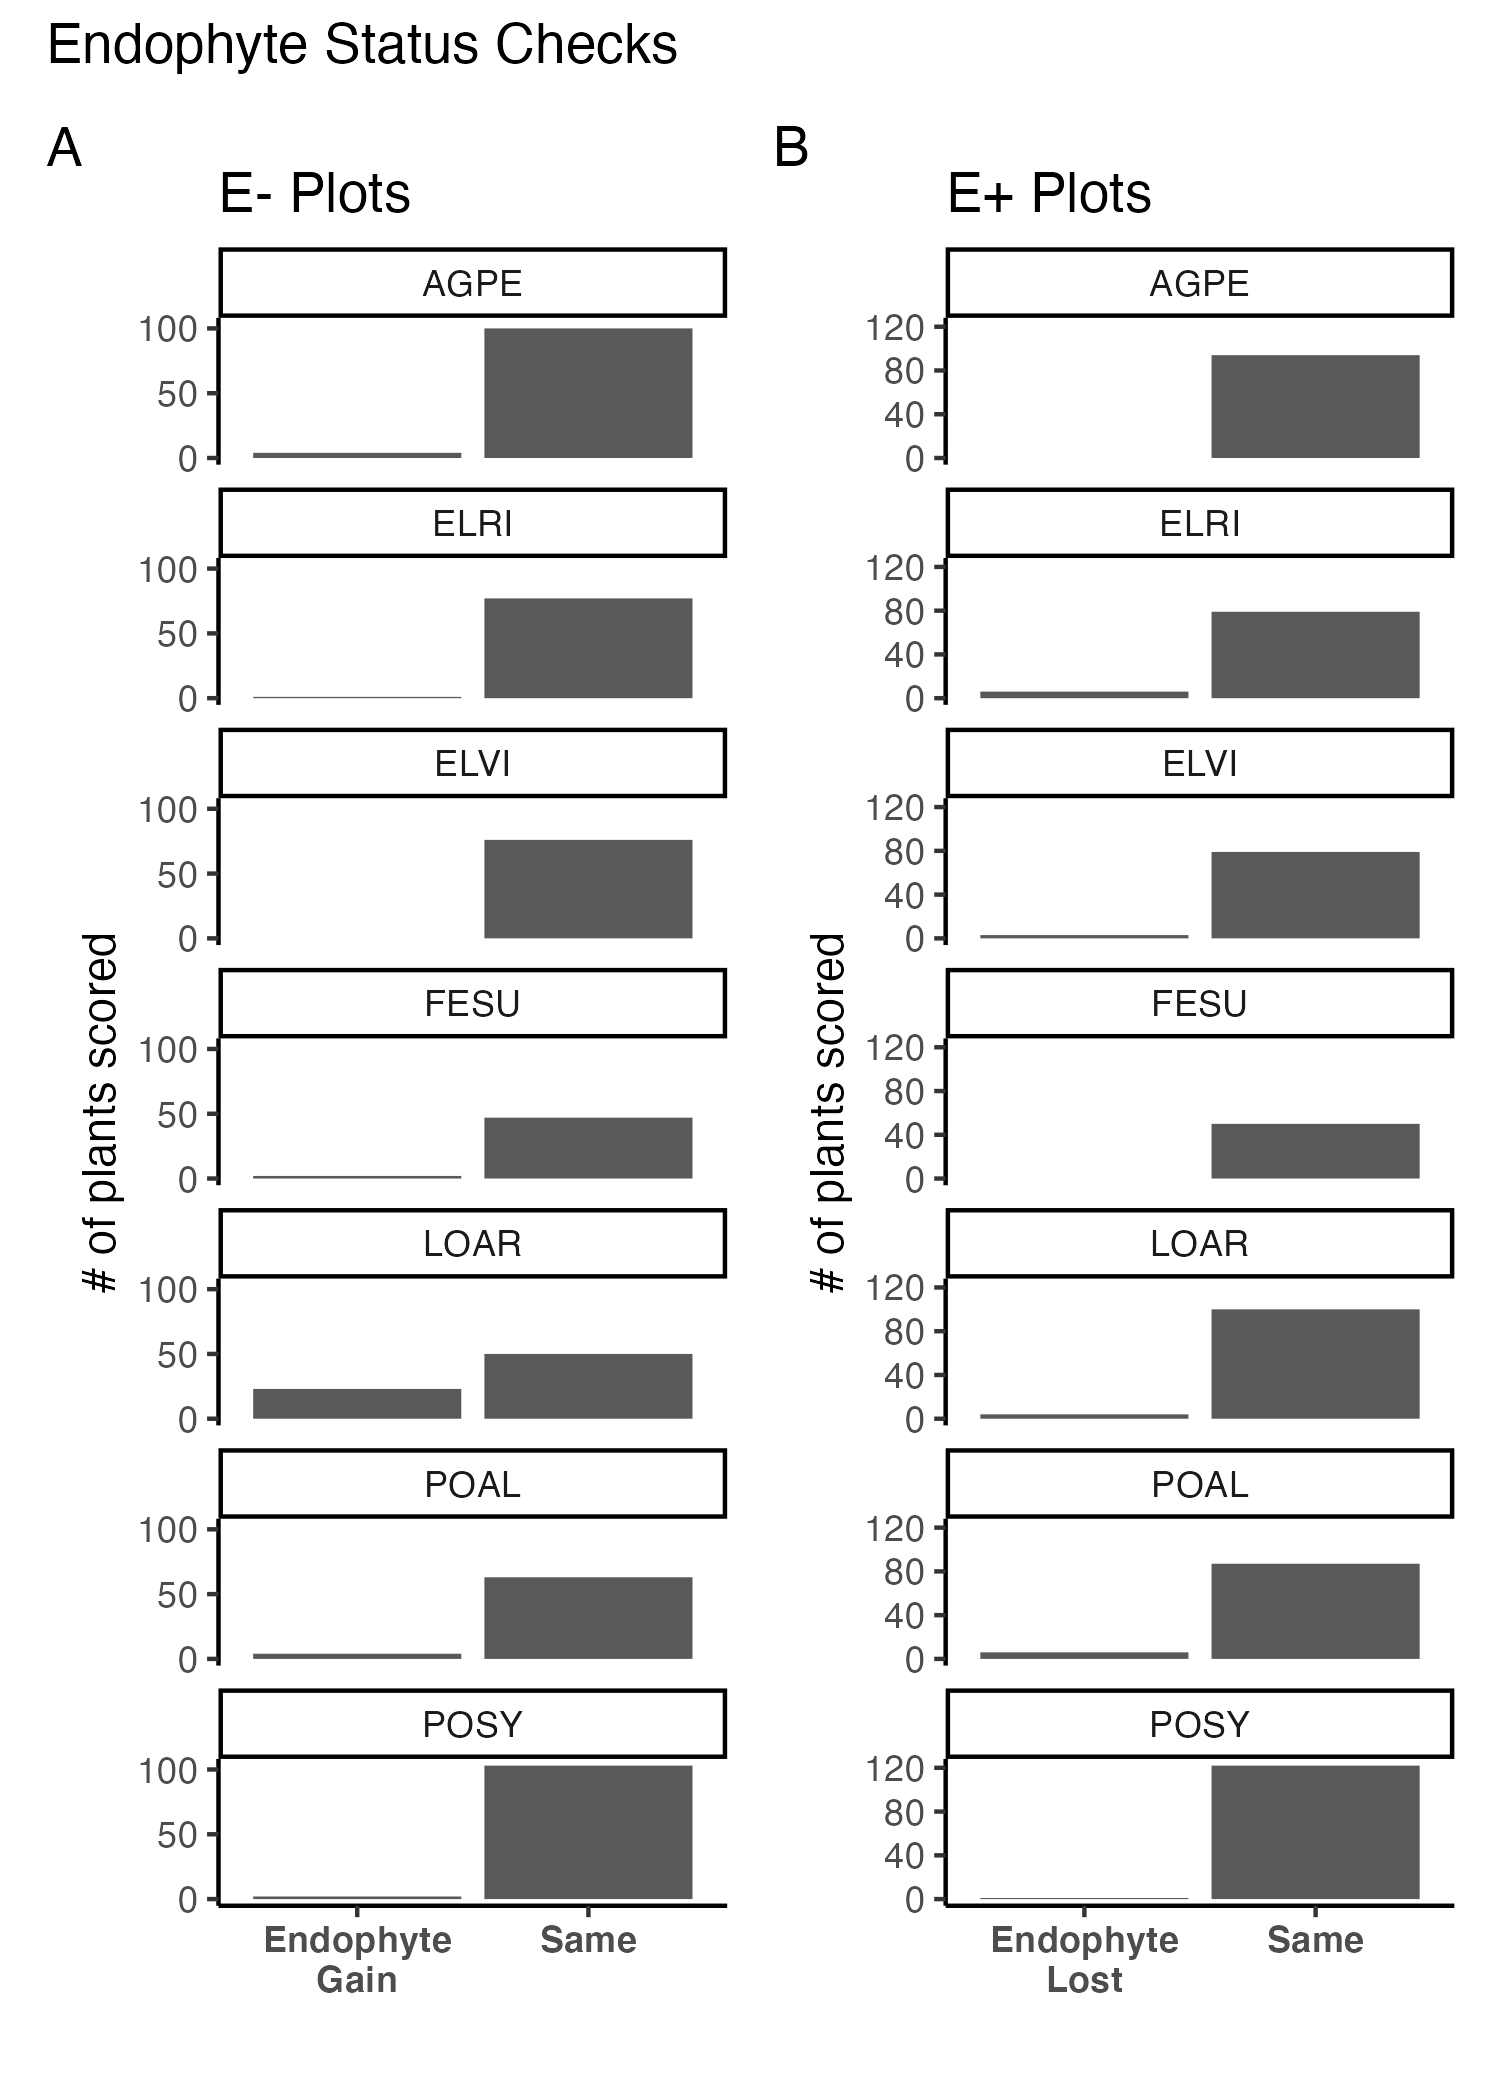
\includegraphics[width=.6\linewidth]{endo_check_plot.png}
	\caption{Faithfulness of experimental plots to assigned endophyte status. Counts of plants scored with leaf peels or seed squashes to check the faithfulness of recruits to the assigned plot-level endophyte status. (A) Endophytic plants may be gained in initially S- plots, or (B) lost in initially S+ plots.}
\end{figure}


\begin{figure}
	\centering
	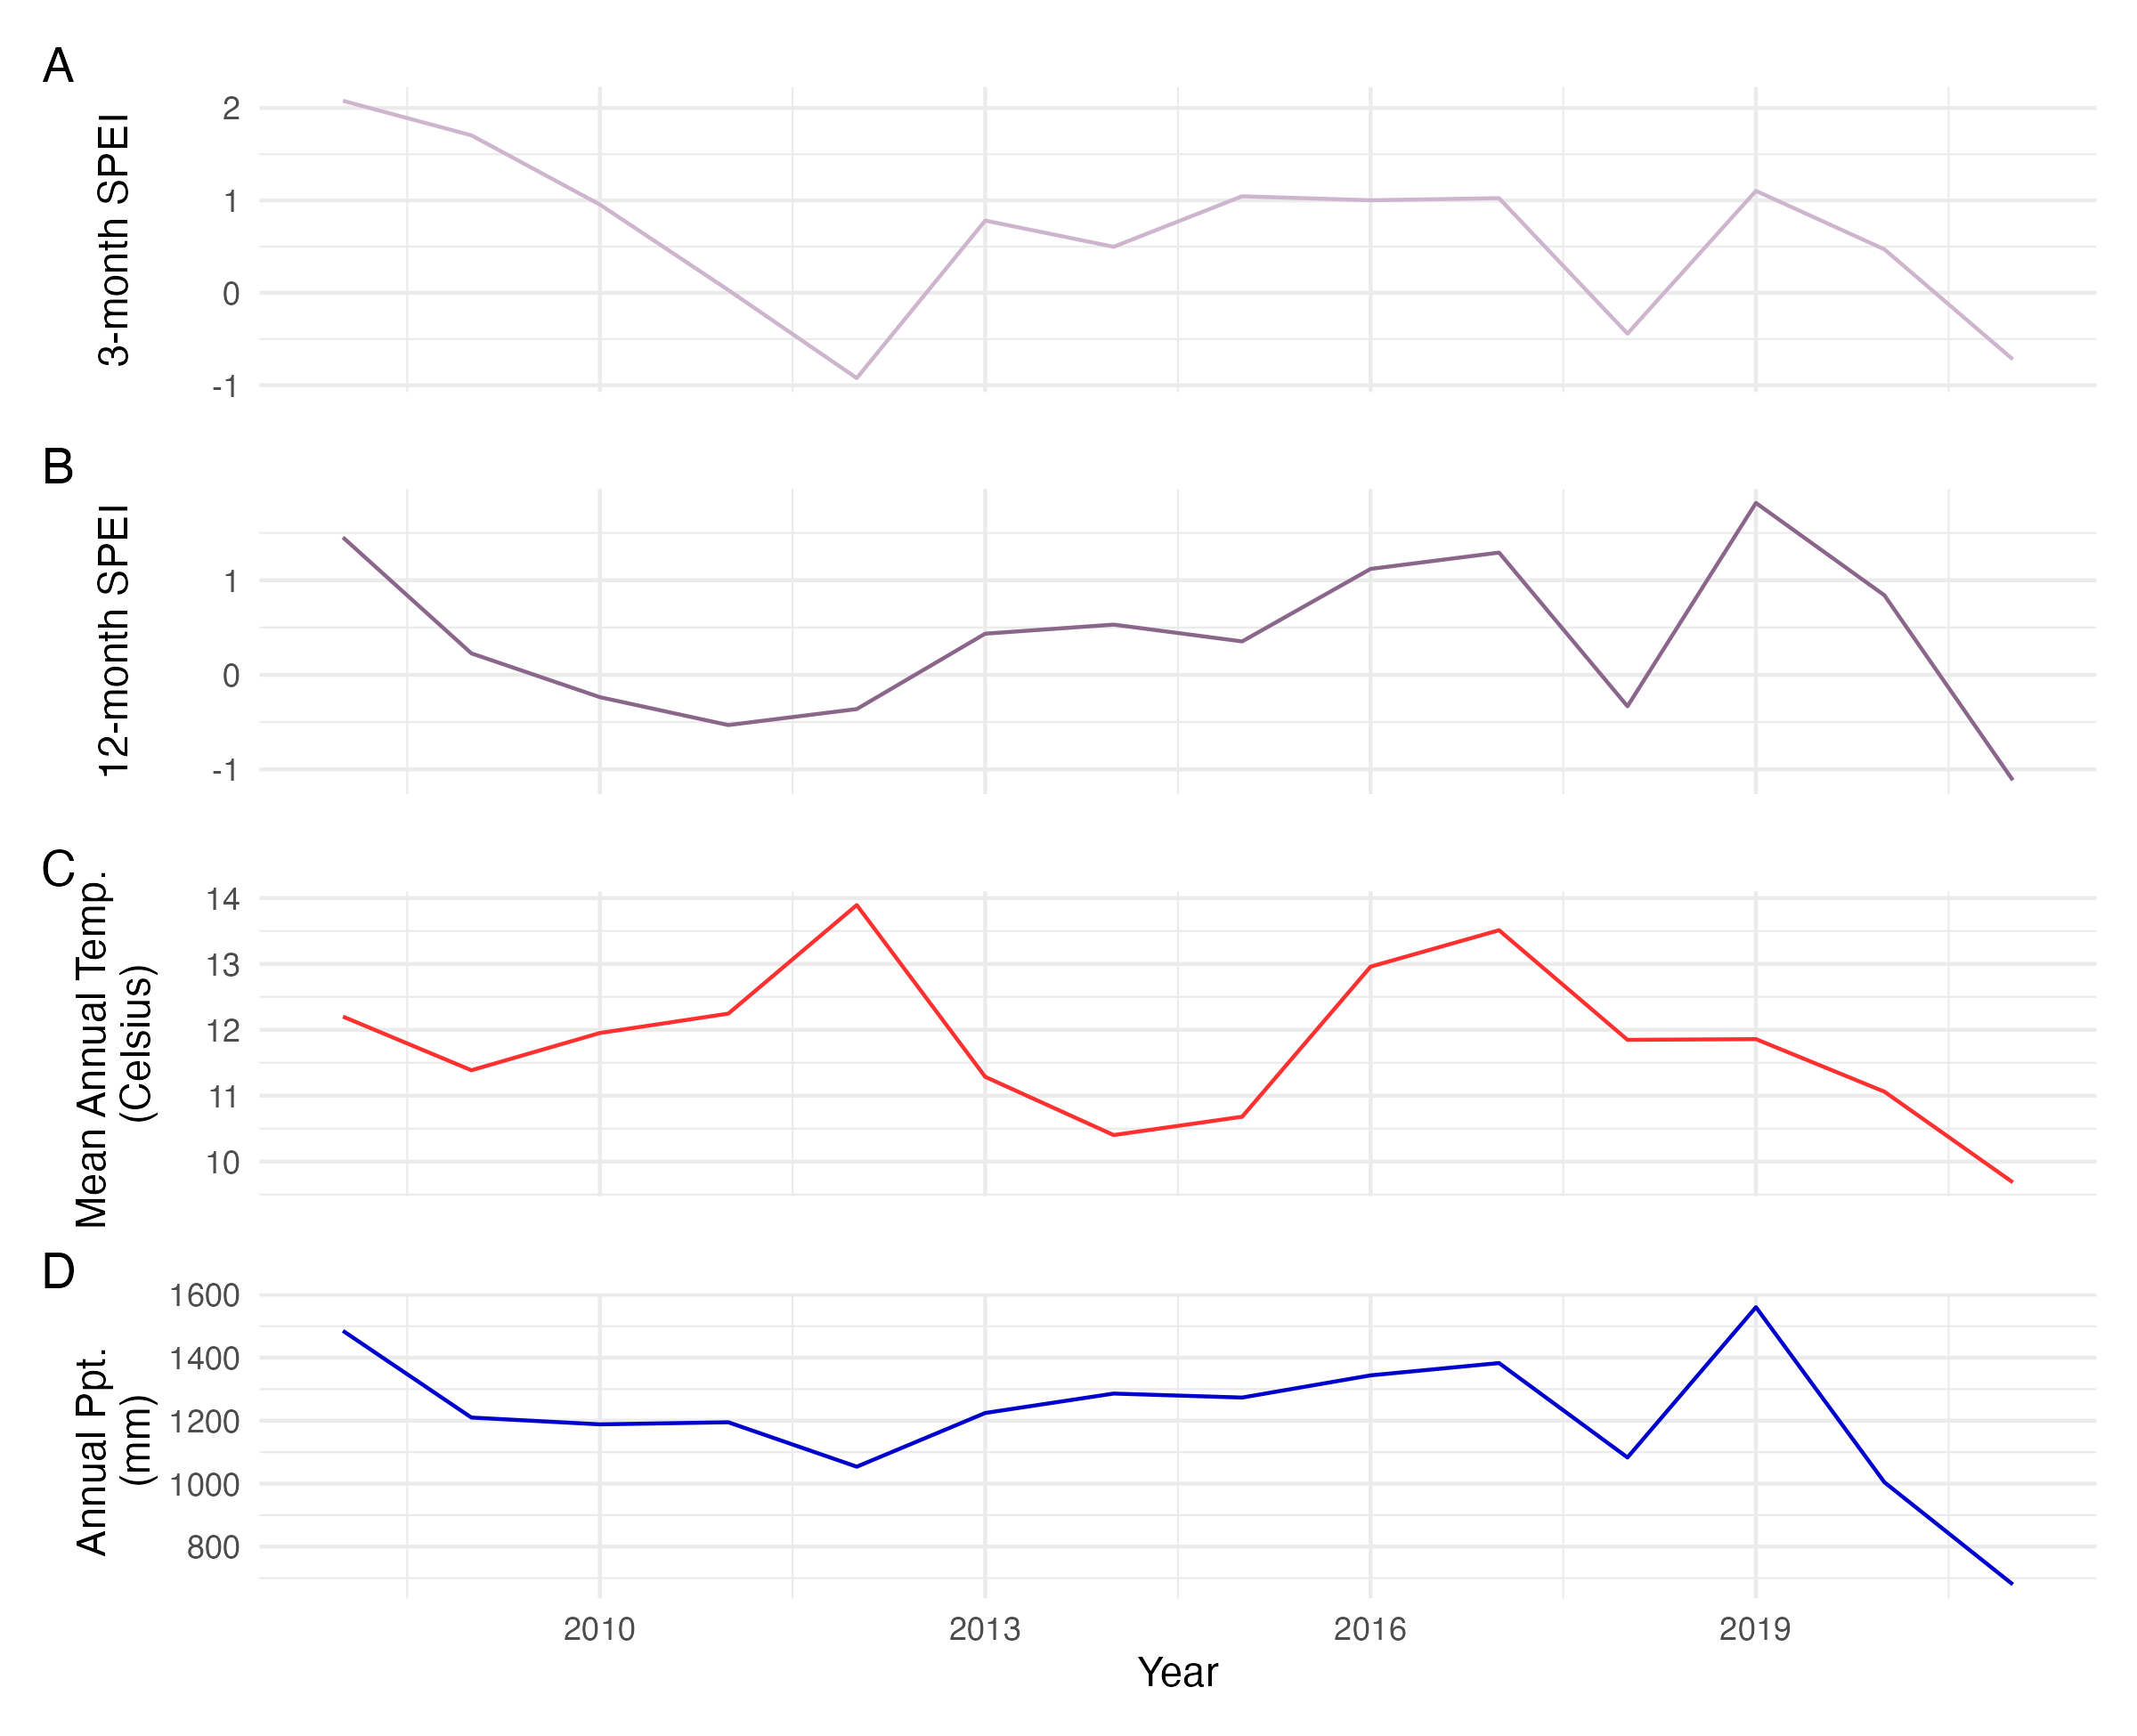
\includegraphics[width=\linewidth]{climate_plot.png}
	\caption{Weather station time-series for Bloomington, IN. The Seasonal Precipitation-Evapotranspiration Index (SPEI) calculated for the (A) three month growing season and (B) annually from daily weather station observations of (C) average temperatures and (D) cumulative precipitation. Climatic data shown are determined by the census year centered on the month of July.}
\end{figure}


\begin{figure}
	\centering
	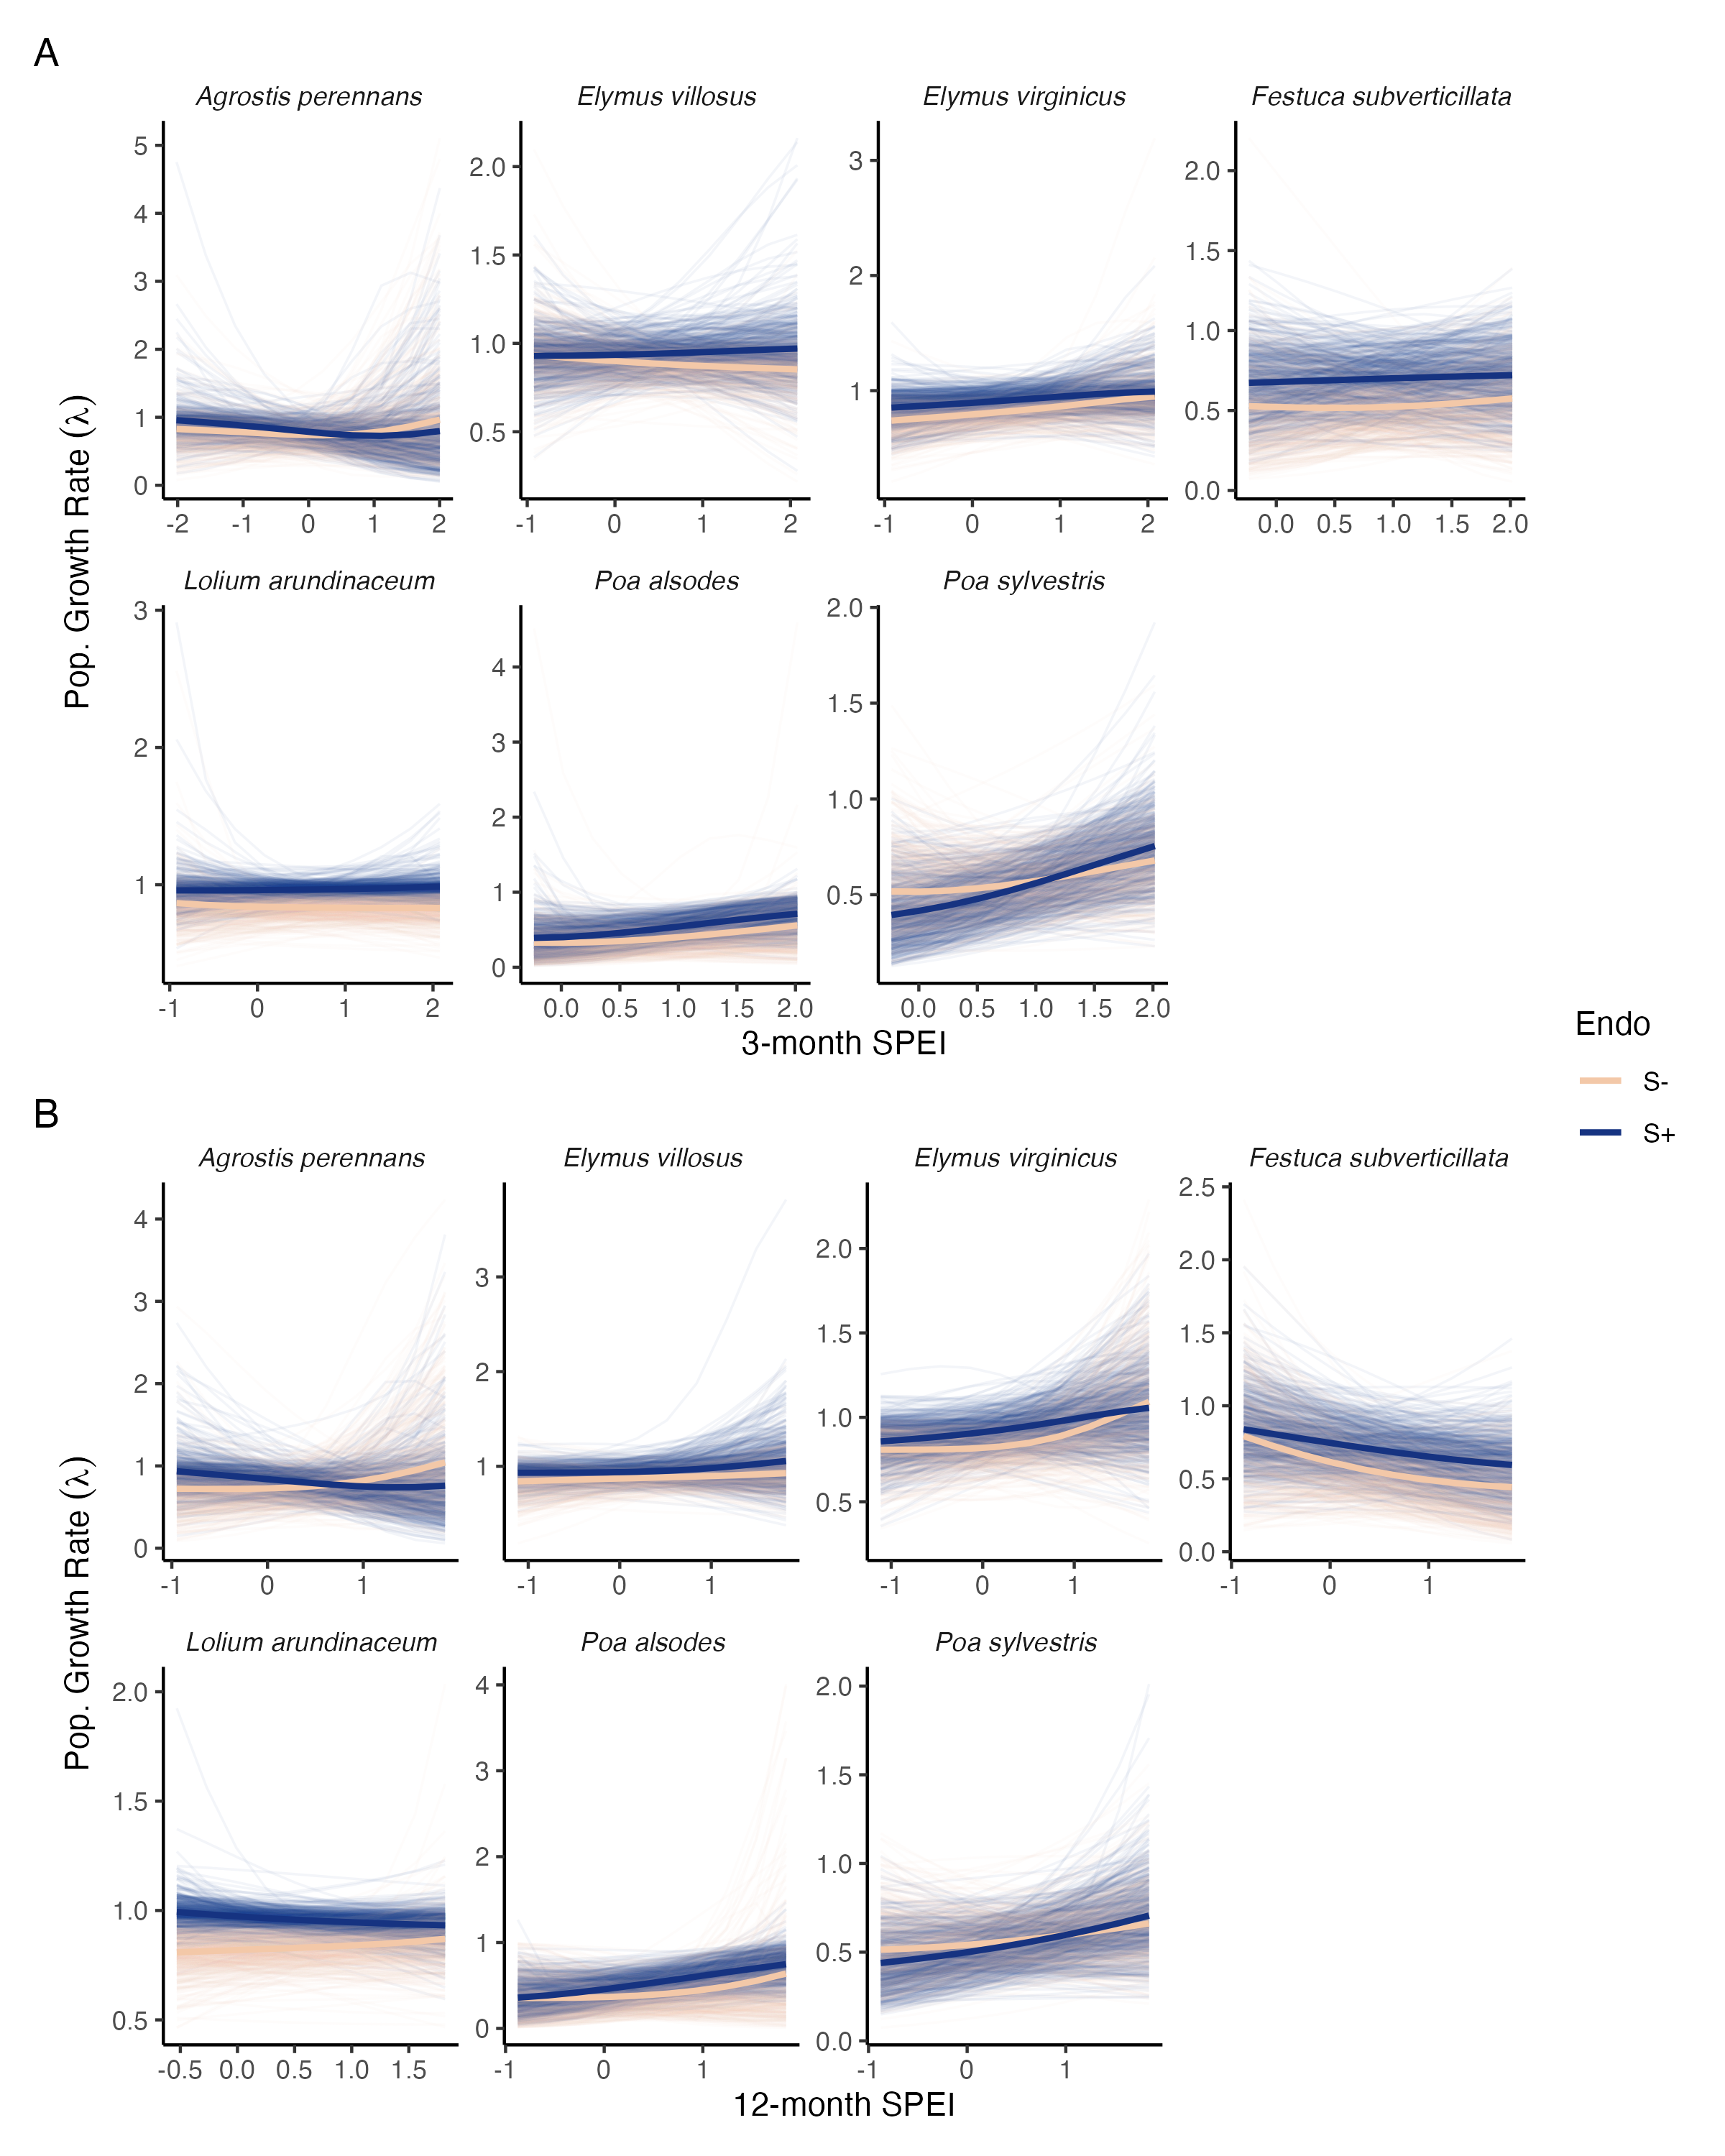
\includegraphics[width=.7\linewidth]{spei_combo_lambda_plot.png}
	\caption{Predicted population growth rates across drought indices. Symbiotic (S+; blue) and symbiont-free (S-; tan) populations respond differently to climate as measured by the (A) 3-month SPEI and (B) 12-month SPEI. Thick lines represent the predicted mean growth rate and thin lines show 500 posterior draws.}
\end{figure}

\begin{figure}
	\centering
	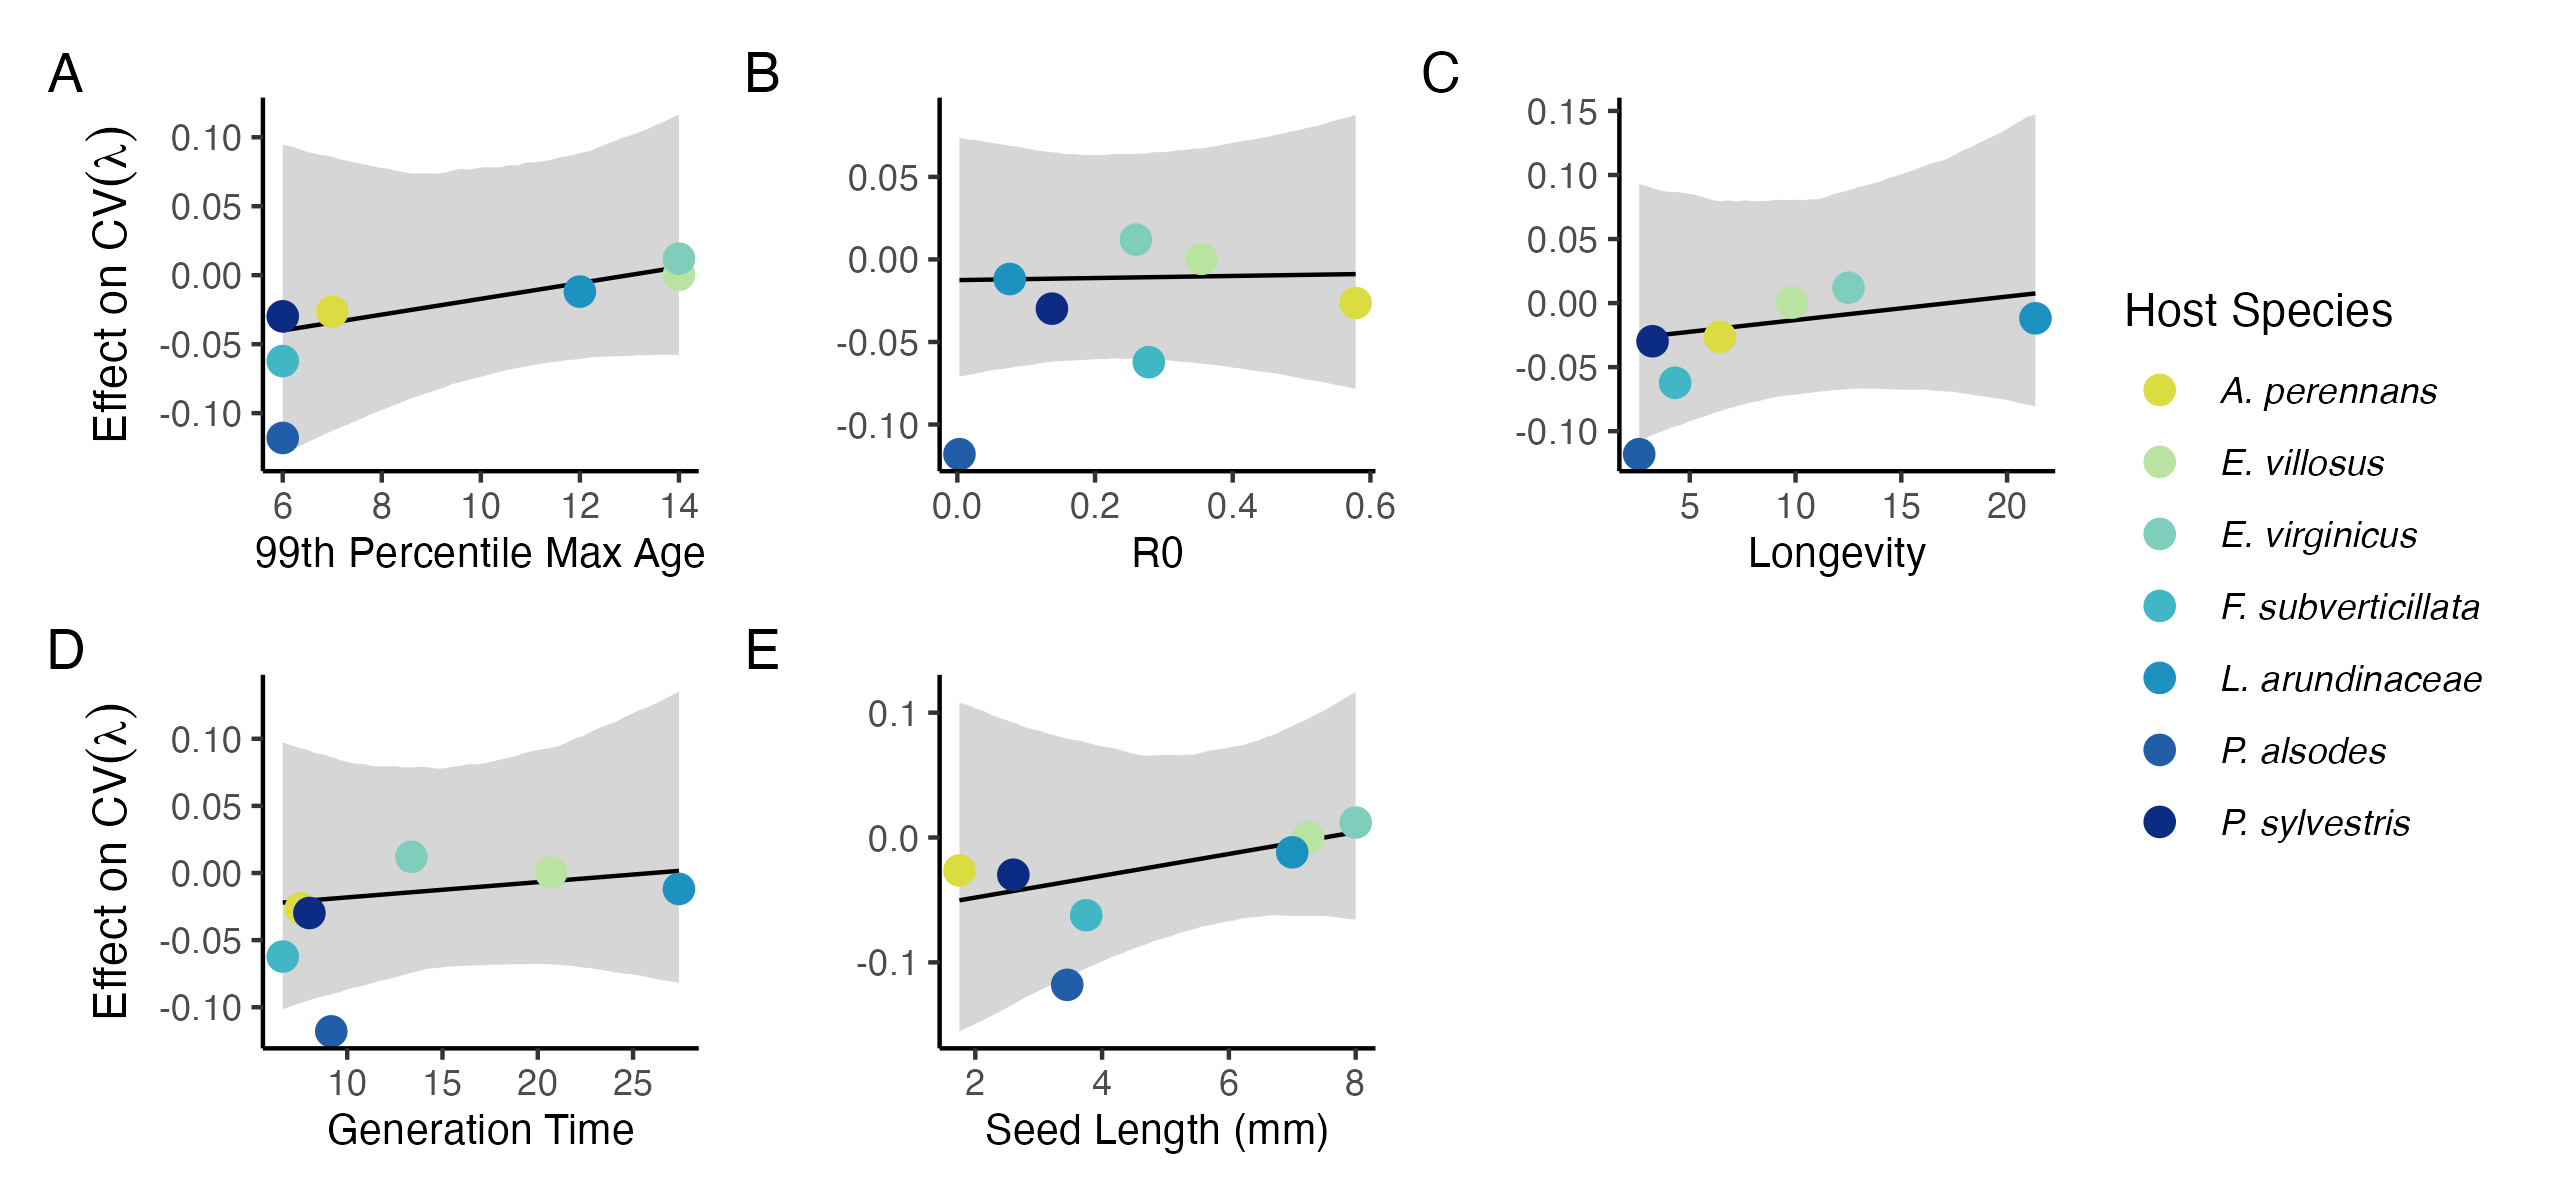
\includegraphics[width=\linewidth]{lh_plant_plot.png}
	\caption{Relationship between variance buffering and life history traits describing the fast-slow life history continuum accounting for phylogenetic covariance between grass host species. Regressions between life history traits describing the fast-slow life history continuum ((A) 99th percentile maximum age observed during long term censuses in years; (B) Net reproductive rate; (C) Longevity; (D) Generation time in years; (G) Seed size) and the effect of endophyte symbiosis on the coefficent of variation in population growth rate ($\lambda$). Each panel shows the fitted mean relationship (line) along with the 95\% credible interval.}
\end{figure}
\newpage

\begin{figure}
	\centering
	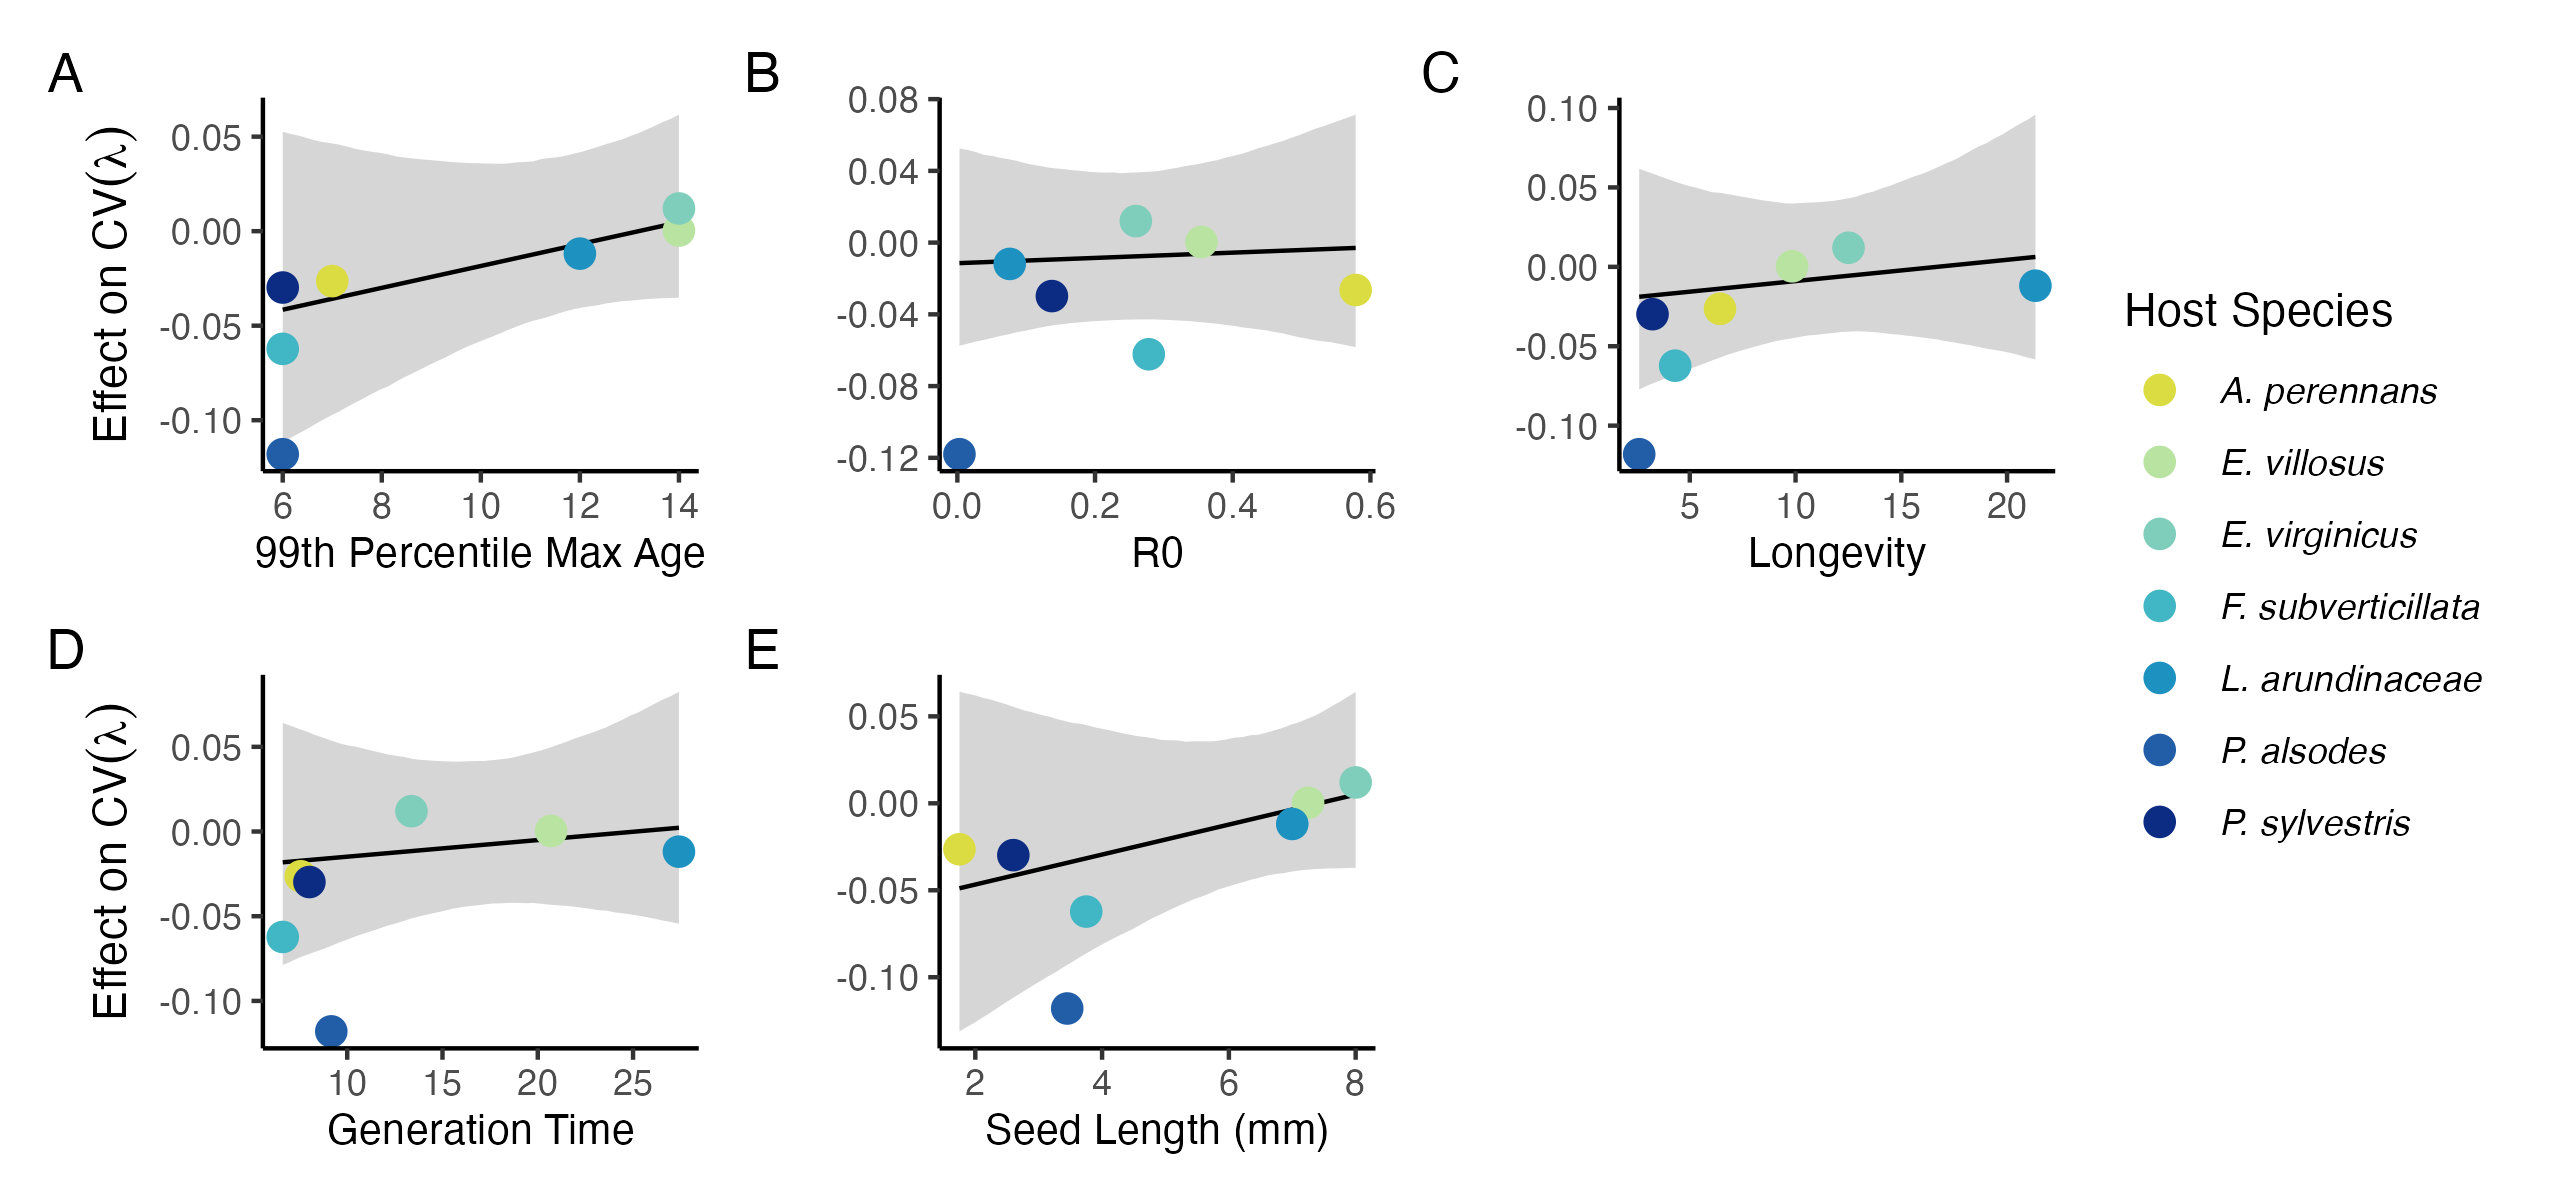
\includegraphics[width=\linewidth]{lh_epichloe_plot.png}
	\label{fig:lh_epich}
	\caption{Relationship between variance buffering and life history traits describing the fast-slow life history continuum accounting for phylogenetic covariance between \emph{Epichlo\"{e}} symbionts. Regressions between life history traits describing the fast-slow life history continuum ((A) 99th percentile maximum age observed during long term censuses in years; (B) Net reproductive rate; (C) Longevity; (D) Generation time in years; (G) Seed size) and the effect of endophyte symbiosis on the coefficent of variation in population growth rate ($\lambda$). Results are similar to regressions accounting for host plant phylogeny (Fig. A25), however symbionts are all within a single genus. Each panel shows the fitted mean relationship (line) along with the 95\% credible interval.}
\end{figure}
\newpage

\begin{figure}
	\centering
	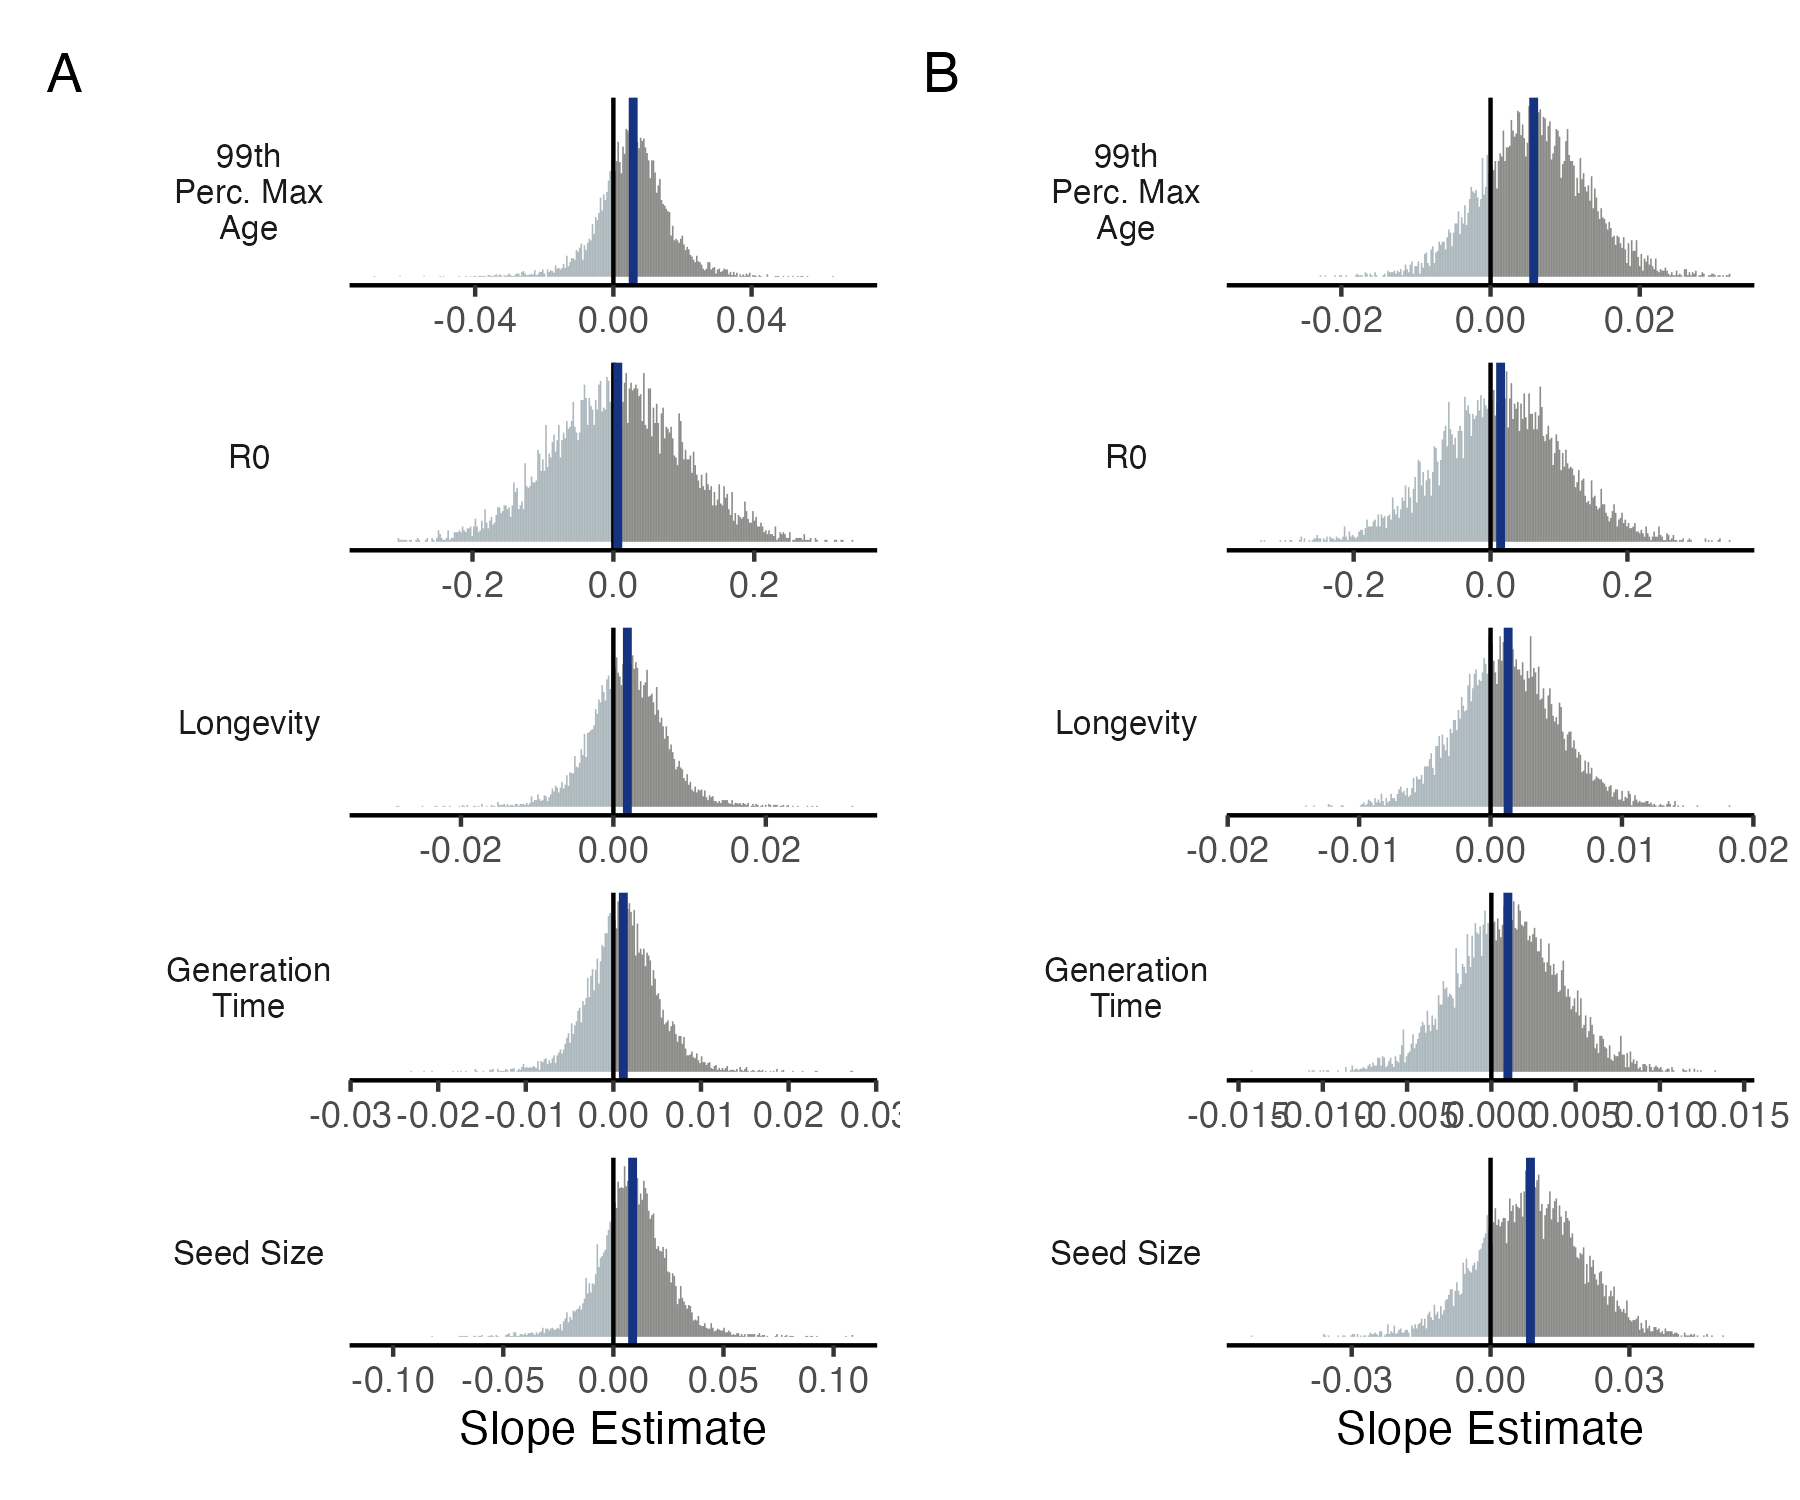
\includegraphics[width=.8\linewidth]{lh_slopes_plot.png}
	\caption{Posterior estimates of life history trait effects on variance buffering. Grey histograms show the posterior distribution of the slope parameter from models incorporating (A) host plant phylogenetic covariance and (B) symbiont phylogenetic covariance for each life history trait with blue bars showing the posterior mean.}
\end{figure}

\clearpage

\subsection*{Supplemental Tables}

\begin{table}\centering
	\caption{Summary of host-endophyte proprogation and transplant methods}
	
	\begin{tabular}{lccc}
			Host Species & Symbiont Species & Heat treatment duration (Temp.)& Transplant date\\
		\midrule
	\emph{Agrostis perennans} & \emph{E. amarillans}&12 min. hot water bath (60 $^{\circ}$C)&April 2008 (10 plots)\\
	\emph{Elymus villosus} &\emph{E. elymi}&6 days drying oven (60 $^{\circ}$C)&April 2008 (10 plots)\\
	\emph{Elymus virginicus} &\emph{E. elymi or EviTG-1}&6 days drying oven (60 $^{\circ}$C)&April 2008 (10 plots)\\
	\emph{Festuca subverticillata} &\emph{E. starrii}&6 days drying oven (60 $^{\circ}$C)&April 2008 (10 plots)\\
	\emph{Lolium arundinaceum} &\emph{E. coenophiala}&6 days drying oven (60 $^{\circ}$C)& Sept. 2007 (10 plots)\\
	\emph{Poa alsodes} &\emph{E. alsodes}& 7 days drying oven (60 $^{\circ}$C)&Sept. 2007 (8 plots)/April 2008 (10 plots)\\
	\emph{Poa sylvestris}&\emph{E. PsyTG-1}&7 days drying oven (60 $^{\circ}$C)& Sept. 2007 (8 plots)/April 2008 (10 plots)\\
		\bottomrule
	\end{tabular}
\end{table}


\begin{table}\centering
		\caption{Summary of focal life history traits }
\begin{tabular}{lp{2cm}p{2cm}p{1.5cm}p{1cm}p{1cm}p{1.5cm}p{1.5cm}p{2cm}}

	Host Species &\raggedright Observed max age (years)& \raggedright 99th percentile max age (years)&Generation time (years) & $\mathbf{R}_0$ &Longevity (years)&Seed Length (mm.)&\raggedright Imperfect transmission rate (\%) & Stromata Observed (\% of indiv. per species)\\
     	\midrule
	\emph{Agrostis perennans} &11&7&7.6&0.58&6.4&1.75&69.8&0.0\\
	\emph{Elymus villosus} &14&14&20.7&0.35&9.8&7.25&100&4.6\\
	\emph{Elymus virginicus} &14&14&13.4&0.25&12.5&8&100&0.6\\
	\emph{Festuca subverticillata} &9&6&6.6&0.28&4.3&3.75&42.7&0.0\\
	\emph{Lolium arundinaceum} &12\footnotemark[1]&12\footnotemark[1]&27.4&0.08&21.3&7&100&0.0\\
	\emph{Poa alsodes} &8&6&9.2&0.003&2.6&3.45&99.9&0.0\\
	\emph{Poa sylvestris}&12&6&8.0&0.14&3.2&2.6&16.6&0.1\\
	\bottomrule

\end{tabular}
\raggedright\footnotesize{*Censuses for \emph{L. arundinaceum} plots stopped after year 12 of the experiment.}
\end{table}

\newpage

\begin{table}\centering
\caption{Summary of host-endophyte drought sensitivities}
\begin{tabular}{lp{1.4cm}p{1.4cm}p{1.5cm}p{1.5cm}p{1.5cm}p{1.5cm}p{1.5cm}p{1.5cm}}
	Host Species& \raggedright Effect on CV($\lambda$)&\raggedright Effect on Mean($\lambda$)&$\frac{\Delta\lambda^{-}}{\Delta SPEI_{3}}$ & $\frac{\Delta\lambda^{+}}{\Delta SPEI_{3}}$ &3 month S- to S+ ratio&$\frac{\Delta\lambda^{-}}{\Delta SPEI_{12}}$ &$\frac{\Delta\lambda^{+}}{\Delta SPEI_{12}}$ & 12 month S- to S+ ratio\\
	\midrule
	\emph{Agrostis perennans} &-0.0264&0.0441&0.03&-0.04&0.85&0.11&-0.06&1.82\\
	\emph{Elymus villosus} &0.0003&0.0509&-0.03&0.01&1.95&0.03&0.04&0.70\\
	\emph{Elymus virginicus} &0.0120&0.0578&0.07&0.05&1.50&0.10&0.07&1.42\\
	\emph{Festuca subverticillata} &-0.0622&0.1639&0.02&0.02&1.01&-0.13&-0.09&1.43\\
	\emph{Lolium arundinaceum} &-0.0118&0.1022&-0.01&0.01&1.32&0.03&-0.03&1.02\\
	\emph{Poa alsodes} &-0.1179&0.1282&0.10&0.14&0.71&0.11&0.14&0.73\\
	\emph{Poa sylvestris}&-0.0298&-0.0085&0.07&0.16&0.44&0.05&0.10&0.55\\
	\bottomrule
\end{tabular}
\end{table}



%%% Add this line AFTER all your figures and tables
\FloatBarrier


\bibliography{endo_stoch_demo}

\end{document}
